%=================================================================
% This template is based on IMRT Latex template by Eric A. Mueller
%================================================================= 

\documentclass[10pt,twoside,a4paper]{report}

 \usepackage[bt,fs,english]{ethasl}   % New styles and commands
                                      % Options: 	bt/mt: Bachelorthesis/Masterthesis
                                      %						fs/hs: Fr�hlingssemester/Herbstsemester
                                      %						german/english: Deutsch/English

% \includeonly{}                      % Quick formatting
% \usepackage[draft]{graphicx}        % Quick formatting

 \usepackage{a4}                      % Paper size
 \usepackage[latin1]{inputenc}        % Keybord settings
 \usepackage{amsmath}                 % Additional math functionality
 \usepackage{amssymb}                 % Additional math functionality
 \usepackage{graphicx}                % EPS figures
 \usepackage[dvips]{epsfig}           % EPS figures
 \usepackage{float}                   % Placement of floating objects
 \usepackage{fancyhdr}                % Headings
 \usepackage{rotating}
 \usepackage{multirow}
 \usepackage{url}
 \usepackage{colortbl}
% \usepackage{ifpdf}% Graphics
 \usepackage{enumerate}				  % Individual enumerate lables [(1)] or [i] [I] [a] [A]
 \usepackage{siunitx}
% \usepackage[thinqspace, amssymb, Gray, textstyle]{SIunits}
% \usepackage{units}					  % Well typesetting of units
 \usepackage{booktabs}					% tables
 \usepackage{tabularx}					% tables
 \usepackage{array}						% vertical alignment in tables

 \newcommand{\ktilde}{$_{\widetilde{}}\,$}
 
% -----------------------------------------------
\usepackage{listings}
\usepackage{color}
\usepackage{textcomp}
\definecolor{listinggray}{gray}{0.9}
\definecolor{lbcolor}{rgb}{0.99,0.99,0.99}
\lstset{
	backgroundcolor=\color{lbcolor},
	tabsize=4,
	rulecolor=,
	language=xml,
        basicstyle=\scriptsize,
        upquote=true,
        aboveskip={1.5\baselineskip},
        columns=fixed,
        showstringspaces=false,
        extendedchars=true,
        breaklines=true,
        prebreak = \raisebox{0ex}[0ex][0ex]{\ensuremath{\hookleftarrow}},
        frame=single,
        showtabs=false,
        showspaces=false,
        showstringspaces=false,
        identifierstyle=\ttfamily,
        keywordstyle=\color[rgb]{0,0,1},
        commentstyle=\color[rgb]{0.133,0.545,0.133},
        stringstyle=\color[rgb]{0.627,0.126,0.941},
}
% -----------------------------------------
 

 \usepackage{color}
 \usepackage{hyperref}
 
 
 \definecolor{black}{rgb}{0,0,0}
 \definecolor{white}{rgb}{1,1,1}

 \definecolor{darkred}{rgb}{0.5,0,0}
 \definecolor{darkgreen}{rgb}{0,0.5,0}
 \definecolor{darkblue}{rgb}{0,0,0.5}

 \hypersetup{colorlinks
	,linkcolor=black
	,filecolor=black
	,urlcolor=black
	,citecolor=black
 }


 \ifpdf
	\usepackage[update]{epstopdf}
 \else
 \fi

 \usepackage{german}                  % German language "o, "a, use.
%\usepackage{ae}                      % German specials
 \usepackage[english]{babel}

%---------------------------------------------------------------------------

 \setlength{\parindent}{0em}                   % Disable parindent
 \rhead[\thepage]{\nouppercase{\rightmark}}    % Special headings
 \lhead[\nouppercase{\leftmark}]{\thepage}     % Special headings
 \cfoot{}                                      % Special headings

%---------------------------------------------------------------------------

 \title{Human-Machine Interface for Operating a Blimb}
 %\subtitle{bla bla bla}

 
 \studentA{Krebs Matthias}
 \studentB{Ledergerber Anton}
% \studentC{Student 3}
 
 

\supervisionA{Konrad Rudin}
\supervisionB{Mora Javier Alonso}
%\supervisionC{XXX Paul Beardsley XXXXX}
 

%===========================================================================
\begin{document}

%---------------------------------------------------------------------------
% Title page

 \maketitle
 \pagestyle{plain}
 \pagenumbering{roman}

%---------------------------------------------------------------------------
% Declaration of Originality

\pagestyle{empty}
% TODO Modify placeholders in declaration.tex
%!TEX root = Bericht.tex
%---------------------------------------------------------------------------
% Declaration of Originality
%
% TODO Add title, student first/last name, supervisor first/last name.

\section*{Declaration of Originality}

\vspace{1cm}

I hereby declare that the written work I have submitted entitled

\vspace{0.5cm}

% TODO Add title
\textbf{Human-Machine Interface for Operating a Blimb}

\vspace{0.5cm}

is original work which I alone have authored and which is written in my own words.\footnote{Co-authored work: The signatures of all authors are required. Each signature attests to the originality of the entire piece of written work in its final form.}

\vspace{1cm}

\textbf{Authors}

\vspace{0.5cm}

\begin{tabular}{ p{5cm} p{5cm} }
% TODO Add student first/last name
  Anton & Ledergerber \\
  Matthias & Krebs \\
\end{tabular}

\vspace{0.5cm}

\textbf{Supervising lecturer}

\vspace{0.5cm}

\begin{tabular}{ p{5cm} p{5cm} }
% TODO Add supervisor first/last name
  Konrad & Rudin \\
  Javier Mora & Alonso \\
\end{tabular}

\vspace{1cm}

With the signature I declare that I have been informed regarding normal academic citation rules and that I have read and understood the information on 'Citation etiquette' (\url{http://www.ethz.ch/students/exams/plagiarism_s_en.pdf}). The citation conventions usual to the discipline in question here have been respected.

\vspace{0.5cm}

The above written work may be tested electronically for plagiarism.

\vspace{2.5cm}

\begin{tabular}{ p{5cm} p{1cm} p{5cm} }
  \cline{1-1} \cline{3-3}
  Place and date & & Signature \\
\end{tabular}

\vspace{2.5cm}

\begin{tabular}{ p{5cm} p{1cm} p{5cm} }
  \cline{1-1} \cline{3-3}
  Place and date & & Signature \\
\end{tabular}

%---------------------------------------------------------------------------



%---------------------------------------------------------------------------
% Preamble

 %!TEX root = Bericht.tex
%---------------------------------------------------------------------------
% Preface

%\chapter*{Vorwort}

%Bla bla \dots

 %\cleardoublepage

%---------------------------------------------------------------------------
% Table of contents

 \setcounter{tocdepth}{2}
 \tableofcontents

 \cleardoublepage

%---------------------------------------------------------------------------
% Abstract

%\chapter*{Zusammenfassung}
% \addcontentsline{toc}{chapter}{Zusammenfassung}

%Bla bla \dots

% \cleardoublepage

\chapter*{Abstract}
 \addcontentsline{toc}{chapter}{Abstract}

This Bachelors thesis was written within project \textsc{Skye}, which is about a high agile spherical blimp called \textsc{Skye} . Main tasks of this novel system will be image capturing and entertainment. The four tetrahedrally arranged motors of the system can be rotated to thrust into any tangential direction to the hull. With the 8 actuation DOF, the 6 state DOF of \textsc{Skye} can be controlled independently. A camera system consisting of a high quality camera as well as two additional low size cameras for 3D reconstructions and live stream is placed on it. \\
To control the unusual freedom of 6DOF, manual control modes as well as automatic control and a combined manual and automatic control mode have been developed. A combination of a tablet PC with a 3DMouse proofed to be suitable to provide intuitive control. A GUI easily allows to switch between control modes, to display the system's status and even to control the system via a touch interface. The touch input screen is underlaid by a map for translations and the video stream for rotations respectively. For automatic control, optimal trajectories for \textsc{Skye} have been designed and compared. Three approaches to track them have been implemented and tested in a simulation environment.

 \cleardoublepage

%---------------------------------------------------------------------------
% Acknowledgements

%\chapter*{Acknowledgements}\label{chap:Acknowledgements}
% \addcontentsline{toc}{chapter}{Acknowledgements}
\chapter*{Acknowledgements}
 \addcontentsline{toc}{chapter}{Acknowledgements}

Without the help of many individuals this thesis would not have been possible. We received the necessary support from all sides throughout the project to realize this HMI. We would like to thank everybody who helped us during its development and therefore also contributed to the successful rollout where \textsc{Skye} flew smoothly with this HMI through the \textsc{ETH} main building.
\\
\\
Special thanks to Prof. Dr. Roland Y. Siegwart, who gave us the opportunity to do this thesis within project \textsc{Skye} at his institute, the \textsc{ASL}.
\\
\\
Also special thanks to Dr. Paul Beardsley, who constantly motivated us and inspired us with great ideas for an intuitive HMI.
\\
\\
We would also like to express our gratitude and thanks to our supervisors, the PhD students Konrad Rudin and Javier Alonso Mora, for the valuable guidance and advice throughout this thesis.
\\
\\
Out of many more individuals, we would like to mention by name Lorenz Meier, Gerhard R{\"o}thlin and Alexander Rudyk. They especially helped us with their programming skills and would always answer all our questions.
\\
\\
Of course this thesis was only possible because of all the whole team \textsc{Skye}. Thank you very much! It was a pleasure to work with you all!
\\
\\
Finally we would like to express our deepest gratitude to our families and beloved ones, Marina and Eliane. They gave us encouragement and showed great patience when it was most required.
\\
\\
\\
\\
\\
We gained a lot of learning experience in this thesis and it was of real pleasure to see \textsc{Skye} finally fly with the HMI developed in this thesis.
\\
\\
\\
\\
Z{\"u}rich, June 2012\\
\\
Matthias Krebs\\
Anton Ledergerber\\





 \cleardoublepage

%---------------------------------------------------------------------------
% Symbols

%\chapter*{Symbolverzeichnis}\label{chap:symbole}
% \addcontentsline{toc}{chapter}{Symbolverzeichnis}
\chapter*{Symbols}\label{chap:symbole}
 \addcontentsline{toc}{chapter}{Symbols}

%\section*{Symbole}
\section*{Symbols}
\begin{tabbing}
 \hspace*{3cm} \= \kill
  ${\bf r}(t)$			\> State vector \\[0.5ex]
  ${\bf p}(u)$			\> 3 dimensional path \\[0.5ex]
  ${\bf \tilde{p}}(t)$	\> 3 dimensianal trajectory \\[0.5ex]
  $u$ 					\> Parameter for path \\[0.5ex]			
  $t$					\> Parameter for trajectory; time \\[0.5ex]	
  $L_p$					\> Geometrical length of path or trajectory	\\[0.5ex]
  $T_p$					\> Time	length of trajectory \\[0.5ex]
  $G^h$					\> Geometrical continuity of a curve \\[0.5ex]
  $C^h$					\> Parametric continuity of a curve \\[0.5ex]
  $n+1$						\> Number of waypoints \\[0.5ex]
  $n_{knots}+1$			\> Number of knots \\[0.5ex]
 \end{tabbing}

%\section*{Indizes}
\section*{Indices}
\begin{tabbing}
 \hspace*{1.6cm}  \= \kill
 $cl$ \> Closest point on path or trajectory \\[0.5ex]
 $lap$ \> Lookahead point on path or trajectory \\[0.5ex]
\end{tabbing}

%\section*{Akronyme und Abk�rzungen}
\section*{Acronyms and Abbreviations}
\begin{tabbing}
 \hspace*{1.6cm}  \= \kill
 ETH \> Eidgen�ssische Technische Hochschule \\[0.5ex]
 ASL \> Autonomous Systems Lab \\[0.5ex]
 HMI \> Human-Machine Interface \\[0.5ex]
 GUI \> Graphical User Interface \\[0.5ex]
 DOF \> Degree of Freedom \\[0.5ex]
 PX4FMU \> \textsc{Pixhawk} Flight Management Unit \\[0.5ex]
 IMU \> Inertial Measurements Unit \\[0.5ex]
 GPS \> Global Positioning System \\[0.5ex]
 usb \\
 rc \\
 AC DC HAC FAC \\
 NED North-East-Down \\
 API \\
\end{tabbing}

 \cleardoublepage

%---------------------------------------------------------------------------


 \pagestyle{headings}                 % Default headings
 \pagestyle{fancy}                   % Special headings
 \pagenumbering{arabic}

%---------------------------------------------------------------------------
% Chapters

 \chapter{Introduction}\label{sec:introduction}
\graphicspath{{graphics/}{graphics/systems/}}

%\section{Motivation}

\section{Context}
\label{sec:context}
%\textit{Write something about project} \textsc{skye}\textit{, focus projects, ETH and/or ASL, DRZ. Motivation..} 

Within the Bachelor's course in mechanical engineering at the ETH Zurich it is offered to join a focus project instead of focus lectures. A focus project is often a novel or experimental design of a prototype\footnote{Some former projects can be found at \url{http://www.asl.ethz.ch/education/bachelor/focus}.} and elaborated over a period of two semesters within a team of mainly students in mechanical engineering, but often in cooperation with students from interdisciplinary courses. The project is settled at the Autonomous Systems Lab (ASL) at ETH Zurich in cooperation with Disney Research Zurich (DRZ). \\
Project \textsc{Skye} then was a focus project started in autumn \num{2011} and will be continued even after the ``official'' end of the project in summer 2012. The \textit{Rollout} event in the historic main building of ETH Zurich was a unique moment when the prototype wafted over the overwhelmed spectators. \\

\begin{figure}[H]
	\centering
    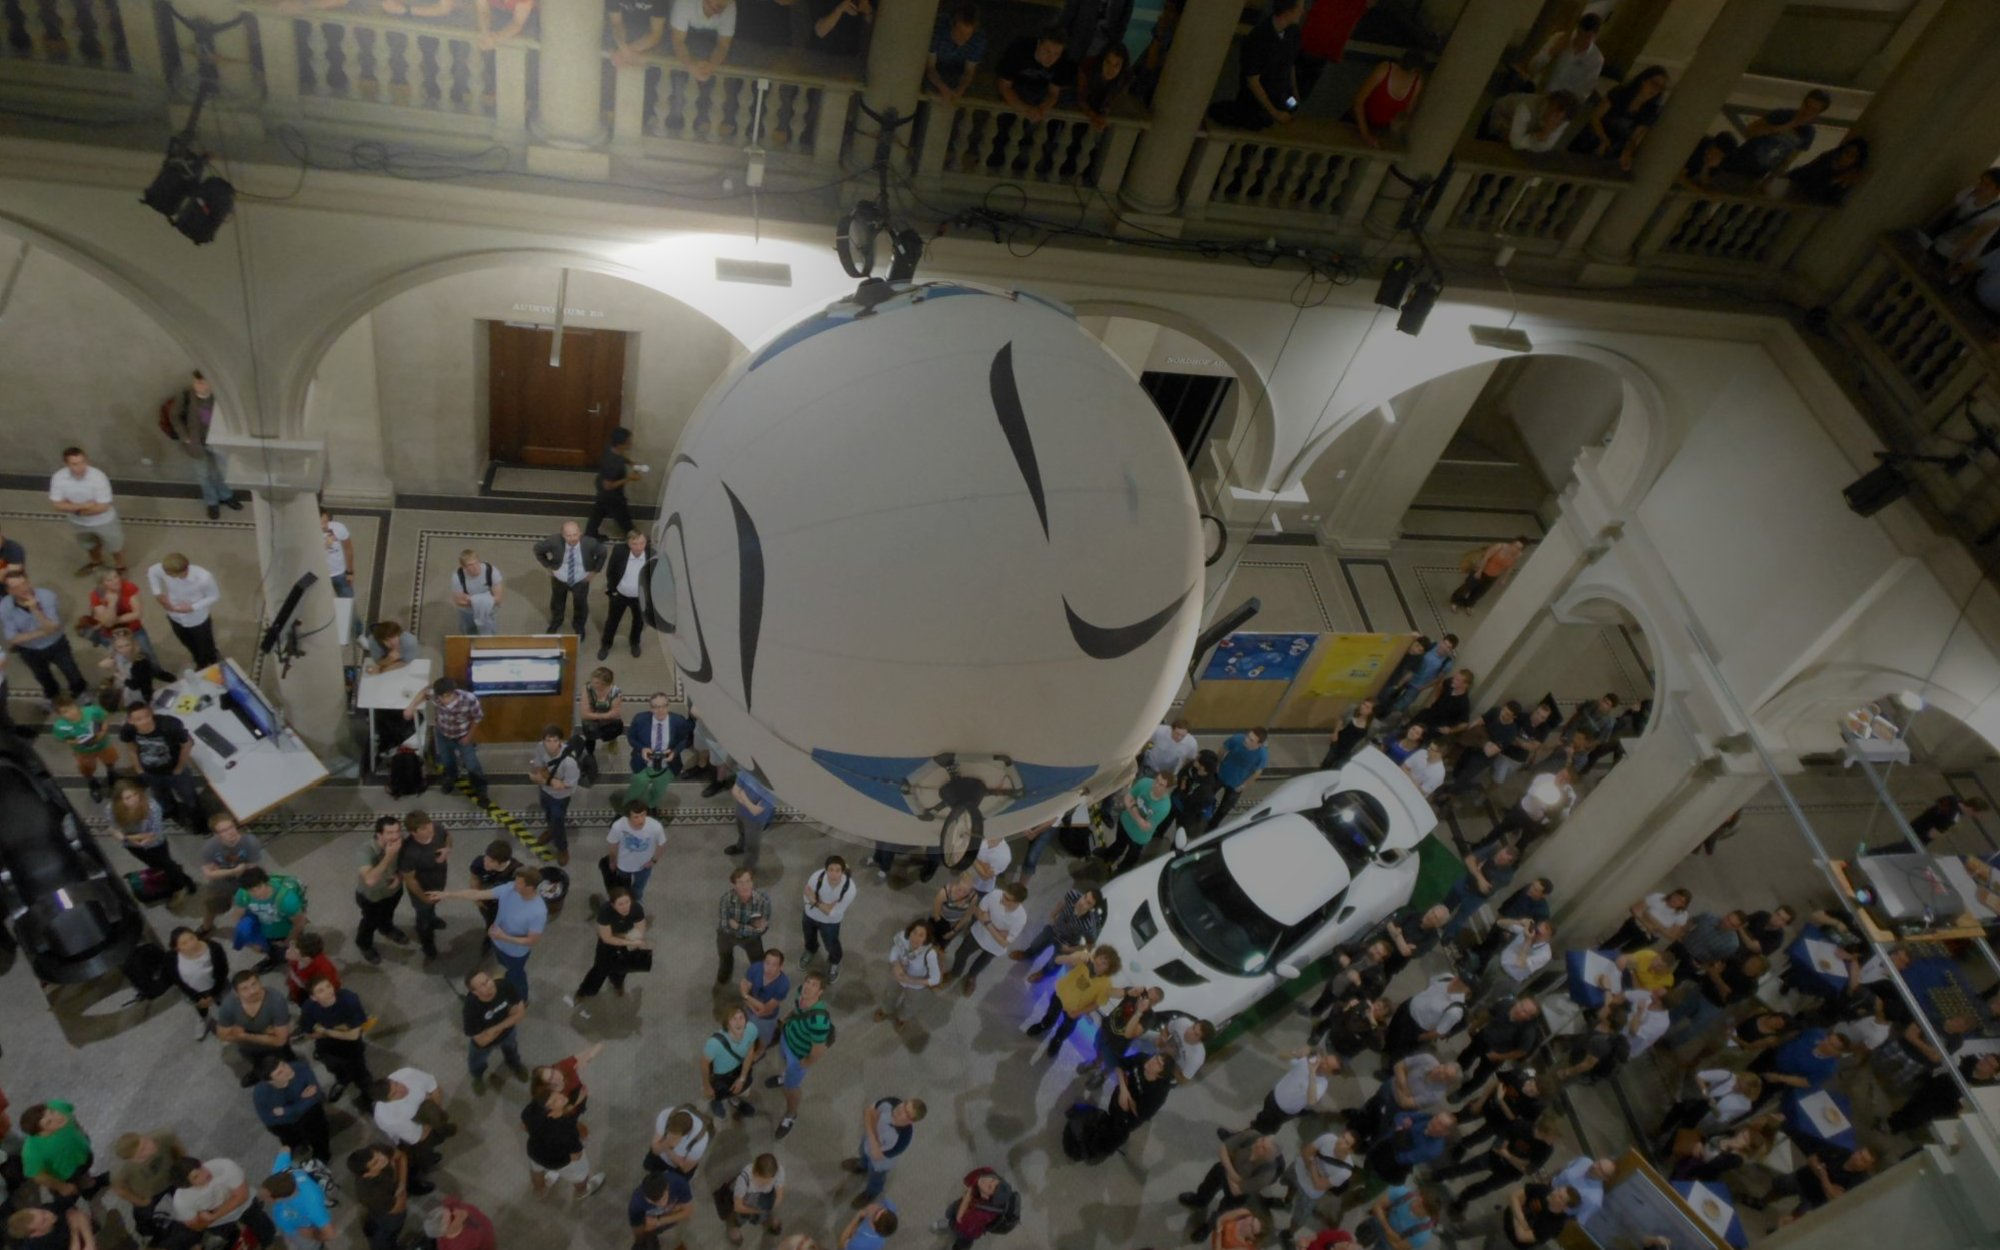
\includegraphics[width = 0.9\textwidth]{graphics/rollout2.jpg}
  \caption{The highligth of project \textit{Skye}: The \textit{Rollout} event on May 25, 2012 in the main hall of ETH Zurich.}
  \label{fig:rollout}
\end{figure}


\section{System Overview}
\label{sec:system overview}
%\textit{Description of \textsc{Skye}. Application fields, technical description, equipment, realization..} \\
\textsc{Skye} is a high agile unmanned aerial vehicle in form of a spherical blimp. It was developed to achieve a system for image capturing for 3D reconstruction as well as obtain entertainment functions (as airshows, human interaction etc.). As there exist already systems that fullfil these requirements\footnote{Mainly quadrotors, but also other UAV.} it was claimed to build a system that provides increased flight time and higher operating safety. \textsc{Skye} is the system that accomplishes these improvements. \\
The two-layered spheric hull is filled with lighter-than-air gas helium. The gas is filled in with an overpressure of \SI{15}{\milli\bar} that ensures a stiff hull surface without the need of any rigid structure. Four identical motor units are placed tetrahedrally on the hull by Velcro. The \textit{AHM 23-10 EPP 1045} thrusters are pointing tangential to the sphere. Their orientation can be rotated around the radial axis using a \textit{\textsc{Maxon} A-Max 16} motor. The center of gravity is approximately identical with the center of buoyancy. Further on, the gravitational force exceeds the buoyancy only for a minimum\footnote{So the system sinks slowly to ground if turned off.}.
\begin{figure}[H]
    \centering
    \def\svgwidth{0.8\columnwidth}
    \input{graphics/skye_description.pdf_tex}
    \caption{CAD sketch of \textsc{Skye}. Red arrows indicate thrust and orientation of the motor units. Blue tetrahedron indicates symmetrical arrangement of them. }
    \label{fig:scene_trajectoryFollowing}
\end{figure}
Further on, a camera system consisting on two light weighted \textit{Bluefox} cameras as well as a high end \textit{Prosilica} high resolution camera connected to a onboard \textit{Intel Atom} embedded computer are detached on the hull. The computer runs a Linux distribution and can be linked to via a Wi-Fi module. A low level \textit{Cortex M4} processor within a \textit{PX4FMU} Inertial Measurement Unit (IMU) controls the flight system. It is equipped with barometer, gyroscope, magnetometer, accelerometer and a GPS receiver. The control communication is realized with both a \textit{Lairtech Xbee} module and a \textit{Futaba Rasst 2.4GHz} receiver. \\
The high symmetrical system properties combined with the 8DOF actuation enable to fully control the holonomic 6DOF space. The 2 additional DOF are used for optimization (see \cite{schaffnervu}).  \\
Finally, the system is only as good as the user appreciates it. Therefore a optimal Human-Machine Interface (HMI) inevitable to provide a useful system. The aim of this thesis is to realize such a HMI in an optimal way for project \textsc{Skye}.
\section{Goals}
\label{sec:goals}
%\textit{Goals of this thesis:
%\begin{itemize}
%\item Define control modes
%\item Develop and realize HMI
%\item Trajectory generating
%\item Trajectory control
%\end{itemize}
%fun.. \\
%}
For this Bachelor's Thesis, intuitive interfaces to control and observe the system \textsc{Skye} had to be developed. This includes the implementation of a Graphical User Interface (GUI) for a computer based Ground Station (GS) based on any existing solution. Further on, different manual control modes and suitable Human-Machine Interfaces must have been elaborated and implemented. Finally, automatic manoeuvres  (paths and trajectories) had to be generated considering simplified dynamic system constraints based on the results from a model elaborated in \cite{weichart}. These goals are summarized in table \ref{tab:goals}. \\
\textbf{
Further on, the successful completion of project \textsc{Skye} could only be realized by invest a lot of effort for the compatibility of all system's part. Especially the integration of an alpha version IMU required thousands of tests to reach a full working system. bla bla Version Control, bla bla, das Zeugs gehoert wohl eher in die Conclusion..} So move it there;-)


\begin{table}[H]
\begin{center}
 \begin{tabular}{ll}
 \hline
 Goal & Specification  \\ \hline \hline
 Control Modes 	& 	Intuitive Control for Manual for 6DOF Blimp \\
 HMI			&	Suitable for Control Modes \\
 GUI         	& 	Provide System Info, Adapt Properties \\
 Trajectories   & 	Automatic Maneuvers \\
 \hline
 \end{tabular}
 \caption{Main goals of this thesis}\vspace{1ex}
 \label{tab:goals}
\end{center}
\end{table}


\section{Similar Systems and their HMI}
\label{sec:similar systems}
%\textit{About degrees of freedom, (non-)holonomic system control, car wheels, rezeros qgo sphere cite \cite{kammermann}.} \\
The HMI (or control device) for a machine mainly depends on its number of control inputs and its level of automation. To control more control inputs, additional sticks or motions have to be provided. Automation of the system can simplify its control, but requests for emergency backups in case of automation fail. \\
The number of control inputs depends on the systems possibilities. This is shown in table \ref{tab:systems_hmi}\footnote{\textsc{AMZ} racing: \url{http://www.amz.ethz.ch/} \\ \textsc{Rezero}: \url{http://rezero.ethz.ch/} \\ \textsc{Arac}: \url{http://www.arac.ethz.ch/} \\ \textsc{arDrone}: \url{http://ardrone2.parrot.com/}}. A car has 3DOF, i.e. it can move in a plane and turn around its yaw axis. But the driver cannot steer all those motions independently as no lateral motion is possible without longitudinal movements (the system has a nonholonomic constraint). So a steering wheel in combination with a gas and break pedal serve as HMI. For a ballbot or a legged robot each of the 3DOF can be steered directly (they are holonomic systems). Therefore the HMI device must enable three inputs as it is provided for instance by a Qgo Sphere\footnote{See \cite{kammermann}, section \ref{sub:hardware} or \url{http://www.quasmo.ch/index.php/qgosphere} for more informations about Qgo Sphere.} or a game-pad. A quadrotor is comparable to the system \textsc{Skye}. A quadrotor is a nonholonomic system, as roll and pitch angle are coupled with the lateral and longitudinal motion. Therefore out of the 6DOF in space, only 4 can be controlled independently by the pilot. A game-pad or even a smartphone are suitable control devices. As \textsc{Skye} is (due to its mechanics and actuation symmetry) a holonomic system, all the 6DOF can be steered individually. This requires a HMI with even more control inputs.
%In a car, the driver controls the steer angle and the acceleration. Although this is not sufficient to move the car into any desired direction\footnote{As the lateral motion depends on the turning angle, the system is nonholonomic.} the steering wheel and gas pedal provide sufficient and intuitive control to drive from a to b. The pilot of an airplane can move through the three dimensional space and has therefore more freedom to control its vehicle than the car driver. As a drawback, he has to consider even more control inputs (joystick for pitch and roll, rudder pedals for yaw and throttle control for thrust). As the system dynamics of \textsc{Skye} only depend on holonomic constraints, its motion in the 3D space can be controlled for every of the 6DOF independently. As a drawback, the pilot would have to consider 6 control inputs at the same time. The elaboration of finding a suitable solution for the piloting of \textsc{Skye} is described in chapters \ref{cha:DifferentControlModes} and \ref{cha:findHardSoftSolution}.

\begin{table}[H]
\begin{center}
\newcolumntype{M}{>{$\vcenter\bgroup\hbox\bgroup}c<{\egroup\egroup$}} 
 \begin{tabular}{MMMMM}
 \hline
 System & DOF & Non\-holonomic & Inputs & Device \\ 
  \hline \hline 
     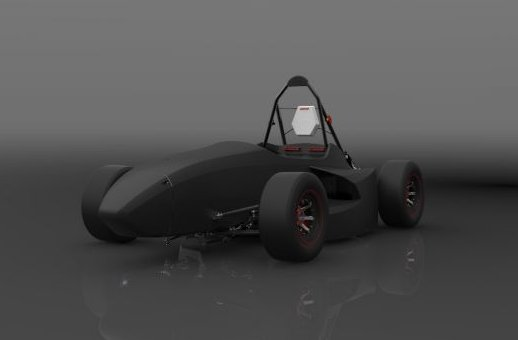
\includegraphics[width = 0.25\textwidth]{amz.jpg}
   & 	3 & 1  & 2 & 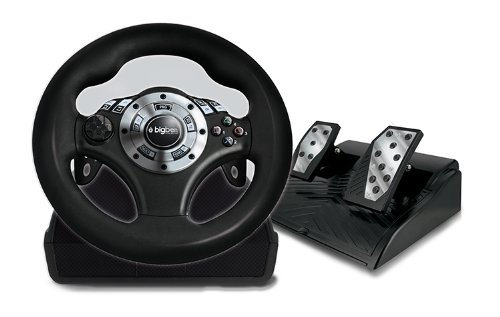
\includegraphics[width = 0.18\textwidth]{steeringwheel.jpg} \\
  \hline
    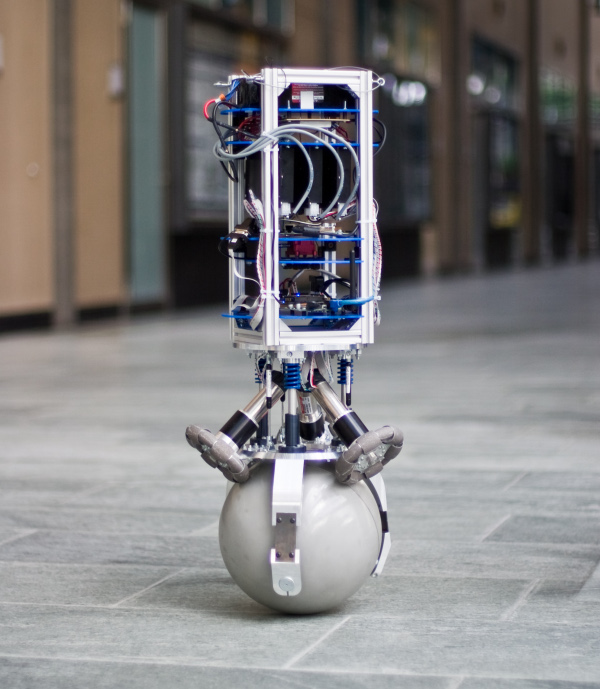
\includegraphics[width = 0.25\textwidth]{rezero.jpg}
   & 	3 & 0  & 3 & 
\includegraphics[width = 0.18\textwidth]{HMI/qgo_sphere_cut.jpg} \\
  \hline
    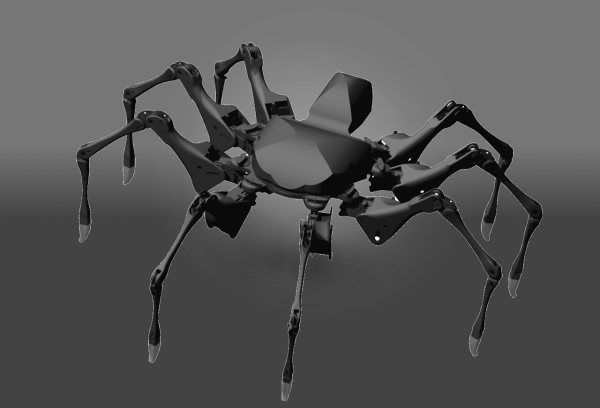
\includegraphics[width = 0.25\textwidth]{arac.jpg}
   & 	3 & 0  & 3 & 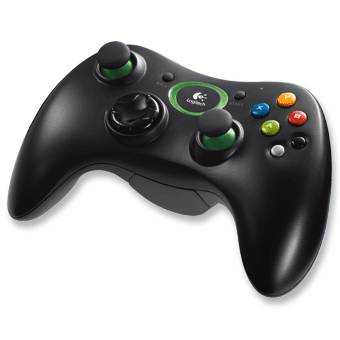
\includegraphics[width = 0.14\textwidth]{gamepad.jpg} \\
  \hline
    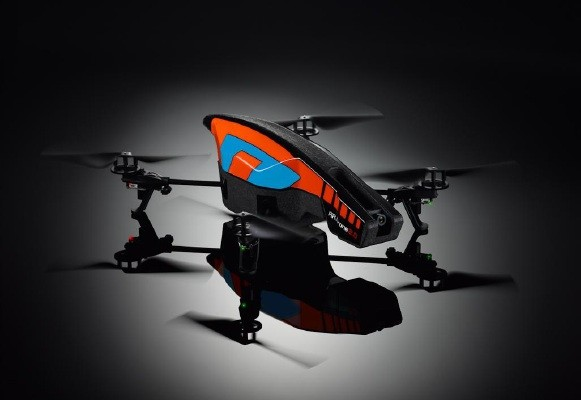
\includegraphics[width = 0.25\textwidth]{ardrone.jpg}
   & 	6 & 2  & 4 & 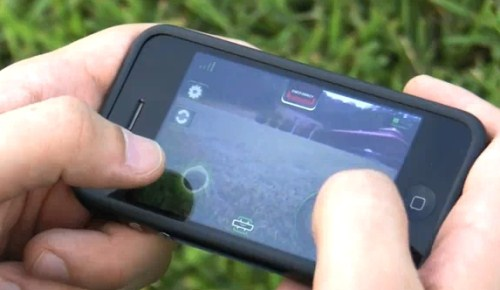
\includegraphics[width = 0.18\textwidth]{iphone.jpg} \\
  \hline
    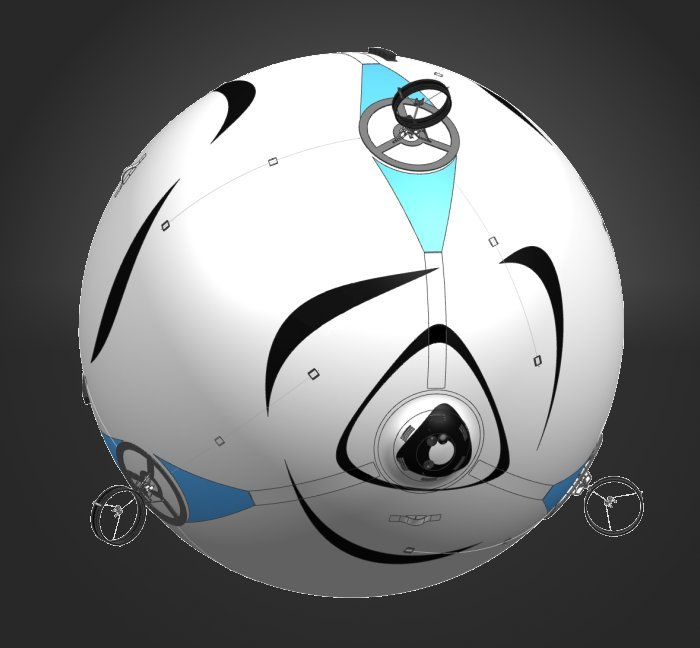
\includegraphics[width = 0.25\textwidth]{skye.jpg}
   & 	6 & 0  & 6 & 
\includegraphics[width = 0.1\textwidth]{questionmark.eps} \\
 \hline
 \end{tabular}
 \caption{Some examples of systems and their HMI. The number of inputs depends on the number of degree of motion reduced by nonholonomic constraints.}\vspace{1ex}
 \label{tab:systems_hmi}
\end{center}
\end{table}


\section{Structure of the Report}
\label{structure}
%\textit{First about HMI, then about trajectories.. \\ results are shown within the corresponding chapter and in the appendix. Discussion/Conclusion in the end of the report.} \\
This report is divided into two parts. The first part including chapter \ref{cha:DifferentControlModes} and \ref{cha:findHardSoftSolution} treats the problem described above to find a suitable solution to steer \textsc{Skye}. First, the different elaborated control modes are shown in chapter \ref{cha:DifferentControlModes}. The following chapter \ref{cha:findHardSoftSolution} contains the evaluation of different control devices and describes the realized HMI. Especially the GUI is described in detail in section \ref{subsec:qGroundControl}. \\ The second part of this thesis is a more technical elaboration of optimal trajectory generation for the system \textsc{Skye} (chapter \ref{cha:trajectory}). Some of the trajectory control results are shown as well in this chapter. Further results are found in the appendix.
 \cleardoublepage
% %!TEX root = Bericht.tex
\chapter{Einige wichtige Hinweise zum Arbeiten mit \LaTeX\ }\label{sec:latexumg}

Nachfolgend wird die Codierung einiger oft verwendeten Elemente
kurz beschrieben. Das Einbinden von Bildern ist in \LaTeX\ nicht
ganz unproblematisch und h�ngt auch stark vom verwendeten Compiler
ab. Typisches Format f�r Bilder in \LaTeX\ ist
EPS\footnote{Encapsulated Postscript}.


\section{Gliederungen}\label{sec:gliederung}

Ein Text kann mit den Befehlen \texttt{\textbackslash
chapter\{.\}}, \texttt{\textbackslash section\{.\}},
\texttt{\textbackslash subsection\{.\}} und \texttt{\textbackslash
subsubsection\{.\}} gegliedert werden.


\section{Referenzen und Verweise}\label{sec:refverw}

Literaturreferenzen werden mit dem Befehl \texttt{\textbackslash
cite\{.\}} erzeugt. Ein Beispiel: \cite{snider}.

Zur Erzeugung von Fussnoten wird der Befehl \texttt{\textbackslash
footnote\{.\}} verwendet. Auch hier ein Beispiel\footnote{Bla
bla.}.

Querverweise im Text werden mit \texttt{\textbackslash label\{.\}}
verankert und mit \texttt{\textbackslash ref\{.\}} erzeugt.
Beispiel einer Referenz auf das zweite Kapitel:
Kapitel~\ref{sec:latexumg}.


\section{Aufz�hlungen}\label{sec:aufz}

Folgendes Beispiel einer Aufz�hlung ohne Numerierung,
\begin{itemize}
  \item Punkt 1
  \item Punkt 2
\end{itemize}
wurde erzeugt mit:
\begin{verbatim}
\begin{itemize}
  \item Punkt 1
  \item Punkt 2
\end{itemize}
\end{verbatim}

Folgendes Beispiel einer Aufz�hlung mit Numerierung,
\begin{enumerate}
  \item Punkt 1
  \item Punkt 2
\end{enumerate}
wurde erzeugt mit:
\begin{verbatim}
\begin{enumerate}
  \item Punkt 1
  \item Punkt 2
\end{enumerate}
\end{verbatim}

Folgendes Beispiel einer Auflistung,
\begin{description}
  \item[P1] Punkt 1
  \item[P2] Punkt 2
\end{description}
wurde erzeugt mit:
\begin{verbatim}
\begin{description}
  \item[P1] Punkt 1
  \item[P2] Punkt 2
\end{description}
\end{verbatim}


\section{Erstellen einer Tabelle}\label{sec:tabellen}

Ein Beispiel einer Tabelle:
\begin{table}[h]
\begin{center}
 \caption{Daten der Fahrzyklen ECE, EUDC, NEFZ.}\vspace{1ex}
 \label{tab:tabnefz}
 \begin{tabular}{ll|ccc}
 \hline
 Kennzahl & Einheit & ECE & EUDC & NEFZ \\ \hline \hline
 Dauer & s & 780 & 400 & 1180 \\
 Distanz & km & 4.052 & 6.955 & 11.007 \\
 Durchschnittsgeschwindigkeit & km/h & 18.7 &  62.6 & 33.6 \\
 Leerlaufanteil & \% & 36 & 10 & 27 \\
 \hline
 \end{tabular}
\end{center}
\end{table}

Die Tabelle wurde erzeugt mit:
\begin{verbatim}
\begin{table}[h]
\begin{center}
 \caption{Daten der Fahrzyklen ECE, EUDC, NEFZ.}\vspace{1ex}
 \label{tab:tabnefz}
 \begin{tabular}{ll|ccc}
 \hline
 Kennzahl & Einheit & ECE & EUDC & NEFZ \\ \hline \hline
 Dauer & s & 780 & 400 & 1180 \\
 Distanz & km & 4.052 & 6.955 & 11.007 \\
 Durchschnittsgeschwindigkeit & km/h & 18.7 &  62.6 & 33.6 \\
 Leerlaufanteil & \% & 36 & 10 & 27 \\
 \hline
 \end{tabular}
\end{center}
\end{table}
\end{verbatim}


\section{Einbinden einer EPS-Graphik}\label{sec:epsgraph}

Das Einbinden von Graphiken kann wie folgt bewerkstelligt werden:
\begin{verbatim}
\begin{figure}[h]
   \centering
   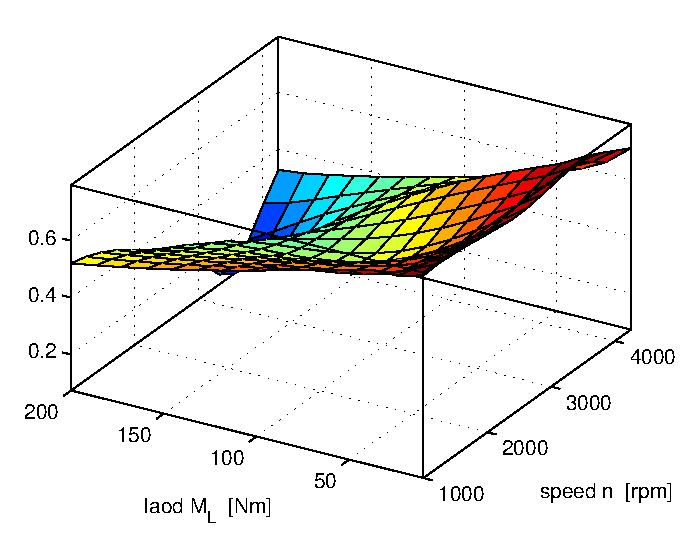
\includegraphics[width=0.75\textwidth]{pics/k_surf.eps}
   \caption{Ein Bild.}
   \label{pics:k_surf}
\end{figure}
\end{verbatim}

\begin{figure}[h]
   \centering
   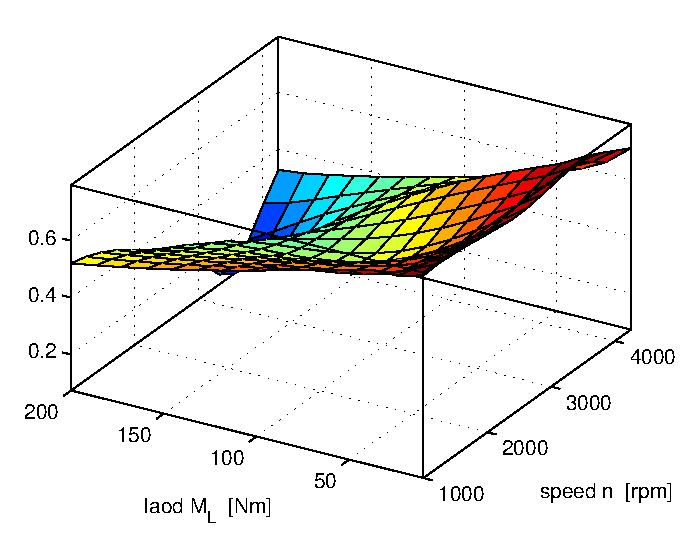
\includegraphics[width=0.75\textwidth]{pics/k_surf.eps}
   \caption{Ein Bild.}
   \label{pics:k_surf}
\end{figure}

oder bei zwei Bildern nebeneinander mit:
\begin{verbatim}
\begin{figure}[h]
  \begin{minipage}[t]{0.48\textwidth}
    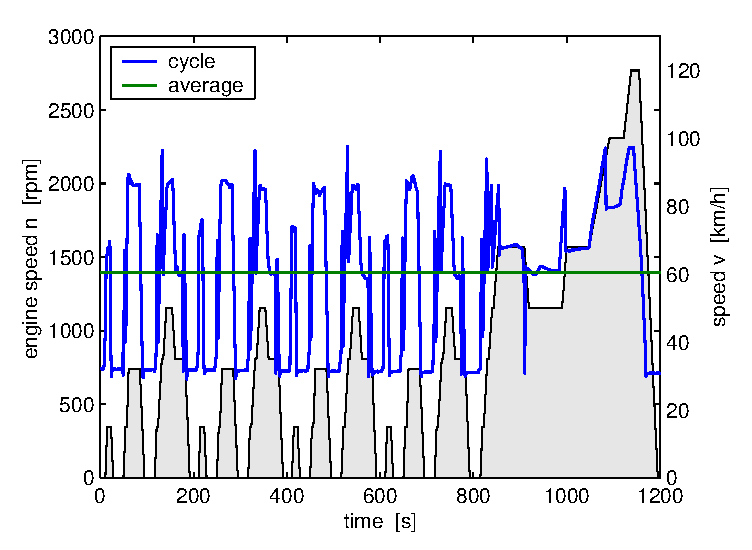
\includegraphics[width = \textwidth]{pics/cycle_we.eps}
  \end{minipage}
  \hfill
  \begin{minipage}[t]{0.48\textwidth}
    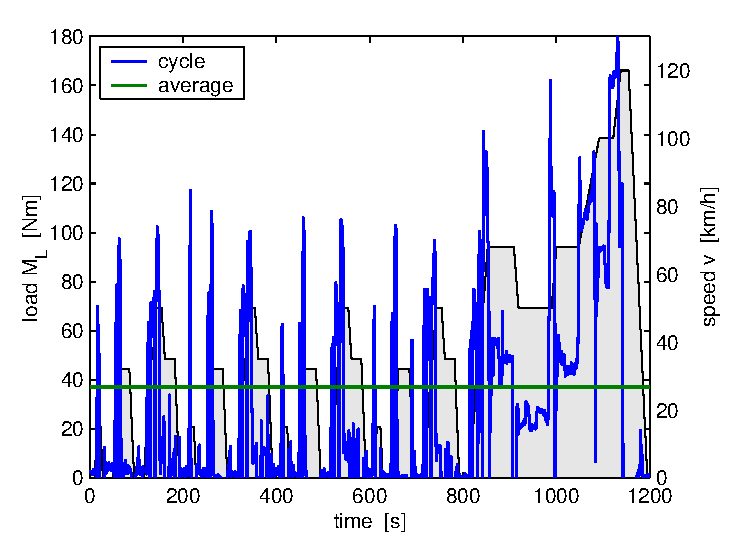
\includegraphics[width = \textwidth]{pics/cycle_ml.eps}
  \end{minipage}
  \caption{Zwei Bilder nebeneinander.}
  \label{pics:cycle}
\end{figure}
\end{verbatim}

\begin{figure}[h]
  \begin{minipage}[t]{0.48\textwidth}
    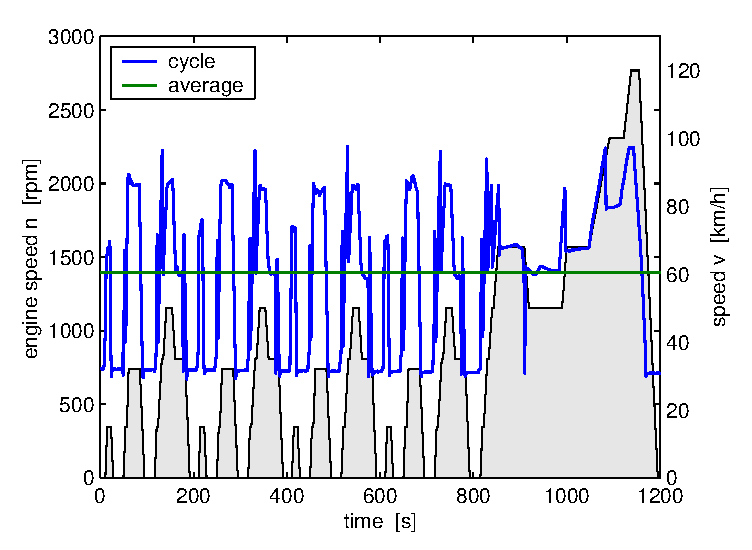
\includegraphics[width = \textwidth]{pics/cycle_we.eps}
  \end{minipage}
  \hfill
  \begin{minipage}[t]{0.48\textwidth}
    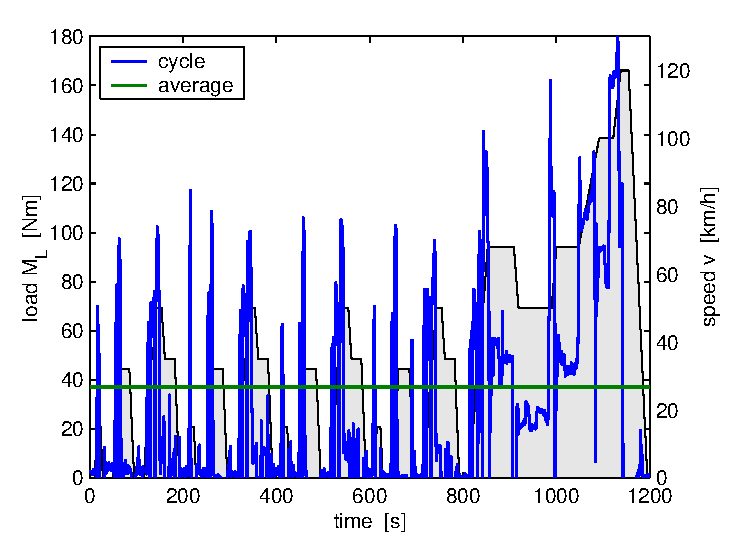
\includegraphics[width = \textwidth]{pics/cycle_ml.eps}
  \end{minipage}
  \caption{Zwei Bilder nebeneinander.}
  \label{pics:cycle}
\end{figure}

Bemerkung: Ersetzt man den Positionierungsparameter \texttt{h}
durch \texttt{H}, so wird das Gleiten der Abbildung verhindert.


\section{Mathematische Formeln}\label{sec:math}

Einfache mathematische Formeln werden mit der equation-Umgebung
erzeugt:
\begin{equation}
 p_{me0f}(T_e,\omega_e) \ = \ k_1(T_e) \cdot (k_2+k_3 S^2
 \omega_e^2) \cdot \Pi_{max} \cdot \sqrt{\frac{k_4}{B}} \, .
\end{equation}

Der Code dazu lautet:
\begin{verbatim}
\begin{equation}
 p_{me0f}(T_e,\omega_e) \ = \ k_1(T_e) \cdot (k_2+k_3 S^2
 \omega_e^2) \cdot \Pi_{max} \cdot \sqrt{\frac{k_4}{B}} \, .
\end{equation}
\end{verbatim}

Mathematische Ausdr�cke im Text werden mit \$formel\$ erzeugt (zB:
$a^2+b^2=c^2$).


\section{Weitere n�tzliche Befehle}\label{sec:div}

Hervorhebungen im Text sehen so aus: \emph{hervorgehoben}. Erzeugt
werden sie mit dem \texttt{\textbackslash epmh\{.\}} Befehl.

% \cleardoublepage
 %!TEX root = Bericht.tex
\chapter{The different Control Modes}
\label{cha:DifferentControlModes}
\section{Elaboration}
\label{sec:elaboration}
\textit{About the need of different modes, the requirements of image capturing and overview of the realized modes}
\section{Manual Control Modes}
\label{manualControlModes}
\textit{Direct Control and Assisted Control}
\section{Automatic Control Modes}
\label{automaticControlModes}
\textit{Half Automatic Control and Full Automatic Control}
 \cleardoublepage
 %!TEX root = Bericht.tex
\graphicspath{{graphics/HMI/}{graphics/control_modes/}}
\chapter{Finding a Hardware and Software Solution}
\label{cha:findHardSoftSolution}
In the following it is described how the previously defined control modes were realized and what else lead to the finally realized HMI which is described in section \ref{sec:realization}. On the one hand there was the hardware which had to be chosen and on the other hand the software to realize the control modes with that hardware had to be written.



\section{Requirements}
\label{sec:requirements}
One of the goals of this bachelor thesis was to develop a HMI which was tailored to \textsc{Skye}. In the following listing, all requirements demanded for such a HMI are pointed out: \\

The hardware used for the HMI should...
\begin{itemize}
\item[...]{offer intuitive control for six DOF, i.e. fit the defined control modes, }
\item[...]{be portable,}
\item[...]{offer wireless connection, i.e. ports for attaching a \textsc{XBee} module and a Wi-Fi router,}
\item[...]{be able to display the video stream of \textsc{Skye},}
\item[...]{offer the possibility to set waypoints for \textsc{Skye},}
\end{itemize}
whereas the used operation system should be compatible with the driver of the \textsc{XBee} module and with \textsc{ROS}\footnote{The decision to use a \textsc{XBee} module and Wi-Fi for communication is explained in \cite{burri}. There it is also explained how \textsc{ROS} is used to process imagery. Detailed description about \textsc{ROS}, the Robot Operating System, can be found on \url{http://www.ros.org/wiki/}.}.

\section{Existing Solutions}
\label{sec:existingSolutions}
Existing HMI solutions were analyzed in order to find out, whether they would be convenient to adopt and whether they would fulfill the requirements on their own. 

\subsection{Hardware}
\label{sub:hardware}

Figure \ref{fig:devices taken into consideration} shows all devices which were taken into closer consideration. The gamepad option was drapped as it would offer the same possibilities as RC does with the drawback of not being a stand alone device. Smartphones could not be used as they run with operation systems not compatible with \textsc{ROS}.

\begin{figure}[h]		
	\small{
		\begin{center}
			\parbox[b]{0.25\textwidth}{\includegraphics[width=0.25\textwidth]{futaba_7C_radio_encircled}
			\begin{center}RC \end{center}}
			\hspace{0.05\textwidth}
			\parbox[b]{0.25\textwidth}{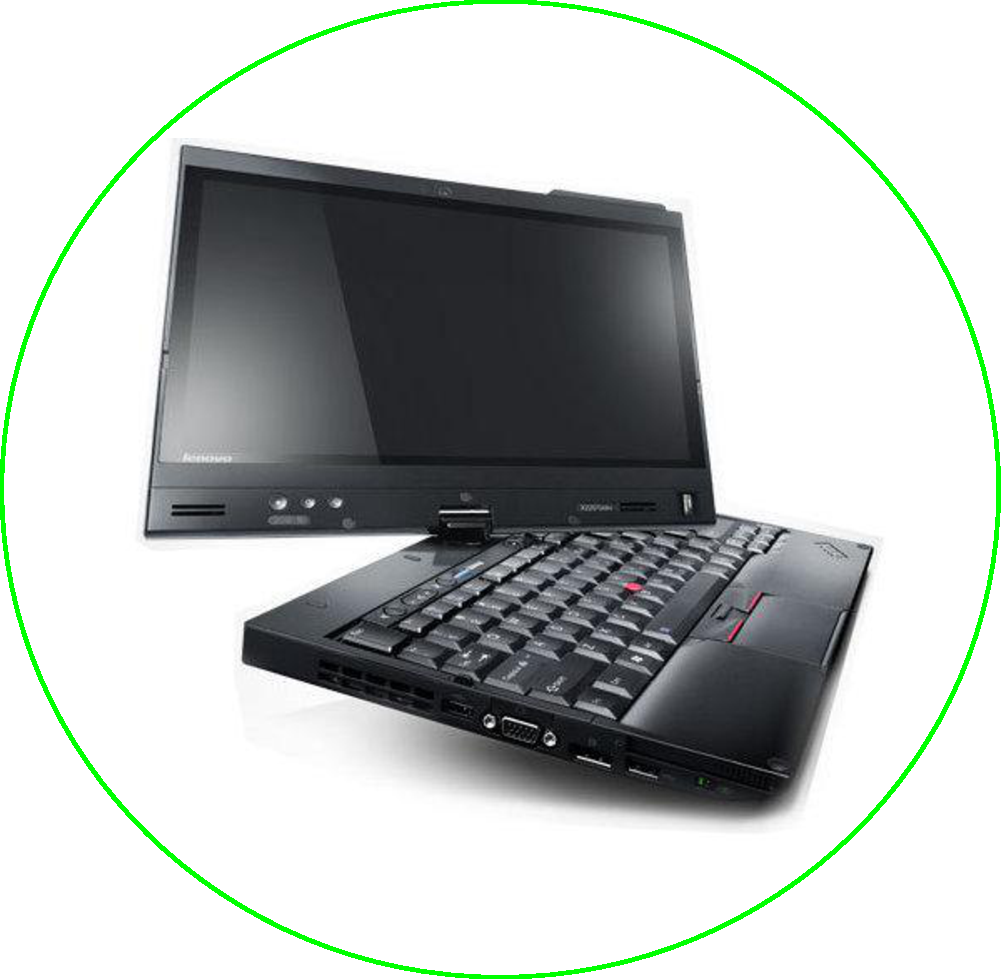
\includegraphics[width=0.25\textwidth]{x220t_hero_encircled}
			\begin{center}Tablet \end{center}}
			\hspace{0.05 \textwidth}
			\parbox[b]{0.28\textwidth}{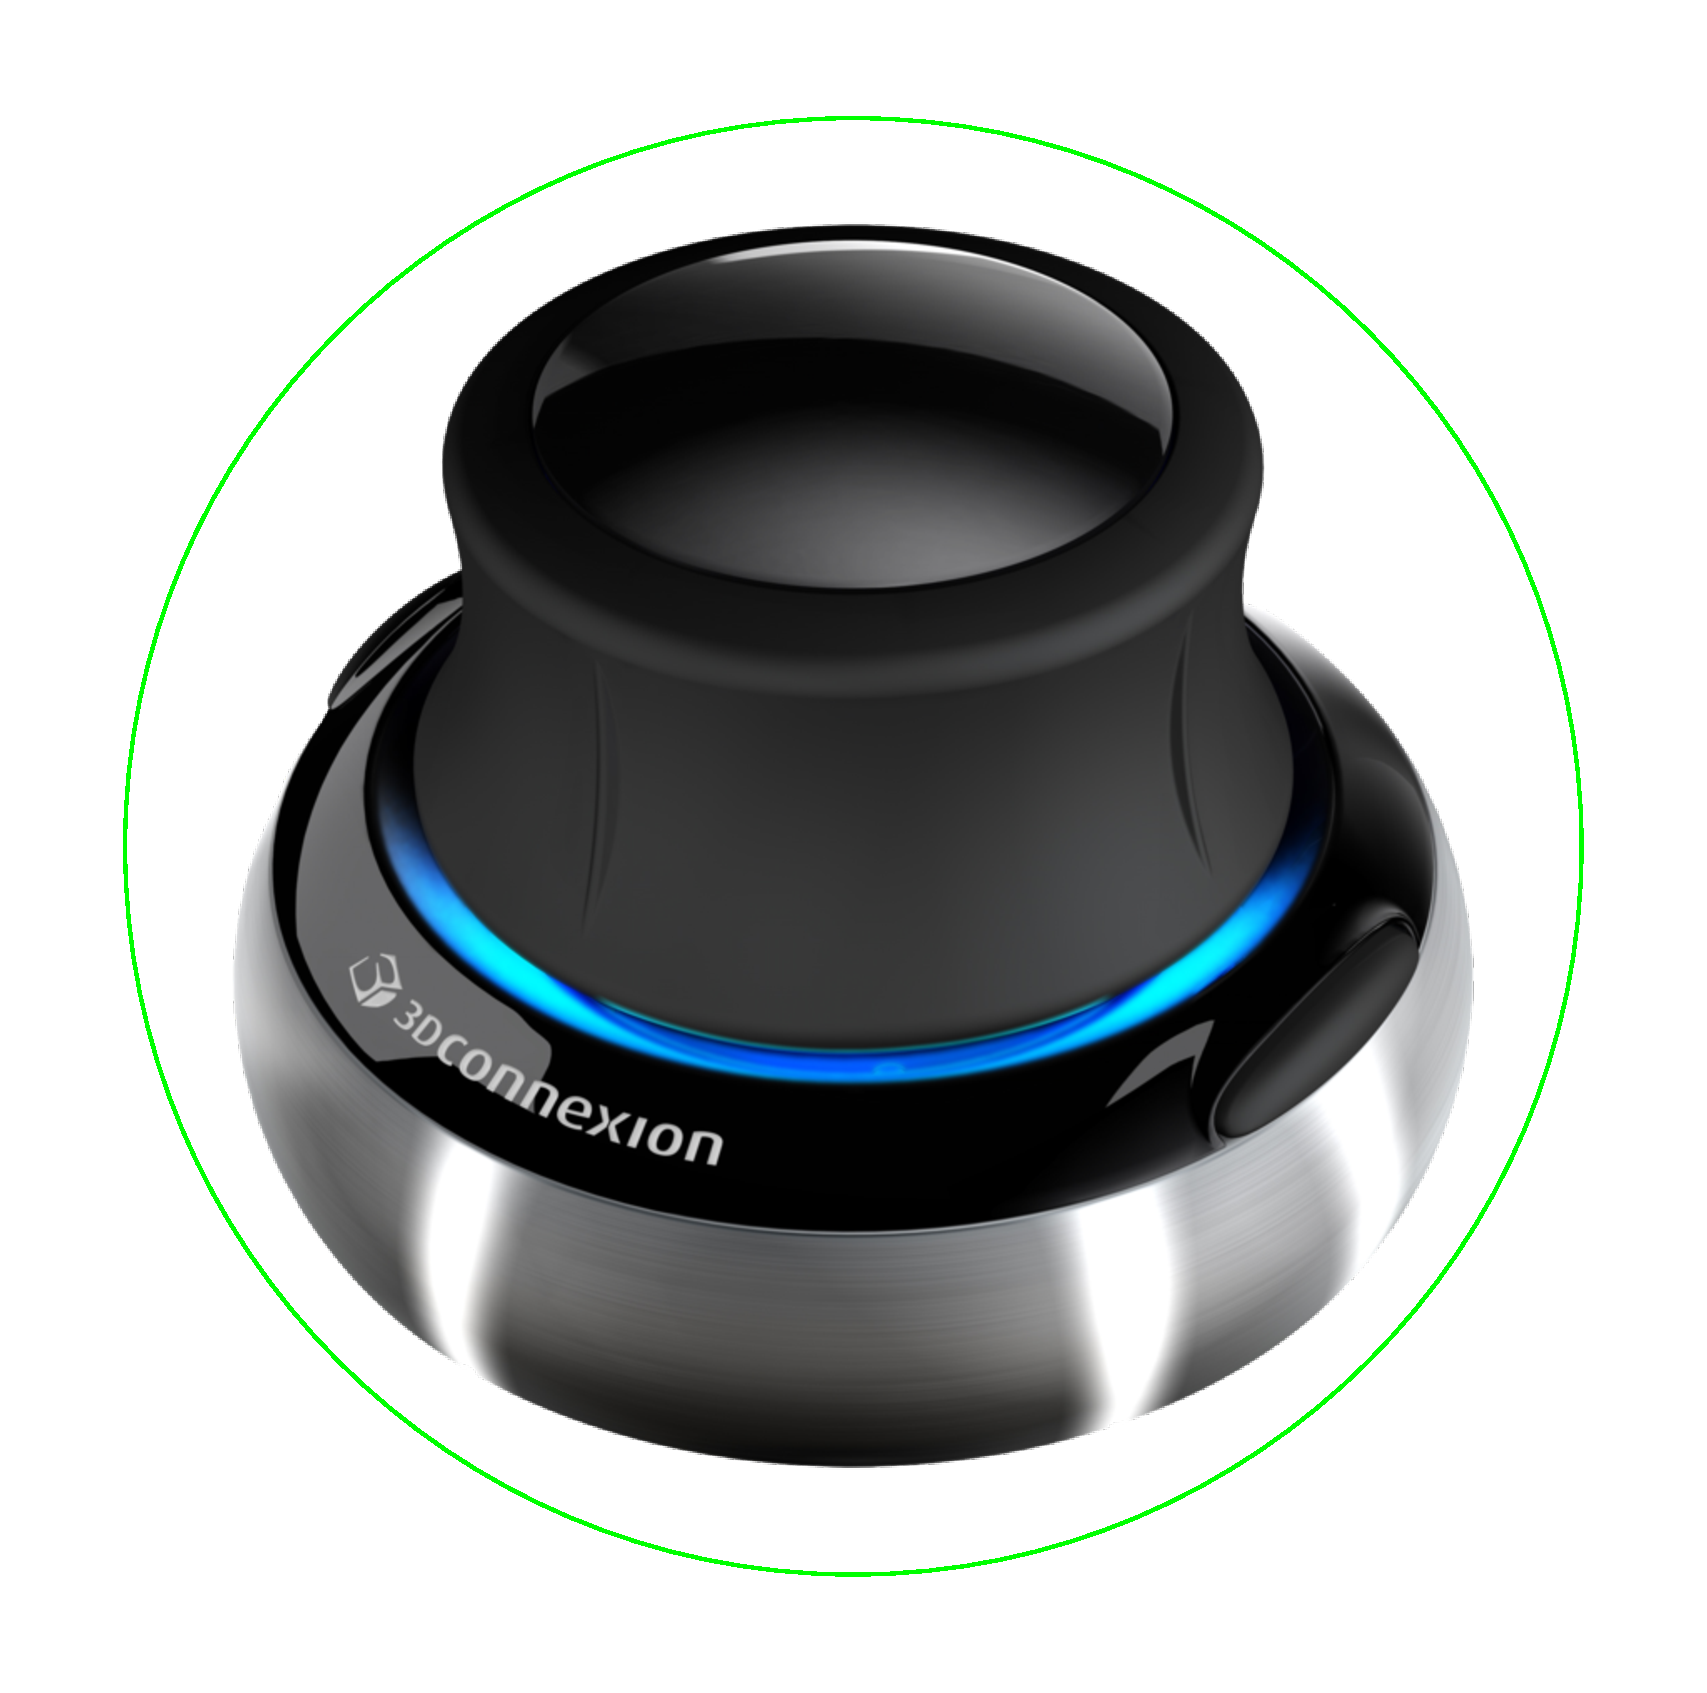
\includegraphics[width=0.28\textwidth]{3dx_productimage_encircled}
			\begin{center}3D mouse \end{center}}			
			\vspace{0.005\textwidth}
			\hspace{0.05\textwidth}			
			\parbox[b]{0.25\textwidth}{
\includegraphics[width=0.25\textwidth]{qgo_sphere_cut}
			\begin{center}Qgo Sphere \end{center}}
			\hspace{0.05\textwidth}
			\parbox[b]{0.25\textwidth}{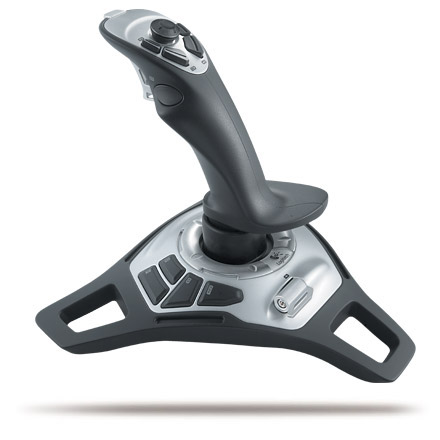
\includegraphics[width=0.25\textwidth]{Logitech-Freedom-Cordless-Joystick}
			\begin{center}Joystick \end{center}}
			\caption{The considered devices whereas the tablet with attached 3D mouse finally was chosen. The RC serves as a backup.}
			\label{fig:devices taken into consideration}	
		\end{center}
	}			
	\vspace{4.5mm}
\end{figure}

Table \ref{tab:requirements and expectations for hardware} shows the rating of the considered devices. It is visible that a solution in combination with a tablet had to be used, as only a tablet is able to fulfill the criteria for automatic controls and to run \textsc{ROS}. Although the Qgo Sphere\footnote{In  \cite{kammermann} the usage of the Qgo Sphere as an input device for a ballbot is discussed.} would be most intuitive to use with \textsc{Skye}, a 3D mouse (a space navigator from \textsc{3DConnection}) was chosen as a supplementary device to the tablet. Because of the fix-installed infrared sensors needed for the detection of the sphere's translational movements, the Qgo Sphere is not portable, which made it inconvenient to use for \textsc{Skye}. A joystick is not designed for six DOF and is therefore much less intuitive in use as a 3D mouse. For the tablet a \textsc{Lenovo} X220 was chosen as it can be transformed to a common notebook. This allows easy postprocessing of any gathered data. Additionally, a \textsc{Futaba} 7C RC serves as a backup in case of any breakdown within the main HMI.


\begin{table}[H]		% [H] indicates that the table should be right here.
	%\begin{tabularx}{\textwidth}{p{0.125\textwidth}p{0.2\textwidth}|p{0.06\textwidth}p{0.075\textwidth}p{0.08\textwidth}p{0.1\textwidth}p{0.08\textwidth}}	% add p{size_of_colomn} for every new column you'd like to have. If you put a | between the p then there is a vertical line between the columns. 
	\begin{center}
 \begin{tabular}{ll|ccccc}
\multicolumn{2}{l|}{Device}	& \rotatebox{90}{\mbox{RC}} 	& \rotatebox{90}{\mbox{Tablet}} 	&\rotatebox{90}{\mbox{3D Mouse}}	&\rotatebox{90}{\mbox{Qgo Sphere}}	&\rotatebox{90}{\mbox{Joystick}}  \\
	\toprule[1.25pt]				%define the line thickness of the top rule
	\multicolumn{2}{l|}{Stand alone}							&$\checkmark$		&$\checkmark$		&-			&-			&-\\
	\hline%\midrule
	\multirow{5}{*}{Matching}		&Test Phase					&-				&$\checkmark$		&-			&-			&-\\
									&Direct Control				&$\checkmark$		&$\checkmark$		&$\checkmark$	&$\checkmark$	&$\checkmark$ \\
									&Assisted Control			&$\checkmark$		&$\checkmark$		&$\checkmark$	&$\checkmark$	&$\checkmark$ \\
									&Half Automatic Control		&-				&$\checkmark$		&-			&-			&- \\
									&Full Automatic Control		&-				&$\checkmark$		&-			&-			&-\\
	
	\hline%\midrule
	\multicolumn{2}{l|}{Live View}							&-				&$\checkmark$		&-			&-			&-\\
	\hline%\midrule
	\multicolumn{2}{l|}{Intuitive}								&quite	&quite	&very&most&quite\\
	\hline%\midrule
	\multicolumn{2}{l|}{Portable}								&most	&quite	&quite&not &quite\\
		
	\bottomrule[1.25pt]
	%\end{tabularx} 
	\end{tabular}
	\caption[Requirements and Expectations for the Hardware]{Requirements and Expectations for the Hardware}
	\label{tab:requirements and expectations for hardware}
	\end{center}
\end{table}


\subsection{Software}
%\textit{QGroundControl, OpenPilot, Qt-Libraries} \\
\textsc{Google} and \textsc{Apple} showed how intuitive a GUI can be in combination with a  touchscreen with their operating systems for smartphones. They offer the user unknown flexibility in adopting the GUI to his needs. However, out of \textsc{Windows}, \textsc{Ubuntu}, \textsc{Mac OS}, \textsc{iOS} and \textsc{Android}, \textsc{Ubuntu} was the only operating system which provides complete support for \textsc{ROS}. Therefore \textsc{Ubuntu 11.10} was chosen as the operating system for the tablet.\\
As it was clear that there was no GUI ready to use unchanged for the HMI, open source software was analyzed in order to adopt it for \textsc{Skye}. Using \textsc{QGroundControl} (described in section \ref{subsec:qGroundControl}) was the best option. On the one hand it already offered the commonly used tools to control a UAV and on the other hand a good support in adopting it to the needs of \textsc{Skye} was granted as it was developed at the \textsc{ETH}.


\section{Realization}
\label{sec:realization}

\subsection{Compact and Convenient Solution}
Using a 3D mouse in combination with a tablet computer has a lot of advantages. Both devices can be put on a board with suspenders. Like this, the pilot has a compact portable control unit, without any external hardware interconnected (compare figure \ref{fig:HMI_in_Action}). While the 3D mouse provides intuitive control of the six DOF, the tablet with its GUI is used to filter and route the signals of the 3D mouse or serves as a highly modular touch input device on its own. With \textsc{QGroundControl} running on it, it also enables the pilot to adjust the controller and to set waypoints, while during the whole flight the live view of \textsc{Skye} is displayed (More on that in section \ref{subsec:qGroundControl}). In case the tablet should crash, the RC can be used to bring down \textsc{Skye} safely to ground.

\begin{figure}[H]
	\begin{center}
		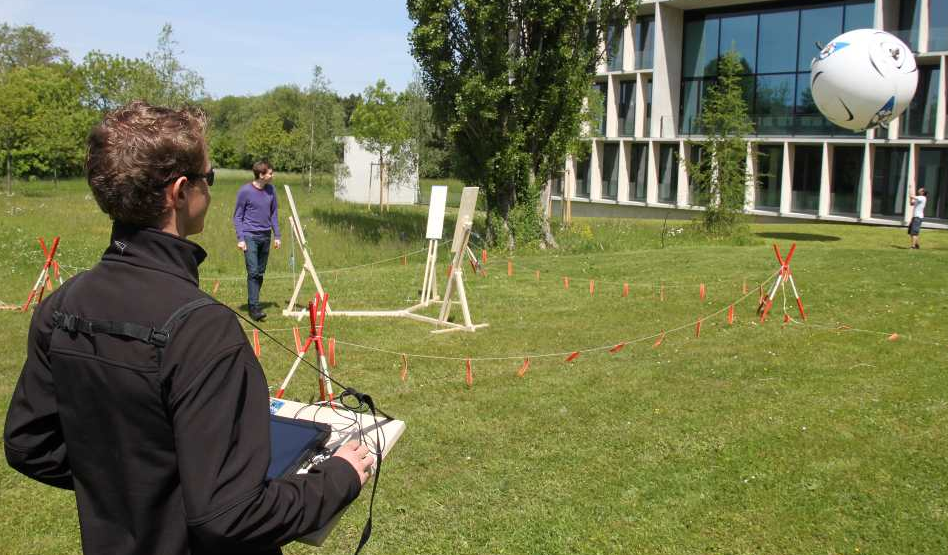
\includegraphics[width=0.85\textwidth]{graphics/HMI_in_Action}
		\caption{The compact, portable control unit in action}  
		\label{fig:HMI_in_Action}
	\end{center}
\end{figure}



\subsection{QGroundControl}
\label{subsec:qGroundControl}
%\textit{Adaptions in QGroundControl, 3dMouse, Touchscreen, Splines and Trajectory Controller \\ Only how it looks like and how to use. All ``important'' widgets are shown in detail. Implementation of 3dMouse and Touchscreen are not described further.picture of touch in action, mail final presentation}

The GUI \textsc{QGroundControl} for controlling unmanned vehicles was initially developed for \textsc{Pixhawk}\footnote{For more information on this project, see \url{https://pixhawk.ethz.ch/}.}, a vision based UAV project at the informatics department of \textsc{ETH}. It is a complete open source project based on Qt, which is a cross-platform-framework for GUIs written in \verb!C++!. For this thesis, the complete \textsc{QGroundControl} source code was taken and adopted for the needs of project \textsc{Skye}. This varied from adding single lines to develop complete new additional widgets\footnote{Widgets are kind of subwindows of the application.}. These widgets are described below. Inspiration and know-how was taken from \cite{blanchette} and nice tutorials and samples on \url{http://qt.nokia.com/}. In the following it is explained, how the control modes, defined in chapter \ref{cha:DifferentControlModes}, were realized with the chosen devices and with the GUI \textsc{QGroundControl}\footnote{The \textit{full automatic control} mode was only simulated in \textsc{Matlab} and therefore no support of the GUI exists.}. 
\\
%\textbf{HERE matthias would like to summarize the basic code structure of qgc.. so it can be refered to and from the \textsc{Mavlink} section} 
%\\
To allow full control of system \textsc{skye}, a derived subclass to handle system specific procedures had to be programmed. 
This had to be done within compatibility to the messages defined in the \textsc{Mavlink} protocol (see section \ref{subsec:mavlink}). Precompiler commands have been used for cross-platform compatibility and \textsc{Skye} system specifications. 
With the Qt specific signals/slots interface the \textsc{Skye} subclass has been connected with the communication link as well as the user interfaces. 
An event handler has been integrated using the 3DxWare API, the official development kit for the used 3D mouse.

\subsubsection{The Main Control Widget}
With five different control modes (\textit{test phase}, \textit{direct control} (DC), \textit{assisted control} (AC), \textit{half automatic control} (HAC), \textit{full automatic control} (FAC)) and three different input option (3D mouse, touchscreen, keyboard), a main control widget was needed to choose between these options (see figure \ref{fig:qgc_skye_control} for its appearance). 
%With it the pilot can choose the control mode\footnote{As the Test Phase is not a usual control mode, its widget has to be opened in the menu bar.} and the input option.
The \textit{test phase} mode is not meant to be used in flight and has therefore be activated via the menu bar.
The two sliders visible in figure \ref{fig:qgc_skye_control} allow to adjust the input scaling for translations and rotations respectively. Indoor flights need usually smaller but more accurate inputs, while outdoors more power is needed. The colored arm/disarm button is used to (de-)activate the actuators. At the same time it serves as an emergency button.

\begin{figure}[H] % [H] steht dafür, dass das Bild genau hier im Text sein soll.
	\begin{center}
		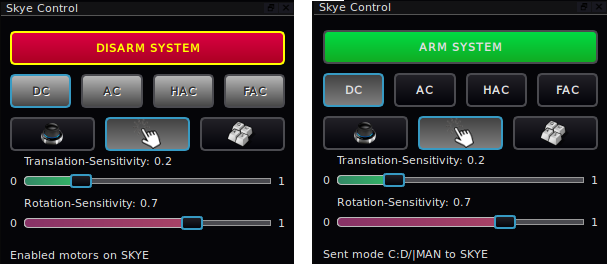
\includegraphics[width=0.7\textwidth]{qgc_skye_control}
		\caption{The main control widget in which most modes and options can be set. On the right its appearance with activated actuators and and the left its appearance with deactivated actuators.}
		\label{fig:qgc_skye_control}		
	\end{center}
\end{figure}



\subsubsection{Test Phase Control}
In order to test \textsc{Skye}'s four actuators before flight and in the development process, another widget was developed. It allows to adjust each of the eight actuation inputs separately. The input for the four thrusters is set by sliders and the orientation is set by turning the knobs. Again, there is a main button (Activate Engine) to start and stop the motors.

\begin{figure}[H] % [H] steht dafür, dass das Bild genau hier im Text sein soll.
	\begin{center}
		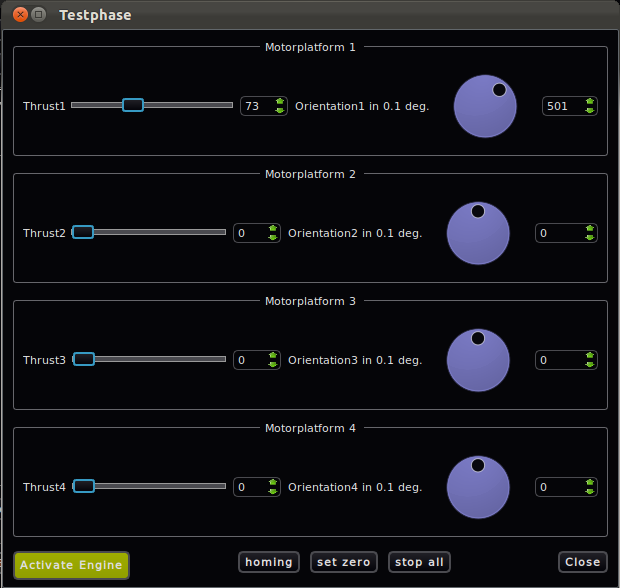
\includegraphics[width=0.7\textwidth]{qgc_test_phase}
		\caption{The \textit{test phase} widget }  
		\label{figure:qgc_test_phase}
	\end{center}
\end{figure}


\subsubsection{Direct Control}
The main device for the \textit{direct control} mode is the 3D mouse which is connected by USB to the tablet. To use its input signals in  \textsc{QGroundControl}, a interface had to be written. With the two knobs on the device (hardly visible in figure \ref{fig:3D_mouse}) the pilot is able to (de-)activate translational or rotational inputs. This allows a very precise control.

\begin{figure}[H] % [H] steht dafür, dass das Bild genau hier im Text sein soll.
	\begin{center}
		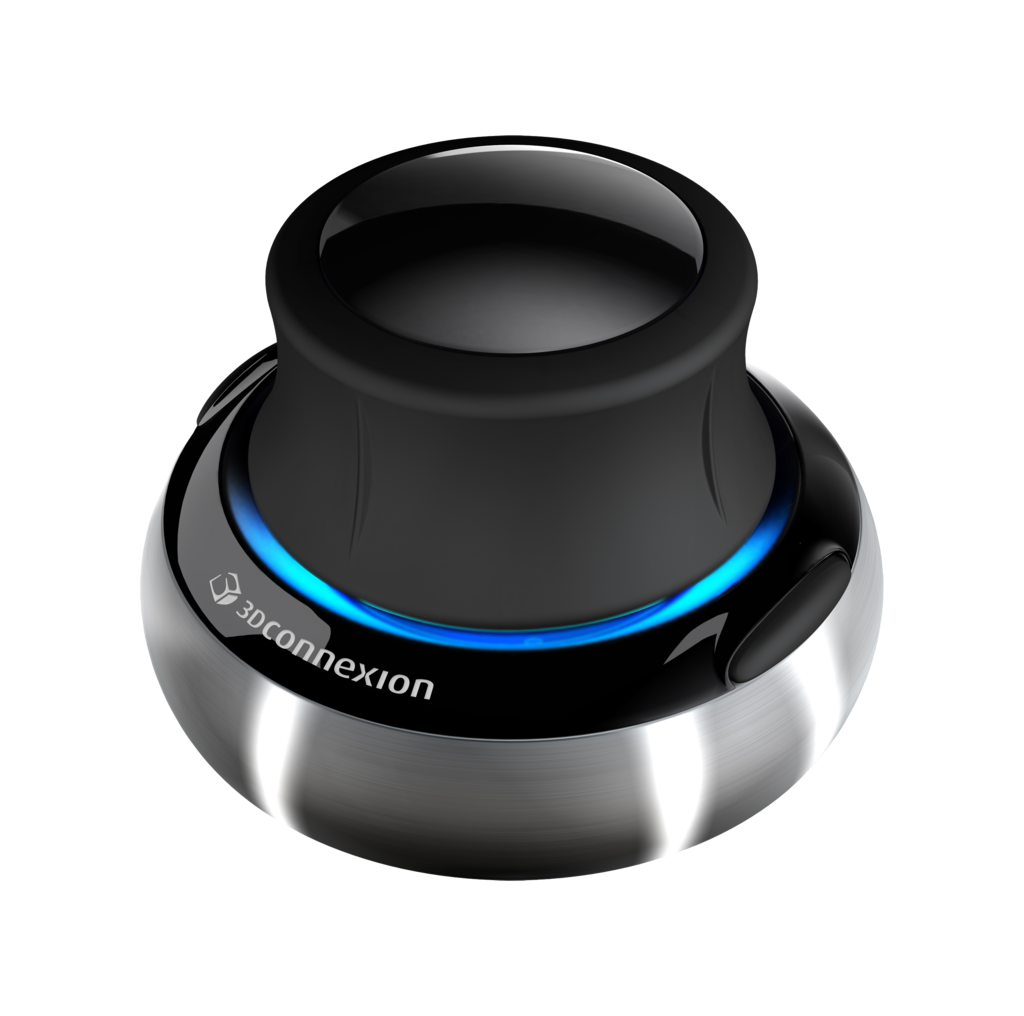
\includegraphics[width=0.4\textwidth]{3dx_productimage}
		\caption{The 3D mouse used for the \textit{direct control}}  
		\label{fig:3D_mouse}
	\end{center}
\end{figure}

\subsubsection{Assisted Control}
\label{subsub:assistedcontrol}
Feeding velocities instead of a force and a moment makes the usage of the touchscreen beside the 3D mouse more reasonable. For this mode a combination of different widgets is used, shown in figure\footnote{This screenshot is a reproduced situation of the flight in ETH main building. Obviously, no GPS information were available then.} \ref{fig:qgc_manual_control}. The widgets can be scaled and positioned individually. As a default view for \textsc{Skye}, the shown arrangement of the Head-up-Display (HUD), map and main control widget is provided. If touch input is chosen, the HUD enables rotational touch inputs directly on the displayed live view. The map widget shows the position of \textsc{Skye} and allows to set translational inputs. Note that in a first approach these inputs were always interpreted in the camera frame as the state estimation was not yet running. Intuitively, this has to be transformed to inputs in the North-East-Down (NED) frame which has recently been tested on the system.

\begin{figure}[H] % [H] steht dafür, dass das Bild genau hier im Text sein soll.
	\begin{center}
		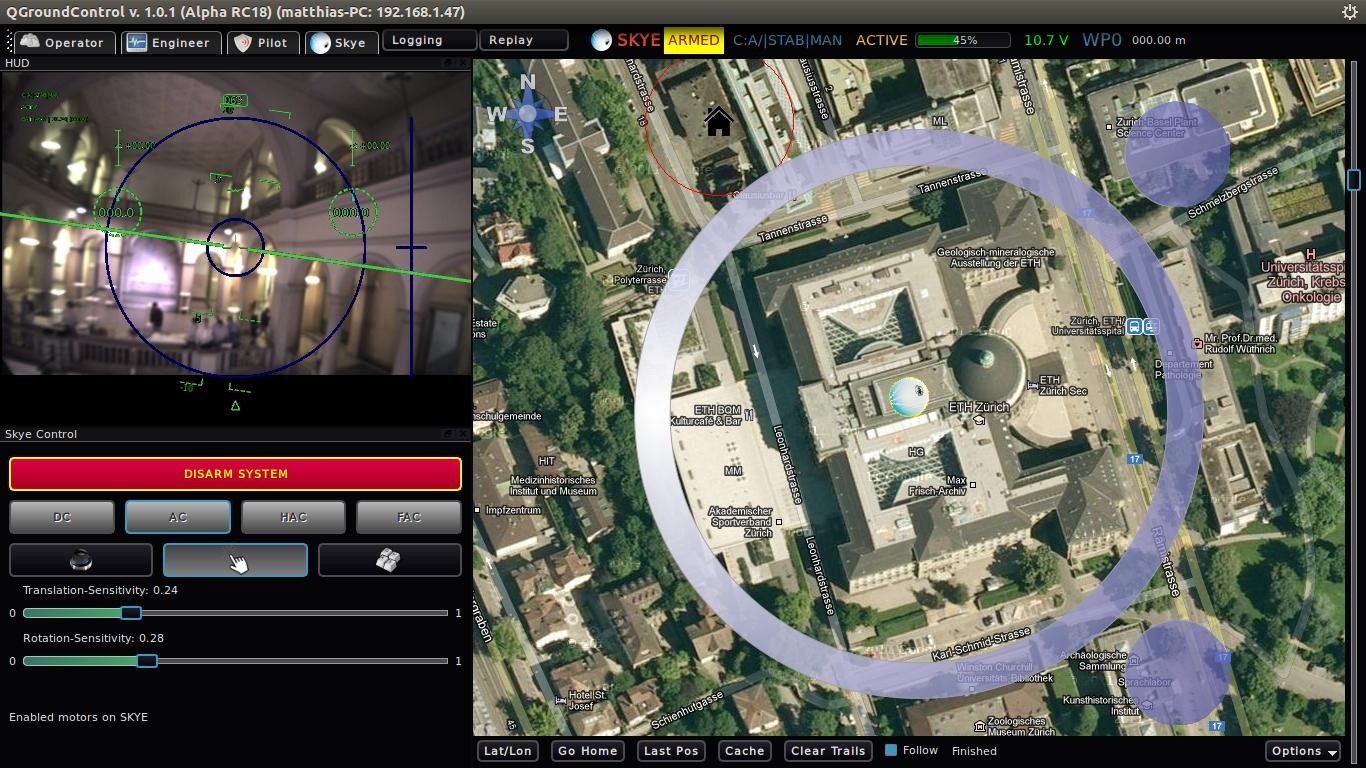
\includegraphics[width=0.8\textwidth]{qgc_manual_control}
		\caption{The pilot's view on the GUI if assisted  control and touch input is activated.}  
		\label{fig:qgc_manual_control}		
	\end{center}
\end{figure}

\begin{figure}[H] % [H] steht dafür, dass das Bild genau hier im Text sein soll.
	\begin{center}
		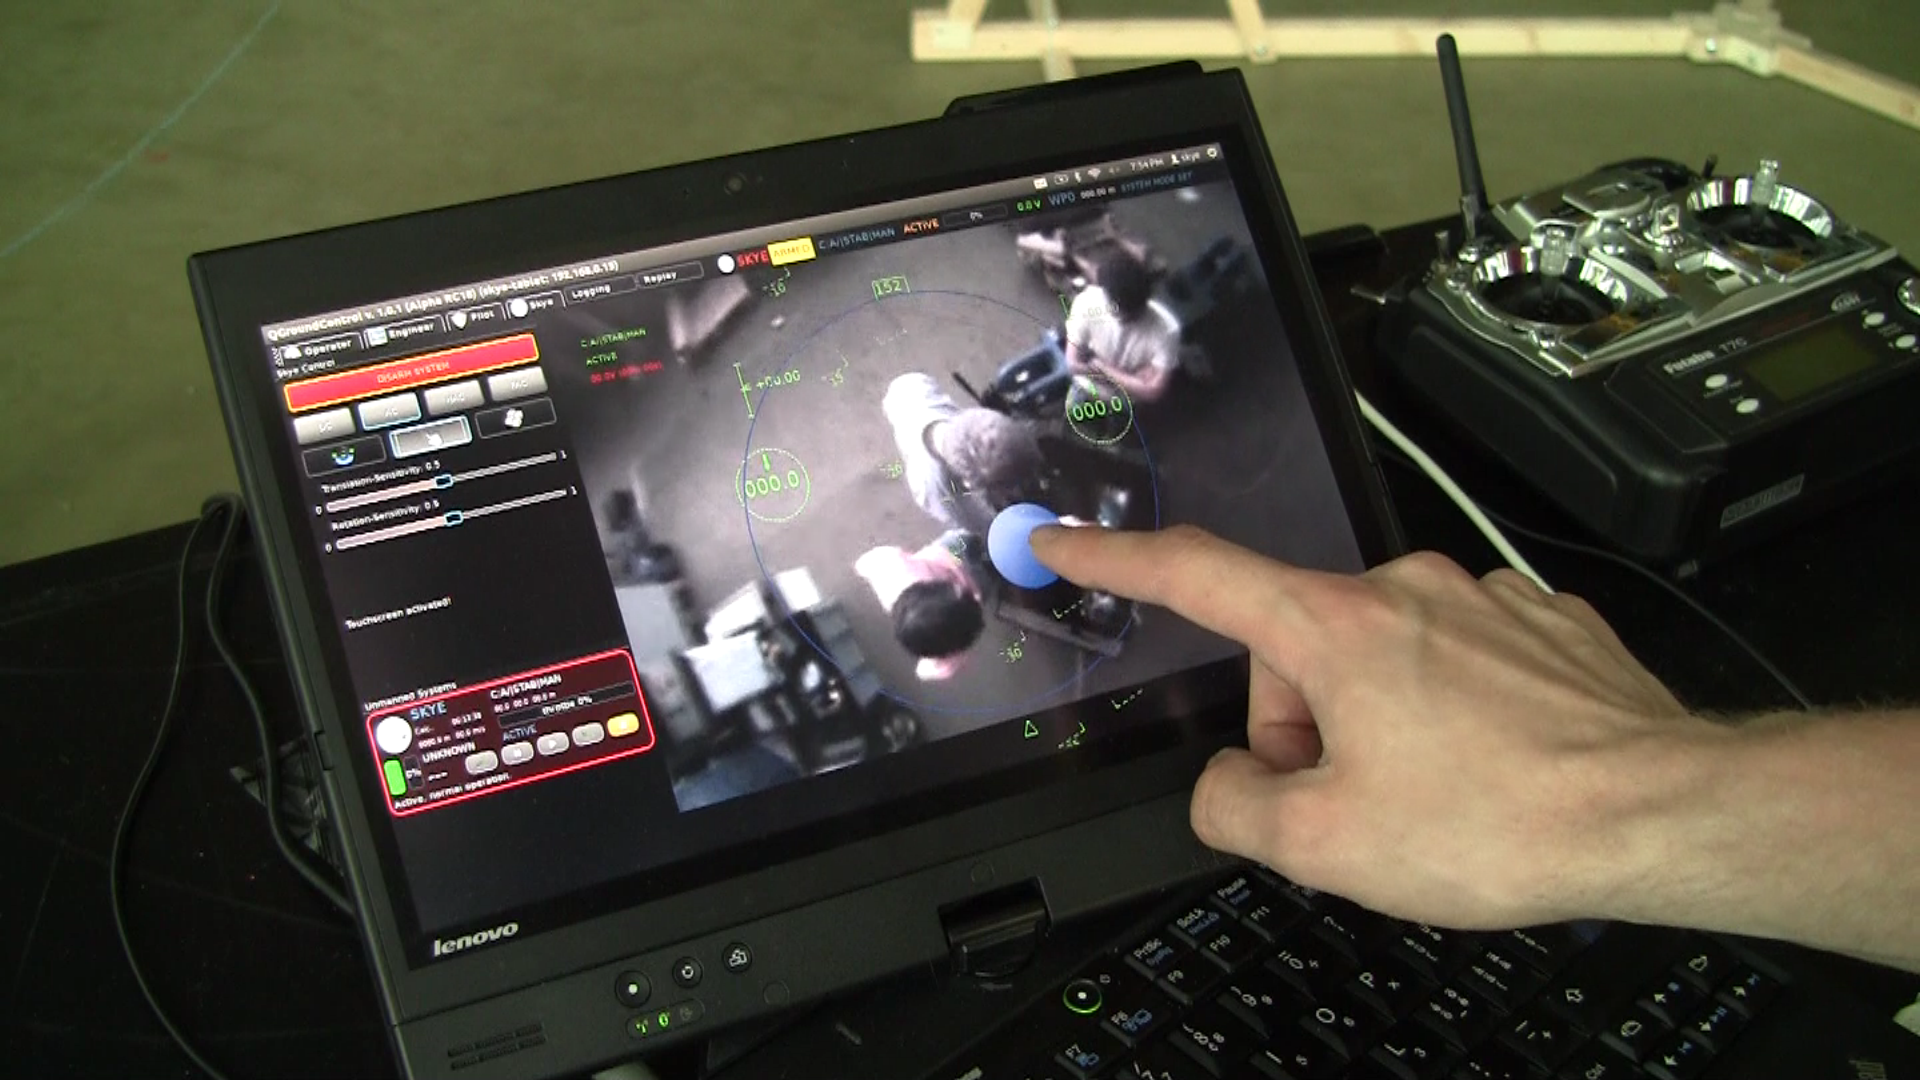
\includegraphics[width=0.8\textwidth]{graphics/TouchInput}
		\caption{The enlarged HUD with touch input in action}  
		\label{fig:touchInput}		
	\end{center}
\end{figure}


\subsubsection{Half Automatic Control}
\label{subsub:halfautomaticcontrol}
For this mode a trajectory is needed. Therefore \textsc{QGroundControl} was adopted to generate it. After setting the waypoints on Google Maps, the user can adjust the their height over ground. In order to properly display the elevation, the Google Elevation API\footnote{\url{https://developers.google.com/maps/documentation/elevation/}}was used. Once the waypoints are set an interpolating cubic spline is calculated and displayed (see figure \ref{fig:qgc_automatic_control}). Out from the recent position of \textsc{Skye}, a velocity input is calculated using a \textit{Pure Pursuit} approach\footnote{In section \ref{sub:pure_pursuit} \textit{Pure Pursuit} is described how it was implemented in \textsc{Matlab}.} The part of the path that is already reached is displayed in blue. The methods for waypoint interpolation and trajectory generation are describe in more detail in chapter \ref{cha:trajectory}.% The trace of the (simulated) motion is tracked with red dots.

\begin{figure}[H] % [H] steht dafür, dass das Bild genau hier im Text sein soll.
	\begin{center}
		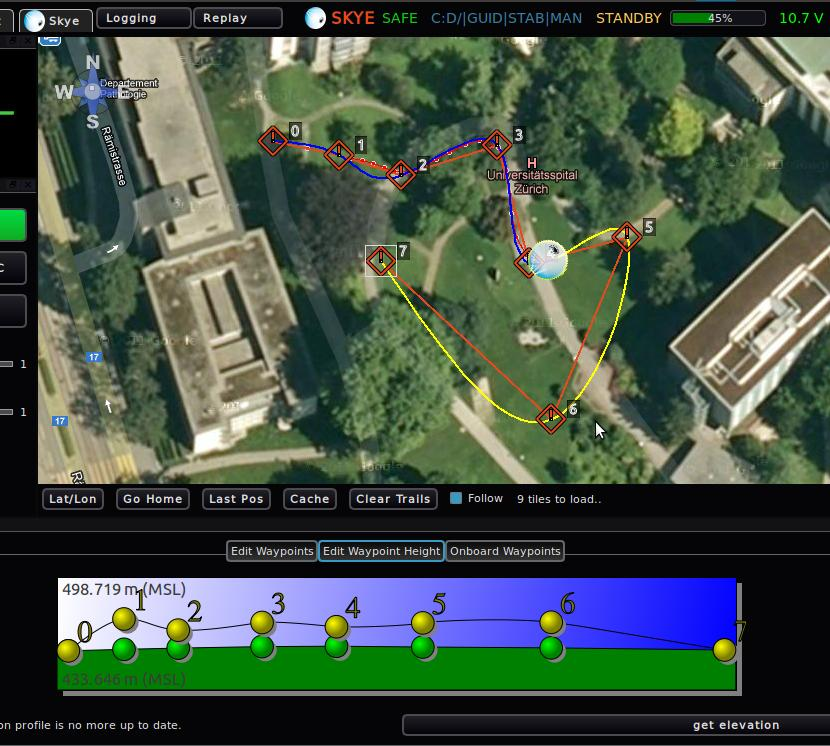
\includegraphics[width=0.8\textwidth]{qgc_automatic_control}
		\caption{Generating a trajectory with the GUI}
		\label{fig:qgc_automatic_control}		
	\end{center}
\end{figure}

%\textbf{A Picture of the DC/AC widget should be placed at least in the APENDIX.. Camera reconfiguration and battery info can be left away.}

Further on, widgets to adjust camera properties, displaying detailed battery info or to set \textit{direct} or \textit{assisted control} to exact values via sliders have been added. Despite of the latter\footnote{The \textit{direct} and \textit{assisted control} widget has been used to enable the system verifications in \cite{meiermueri} and \cite{weichart}.} they could not be used in practice. The \textit{direct} and \textit{assisted control} widget is shown in figure \ref{fig:qgc_manual_control_widget}.

\subsection{Mavlink}
\label{subsec:mavlink}
%\textit{Summary of Protocal, adaptions and use for} \textsc{Skye} \\
Mavlink (Micro Air Vehicle Communication Protocol) is a very lightway header-only message marshalling library for micro air vehicles\footnote{Official description from \url{http://qgroundcontrol.org/mavlink/start}}. It is a widely used protocol geared for transmission speed and safety. A mavlink packet consists of a six byte prefix including start byte, payload length and sequence number as well as component, system and message ID. A two byte suffix checksum is used. The payload size is maximum 255 bytes. Many autopilots as well as cross-platform software packages are using Mavlink.
A set of commonly used messages is provided. The protocol had to be extended for the convenient use with \textsc{Skye} (an example
%\footnote{The full xml file including the message definitions for \textsc{Skye} is in the appendix (listing \ref{app_xml}).}
 of such a message definition is shown in listing \ref{xml_assisted_control}). This can be done by defining the additional messages in a xml script. The C-headers will be generated by the Mavlink Generator. The control commands, system telemetry as well as image live stream for \textsc{Skye} are transmitted using Mavlink protocol. For the transmission of waypoints, an extended waypoint protocol is provided by Mavlink. The waypoints set on the map widget and height profile (see section \ref{subsub:halfautomaticcontrol}) as well as the autopilot (\textit{PX4FMU}) are compatible to this protocol.

\begin{figure}
\begin{lstlisting}[captionpos=b, caption=Sequence of skye.xml: Definition of the Assisted Control command Mavlink message. It consists of six 32 bit floating numbers for the input values and a 8 bit integer to indicate the target system's ID (the GUI could actually be connected to more than one UAV at the same time)., label=xml_assisted_control]
<message id="155" name="SKYE_ASSISTED_CONTROL">
   <description>Control six degrees of freedom. Translational velocity in Inertial (earth) Frame. Use this manual control mode with the requested mode: 
"MAV_MODE_ASSISTED_CONTROL_ARMED"</description>
   <field type="uint8_t" name="target_system">System ID</field>
   <field type="float" name="translation_lat">Translation (velocity) in Inertial Frame latitude, in m/sec</field>
   <field type="float" name="translation_long">Translation (velocity) in Inertial Frame longitude, in m/sec</field>
   <field type="float" name="translation_alt">Translation (velocity) in Inertial Frame altitude, in m/sec</field>
   <field type="float" name="rotation_x">Roll (angular velocity), in rad/sec</field>
   <field type="float" name="rotation_y">Pitch (angular velocity), in rad/sec</field>
   <field type="float" name="rotation_z">Yaw (angular velocity), in rad/sec</field>
</message>
\end{lstlisting}
\end{figure}

 \cleardoublepage
 %!TEX root = Bericht.tex
\graphicspath{{graphics/}{graphics/controller/}}

\chapter{Trajectory Planning}
\label{cha:trajectory}
For the two most advanced modes, i.e. the \textit{half automatic} and the \textit{full automatic} mode described in chapter \ref{cha:DifferentControlModes}, trajectories have to be generated. In this chapter the best trajectories for \textsc{Skye} are elaborated and tested with suitable trajectory controllers. Performance results based on a \textsc{Matlab} simulation are shown.

%\subsection{Our Approach}
%From the GUI it was given that the goal trajectory would be a multipoint-interpolating %trajectory. The user is able to define waypoints on a map which afterwards should be %connected with a reasonable and realizable trajectory. Beside interpolating trajectories %there exist also approximating trajectories but they were not taken into consideration, since %usually the user wants skye fly directly through a waypoint.

\section{Experimental Design}
\label{sec:experimental design}
The main application fields of the system \textsc{Skye} are image capturing and agile performance demonstrations. The waypoints used to test the trajectory algorithms have therefore to be alike these situations. All the results in this chapter belong to the three sample waypoints shown in figure \ref{fig:sampleNodes}. The first waypoints e.g. could be used to capture images of the university building. Generally spoken, they represent standard situations for the applications mentioned before. Indeed, to verify the conclusions, sometimes a wider set of waypoints had to be considered. 

\begin{figure}[h]
  \begin{minipage}[t]{0.32\textwidth}
    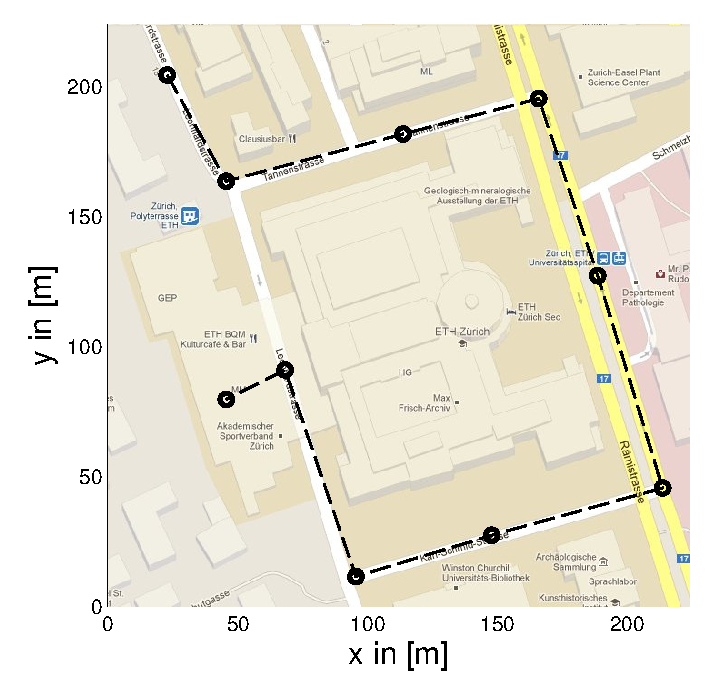
\includegraphics[width = \textwidth]{graphics/sampleNodeRoad}
  \end{minipage}
  \hfill
  \begin{minipage}[t]{0.32\textwidth}
    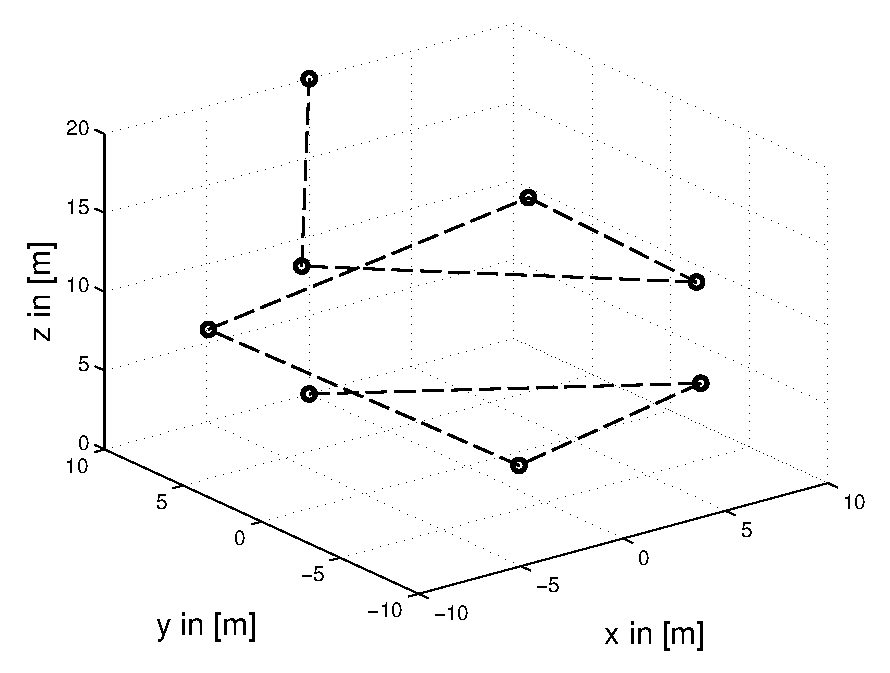
\includegraphics[width = \textwidth]{graphics/sampleNodeHelix}
  \end{minipage}
  \hfill
  \begin{minipage}[t]{0.32\textwidth}
    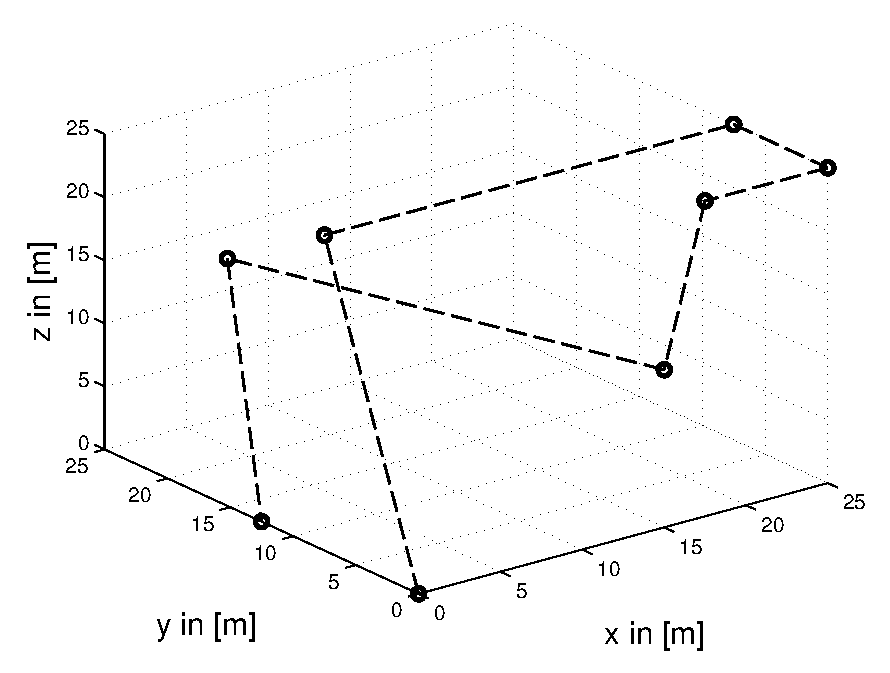
\includegraphics[width = \textwidth]{graphics/sampleNodeAgile}
  \end{minipage}
  \caption{The experimental environment based on three samples. {\bf Left:} The \textit{road} waypoints represent the need of low overshoots to not touch obstacles beside the streets. Its long straight ways enable high velocities. {\bf Center:} The \textit{helix} waypoints represent the circumnavigation of an obstacle with constantly high curvature. {\bf Right:} The \textit{agile} waypoints include both straight sections as well as high curvature.}
  \label{fig:sampleNodes}
\end{figure}

\section{Trajectories and Performance Metrics}
\label{sec:definition}
\subsection{Path vs. Trajectory}
The main difference between a path $ {\bf p}(u)$ and a trajectory $ {\bf \tilde{p}}(t)$ is that only the latter includes time, i.e. considers the dynamics. A path is only defined as the way to go from point a to point b. Therefore it only has geometrical properties. In order to generate a trajectory, a time needs to be assigned to each point on the path. This is done with a function $u=u(t)$ that connects the parameter $u$ of the geometrical path with the time. In the following this function $u=u(t)$ will also be referred to as the motion law as in \cite{snider}. The composition of the $u=u(t)$ and the geometrical path ${\bf p}(u)$ finally forms the trajectory ${\bf \tilde{p}}(t)$. This concept is shown in figure \ref{fig:path_trajectory}.

\begin{figure}[H]
	\centering
    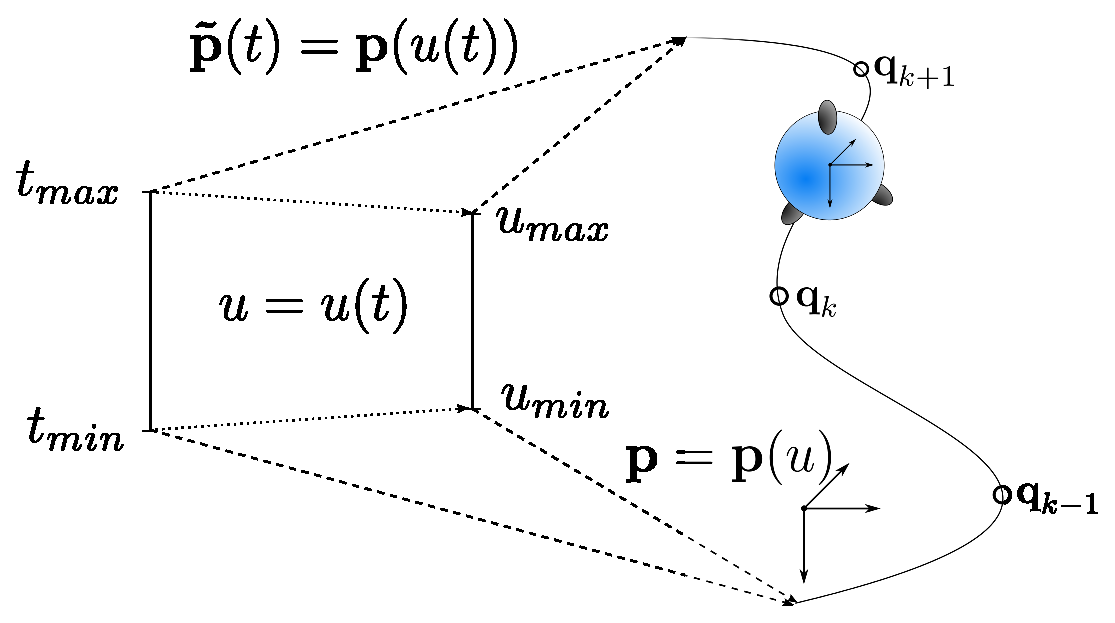
\includegraphics[width = 0.9\textwidth]{graphics/PathTrajectory.eps}
  \caption{Composition of a path ${\bf p}(u)$ and the motion law $u(t)$ forming the trajectory ${\bf \tilde{p}}(t)$}
  \label{fig:path_trajectory}
\end{figure}


In order to get the velocity and acceleration of the trajectory, the chain rule has to be applied to ${\bf \tilde{p}}(t)=({\bf p}\circ u)(t)$:

\begin{align}\label{vel_acc}
{\bf \dot{\tilde{p}}}(t) &= \frac{d {\bf p}}{du}\dot{u}(t) \\
{\bf \ddot{\tilde{p}}}(t) &= \frac{d {\bf p}}{du}\ddot{u}(t)+\frac{d^{2} {\bf p}}{du^{2}}\dot{u}^{2}(t)
\end{align}

%{\bf \ddot{\tilde{p}}}(t)





\subsection{Interpolation vs. Approximation}
If one wants to draw a path through a set of waypoints, we can distinguish between two cases. Firstly, the path can pass through all waypoints no matter how many bends it will have. Secondly, the path tries to best fit the waypoint set, i.e. a function of a  certain order is adopted to best fit the waypoints. This can be done with different methods, e.g with least-squares. The first approach is called interpolation whereas the second approach is called approximation. Depending on the choice, different curves with different properties are formed (see figure \ref{fig:ApproxInterpol}).  


\begin{figure}[H]
	\centering
    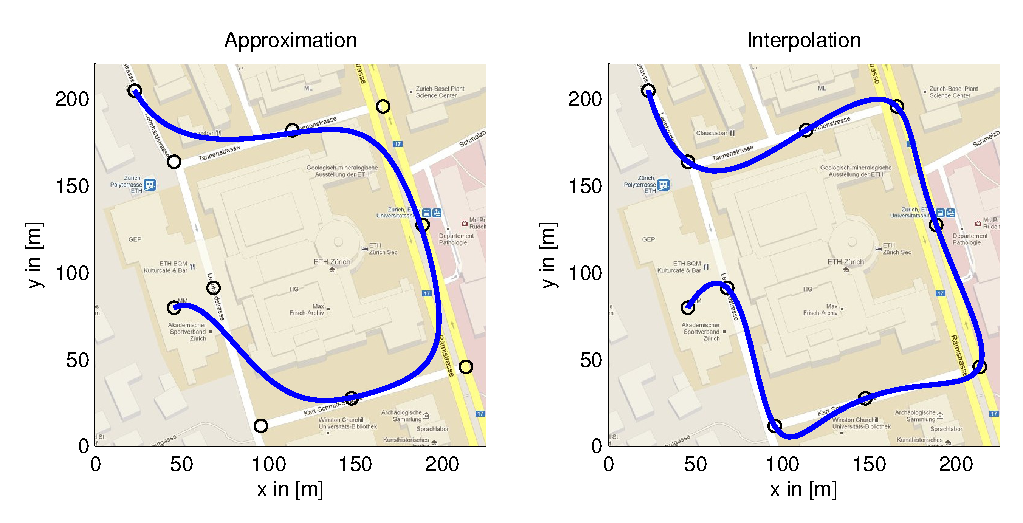
\includegraphics[width = 0.9\textwidth]{graphics/ApproxInterpol.eps}
  \caption{ Waypoints interpolation on the left and waypoints approximation on the right}
  \label{fig:ApproxInterpol}
\end{figure}

For the trajectory planning for \textsc{Skye}, it was necessary to interpolate the waypoints. This is due to the GUI used (see section \ref{sec:realization}). There, only a small amount of waypoints is set and the pilot expects \textsc{Skye} to pass through all of them and not to take any shortcut. I.e.:
\begin{equation}
{\bf p}(u_k)\stackrel{!}{=}{\bf q}_k=\begin{bmatrix}x_k\\y_k\\z_k \end{bmatrix}
\end{equation}

The approximation of the waypoints could result in a collision with buildings as illustrated in \ref{fig:ApproxInterpol}.


To interpolate a given set of $n+1$ waypoints a polynomial (of order $\ge n+1$) from $\varPi_{>n}$ or else a set of polynomials of lower order, defined over a certain interval, can be used. This set of low-order polynomials then forms a spline. As impressively shown in \cite{dahmen}, splines are the best option when interpolating many waypoints, as high order polynomials tend to have high oscillations.

\subsection{Performance Metrics}

To score and optimize the generated trajectories $\tilde{p}(t)$ and the resulting trace of the system $r(t)$ we set up the following performance metrics. The performance metrics (\ref{item:static_deviation}) to (\ref{item:static_acceleration}) are referred to as \textit{static criteria} as they do not depend on any simulation. The remaining ones (\textit{dynamic criteria}) mainly depend on the used controller\footnote{For detailed description of the used notation see section \ref{sec:definition}.}.
\\
Let $L_p$ be the length of the path ${\bf p}(u)$ and $T_p$ the time to cover the trajectory $\tilde{\bf p}(t)$
\begin{equation}
L_p = \int_{u_{min}}^{u_{max}} d{\bf p} \qquad T_p = \int_{t_{min}}^{t_{max}} dt
\label{eq:length_of_path}
\end{equation}
the performance metrics are defined as follows.

\begin{enumerate}[i)] 
\item Average deviation between actual path and chord (straight) connection between waypoints
\label{item:static_deviation}
\begin{equation}
J_1 = \int_{u_{min}}^{u_{max}} \|{\bf p}(u)- {\bf p}_2(u)\| du \cdot L_p^{-1} \label{eq:static_deviation}
\end{equation}

\item Average curvature of the path\footnote{For a derivation of curvature see any vetor analysis book, e.g. \cite{stammbach} chapter II, page 71.}
\label{item:static_curvature}
\begin{equation}
J_2 = \int_{u_{min}}^{u_{max}} \frac{\| \frac{d {\bf p}}{du} \times \frac{d^{2} {\bf p}}{du^{2}} \|}{\|  \frac{d {\bf p}}{du} \|^3}du \cdot L_p^{-1}
\label{eq:static_curvature}
\end{equation}
% THIS ALTERNATIVE NOTATION IS INCONSEQUENCE IN USING DOT WHEN NOT HAVING PARAM T !!
% J_2 = \int_{u_{min}}^{u_{max}} \frac{\| \dot{\bf p}(u) \times \ddot{\bf p}(u) \|}{\| \dot{\bf p}(u) \|^3}du \cdot L_p^{-1}

\item Average acceleration of the trajectory
\label{item:static_acceleration}
\begin{equation}
J_3 = \int_{t_{min}}^{t_{max}} \|{\bf \ddot{\tilde{p}}}(t)\| dt \cdot T_p^{-1} \label{eq:static_acceleration}
\end{equation}

\item Deviation between trajectory and trace of the system\footnote{The deviation vector between trace and its closest point on the trajectory is always normal to the latter. Compare with figure \ref{fig:scene_crossTrack}.}
\label{item:dynamic_deviation}
\begin{equation}
J_4 = \int_{t_{min}}^{t_{max}} \| {\bf \tilde{p}}(t_{cl}) - {\bf r}(t) \| dt \cdot T_p^{-1} 
\label{eq:dynamic_deviation}
\end{equation}

\item Average acceleration of the system
\label{item:dynamic_acceleration}
\begin{equation}
J_5 = \int_{t_{min}}^{t_{max}} \|{\bf \ddot{r}}(t)\| dt \cdot T_p^{-1}
\end{equation}

\item Temporal synchrony\footnote{Temporal should be warranted for accurate \textit{trajectory} following. In \textsc{Skye}'s task of caputuring time independent imagery, it was only considered as a secondary aspect.}
\label{item:dynamic_synchrony}
\begin{equation}
J_6 = \| {\bf \tilde{p}}(t_{max}) - {\bf r}(t_{max}) \| \cdot L_p^{-1} \label{eq:dynamic_synchrony}
\end{equation}

\end{enumerate}





\section{Splines}
\label{sec:splines}
\subsection{Parameterization}
\label{subsec:parameterization}
A so called knot vector ${\bf u}$ composed of a nondecreasing sequence of $u_0 < u_1 < ...< u_n$ must be found in order to calculate a spline for each dimension going through the $n+1$ waypoints.

\begin{equation}
%{\bf x}(u) =  \begin{bmatrix} p_x(u) \\ p_y(u) \\p_z(u) \end{bmatrix}
{\bf p}(u) =  \begin{bmatrix} p_x(u) \\ p_y(u) \\p_z(u) \end{bmatrix}
\end{equation}


In this section, the most common used techniques are analyzed\footnote{A vaster evaluation of different parameterizations can be found in \cite{haron}}. The choice of parameterization affects the geometrical properties of the path on the one hand and the velocity and acceleration of the trajectory on the other hand (see equation \eqref{vel_acc}). The latter is especially of big impact if a proportional relation is used to describe the motion law, i.e. $u=\lambda t$ (see section \ref{sec:motionLaw}).

\subsubsection{Uniform}
This is the simplest way to define the knot vector $\bf u$. Here, the index number of the waypoints is assigned to $u$.
\begin{equation*}
u_k-u_{k-1}= 1
\end{equation*}
\subsubsection{Chord Length}
In this method the chord length (the blue line in figure \ref{fig:arcLength} between the waypoints is calculated and then summed up and assigned to $u$. With $u=\lambda t$ this method can be interpreted to aim for a more or less constant velocity over the whole trajectory.
\begin{equation*}
u_k-u_{k-1}=\left \| \begin{bmatrix}x_k\\y_k\\z_k \end{bmatrix}-\begin{bmatrix}x_{k-1}\\y_{k-1}\\z_{k-1} \end{bmatrix}\right \|
\end{equation*}
\subsubsection{Arc Length}
The arc length method is an improved version of the chord length distribution in order to reach a constant velocity. Here instead of taking the chord length between two waypoints, the arc length is estimated using arcs $B_a$ and $B_b$ (see the green arcs in figure \ref{fig:arcLength}) and summed up. %The algorithm\footnote{The algorithm was taken from \cite{engeln} and implemented in \textsc{Matlab}.} for that can be found in \ref{subsec:arcLengthDistribution}.

\begin{equation*}
u_k-u_{k-1}=\frac{B_a+B_b}{2}
\end{equation*}

\begin{figure}[H]
	\centering
    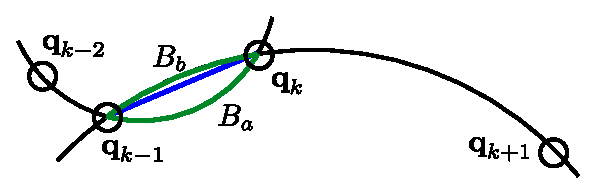
\includegraphics[width = 0.9\textwidth]{graphics/arcLength.eps}
  \caption{The arc length is estimated using the segments, $B_a$ and $B_b$ of two circles where as the chord length is the straight connection.}
  \label{fig:arcLength}
\end{figure}




\subsubsection{Centripetal}
This method was proposed in \cite{lee}. Here the root of the chord length is used. The motivation for this method is, that the larger the angular change from $\textnormal{waypoint}_{n-1}$ to $\textnormal{waypoint}_n$, the more centripetal force is accepted. A justification for this statement can be found in \cite{doessegger} and \cite{lee}.
\begin{equation*}
u_k-u_{k-1}=\sqrt{\left \| \begin{bmatrix}x_k\\y_k\\z_k \end{bmatrix}-\begin{bmatrix}x_{k-1}\\y_{k-1}\\z_{k-1} \end{bmatrix}\right \|}
\end{equation*}

\subsubsection{Discussion}

%geometrical properties, dynamical properties, Kreb'sche Bewertungsalgrithmen:) \textbf{pictures of all of them, justify choice, say that if more waypoints, different decision}

All those four methods were tested on our three sample waypoints defined in \ref{sec:experimental design}. Since the helix waypoints all have the same distance between each other, all four methods result in the same path, respectively trajectory. As the chord and arc length distribution try to maintain a constant velocity, high curvature will be omitted. This however leads to overshoots as seen in figure \ref{fig:parameterizations4_road_agile}. Choosing cubic splines reduces this effect whereas quintic splines amplify it (compare figure \ref{fig:parameterization_cqq}).

\begin{figure}[H]
	\centering
    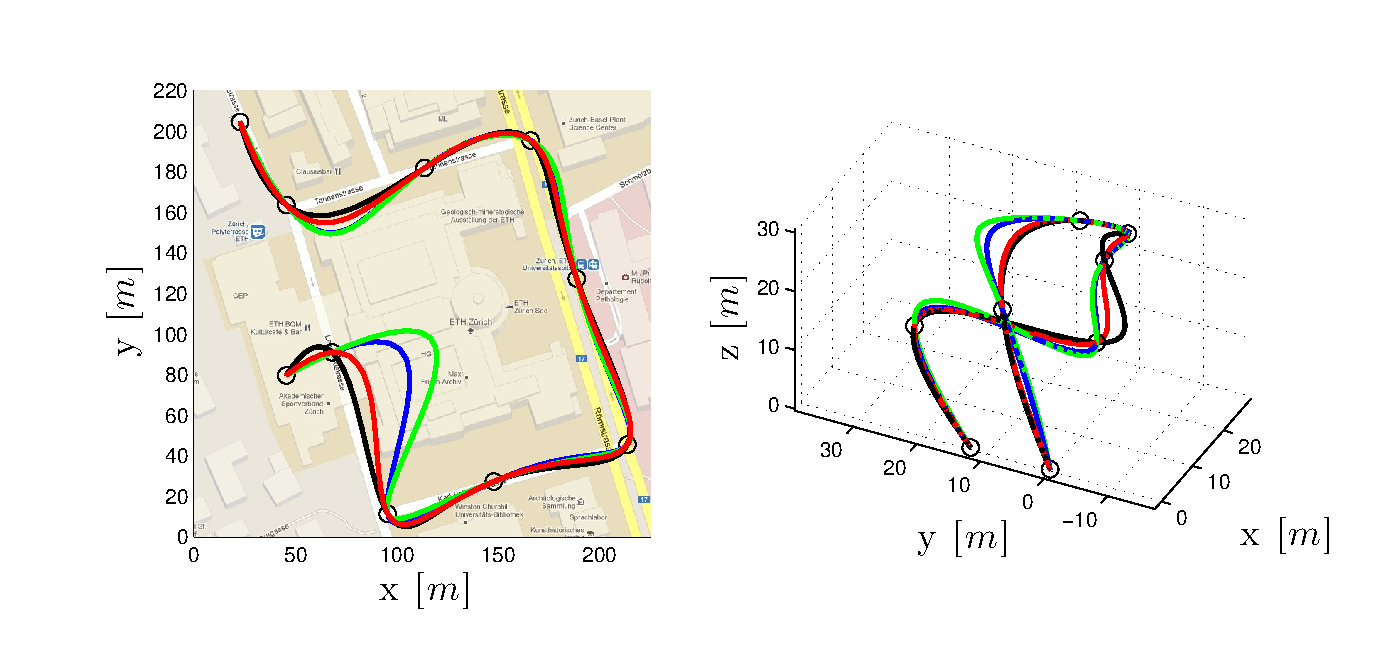
\includegraphics[width = 0.9\textwidth]{graphics/Parameterizations4_road_agile.eps}
  \caption{The different parameterizations shown with quartic splines: Uniform (black), chord length (blue), arc length (green), centripetal (red).}
  \label{fig:parameterizations4_road_agile}
\end{figure}

Since those overshoots are intolerable, a uniform or centripetal distribution has to be chosen. Although in our sample waypoints the two variants seem to be quite similar, the uniform distribution sometimes leads to  loops or cusps as shown in \cite{lee} and \cite{haron}. This occurs, if the chord distance between the waypoints suddenly changes a lot as the uniform distribution is completely independent of the waypoint set. Therefore the centripetal distribution was chosen to best fit our needs.
\\
Beside the geometrical appearance due to the different distributions, the dynamic properties\footnote{In \cite{mellinger} e.g. they optimize the $u$ values to obtain the time optimal trajectory.} are also of big interest, especially if a constant time scaling is used as described in section \ref{subsec:motionLaw}.
Here, as the centripetal distribution is already chosen due to its geometrical properties, this is only shown for reasons of completeness.
However, if the waypoints were set in a closer succession, the geometrical properties would not be that important anymore and the decision should be rethought.

\begin{figure}[H]
	\centering
    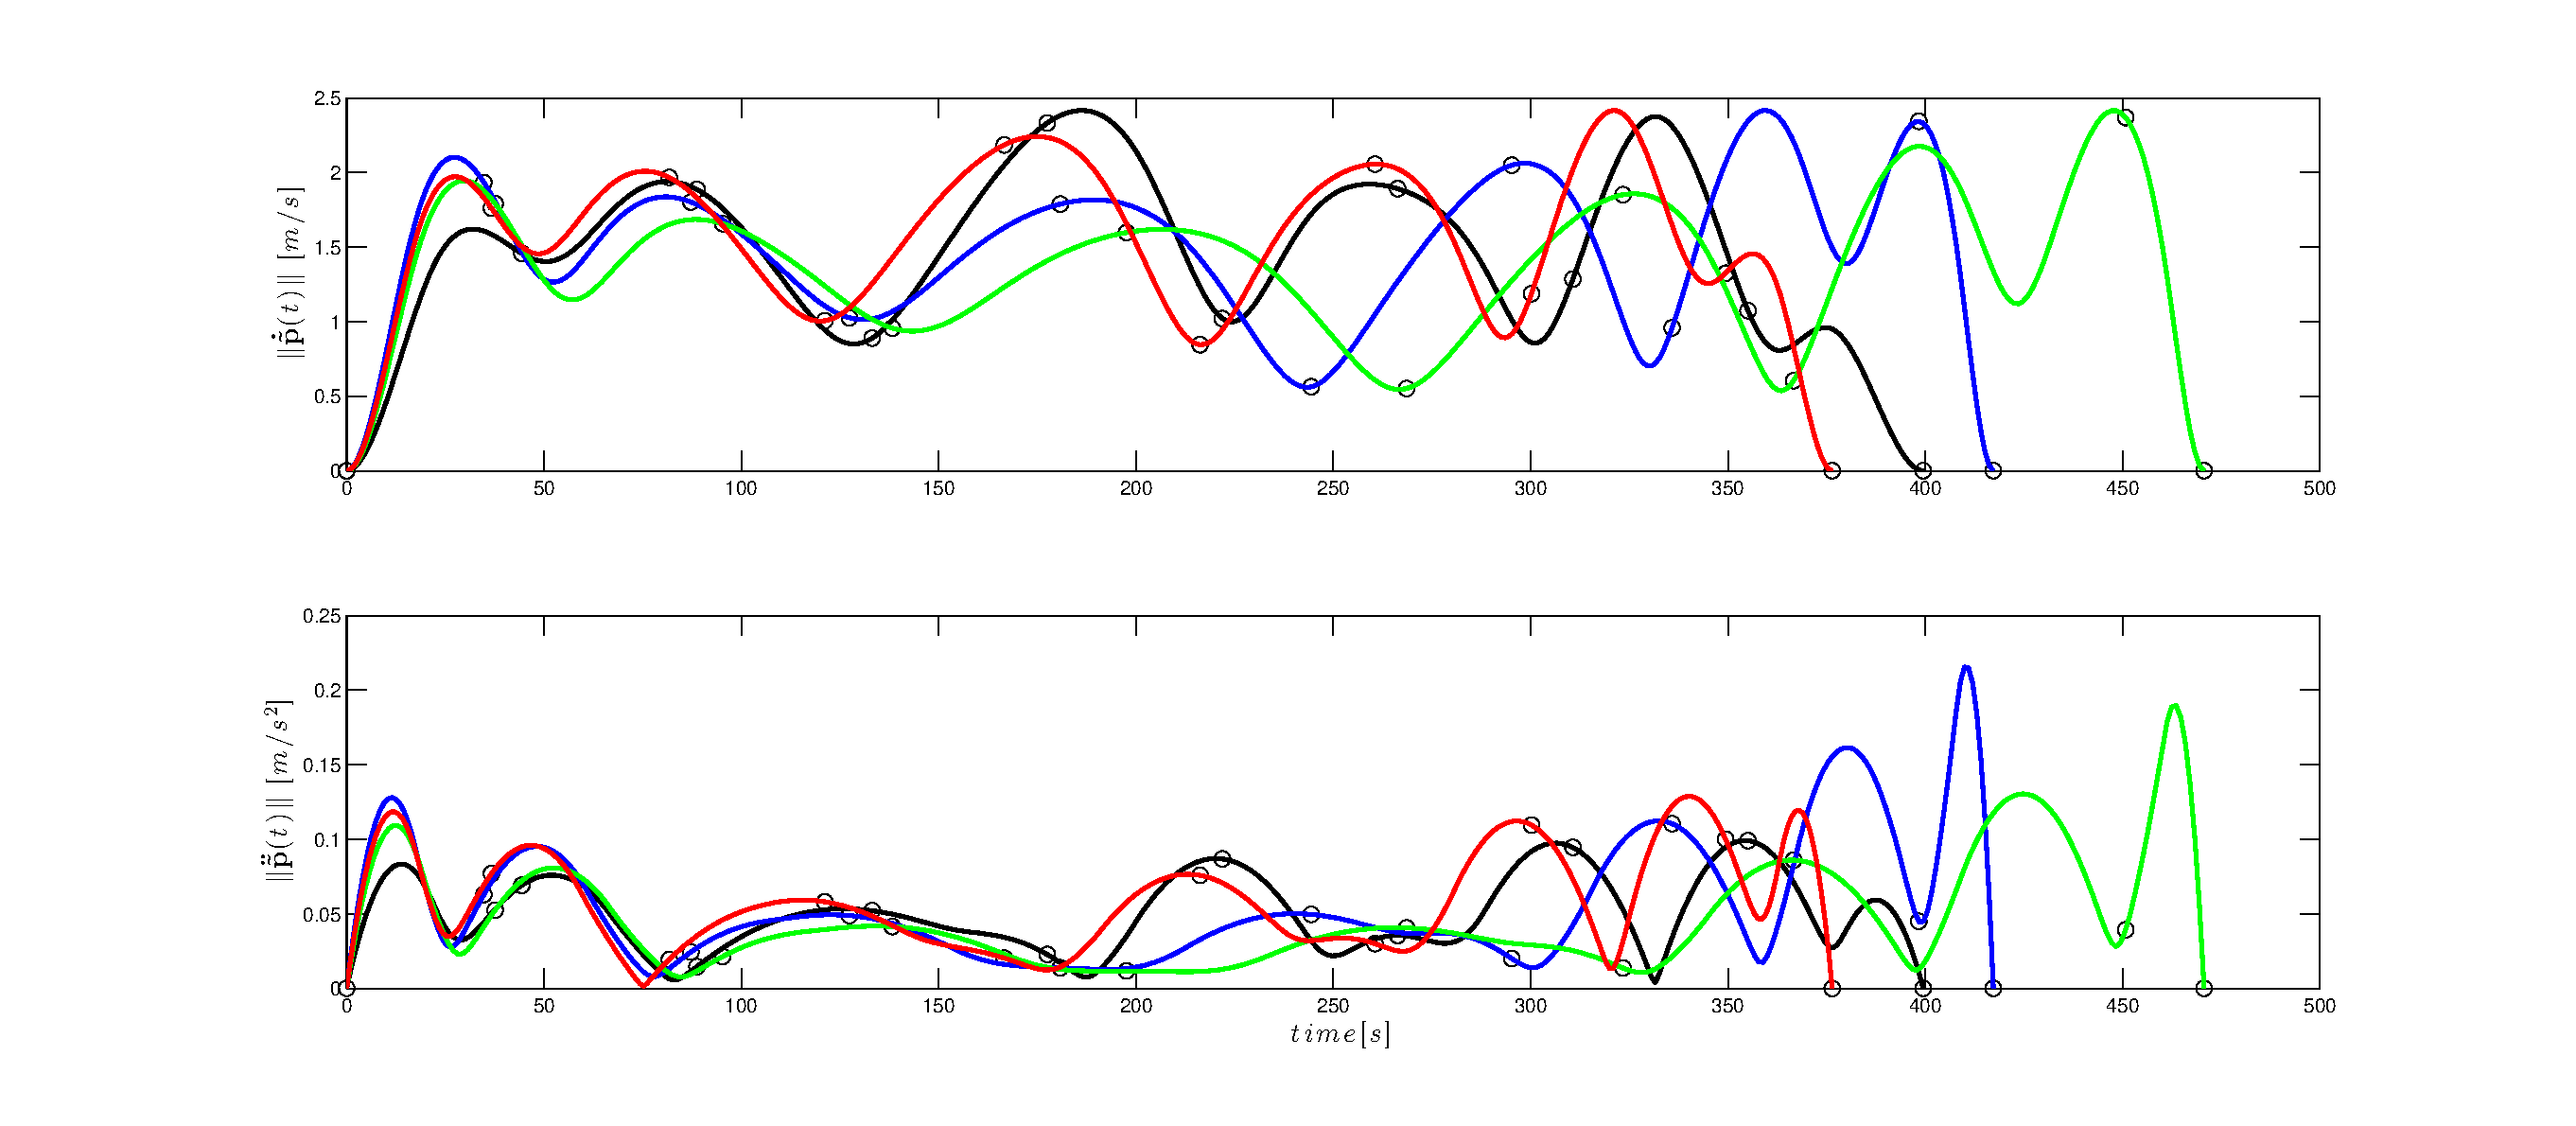
\includegraphics[width = \textwidth]{graphics/Parameterization4_road_vel_acc.eps}
  \caption{Velocity and acceleration of the \textit{road} trajectory generated with quartic splines. In this case the motion law limits the maximum velocity whereas the acceleration remains below its limit. Parametrizations: Uniform (black), chord length (blue), arc length (green) and centripetal (red).}
  \label{fig:para road vel acc}
\end{figure}

In figure \ref{fig:para road vel acc} or table \ref{tab:results_parameterization_road_quartic} respectively, the effect of the different distributions on the velocity and acceleration resulting from a constant time scaling can clearly be seen with quartic splines. The chord length as well as the arc length distribution keep the velocity more or less constant but start oscillating at the end of the track. For cubic splines the situation is slightly different(see appendix \ref{cha:appendix} for a complete overview), but over all criteria centripetal yields the best result.


\begin{table}[H]
\begin{center}
 \begin{tabular}{lll|rrrr}
 \hline
 Cubic \textit{Road} & & Unit & Uniform & Chord Length & Arc Length & Centripetal \\ \hline \hline
 Av. Deviation  & $J_1$ & $[\si{\meter}]$    & 4.043 & 8.452 & 10.963 & 4.774 \\
 Av. Curvature & $J_2$ & $[\si{\per\meter}]$ & 0.050 & 0.036 & 0.032 & 0.047 \\
 Av. Acceleration  & $J_3$ & $[\si{\meter\per\square\second}]$ &  0.062 & 0.449 & 0.506 & 0.139 \\
 Time      &   & $[\si{\second}]$ &  399.5 & 417.3 & 470.6 & 376.4 \\
 \hline
 \end{tabular}
 \caption{Comparison of the parameterizations. Static criteria are listed for quartic trajectories using the \textit{road} waypoints.}\vspace{1ex}
 \label{tab:results_parameterization_road_quartic}
\end{center}
\end{table}

\subsection{Spline Degree}

\subsubsection{Continuity}
When selecting a spline, the spline's order shall also be chosen, i.e. of what degree are the polynomials which make up the spline curve. If polynomials of degree one are used, the first derivative of the curve will not be continuous anymore. We say that this curve has a geometrical continuity of $G^0$. In the case of a trajectory, the geometrical continuity of the path will directly have an influence on the continuity of the motion as can be seen from the equations \eqref{vel_acc} or in figure \ref{fig:continuity}. E. g. with a motion law of $u=\lambda t$, cubic splines are discontinuous in the jerk, whereas quartic are still continuous and quintic splines would be continuous up to the snap, i.e. ${\bf \tilde{p}}(t)$ would have a parametric continuity of $C^4$ . 

\begin{figure}[H]
	\centering
    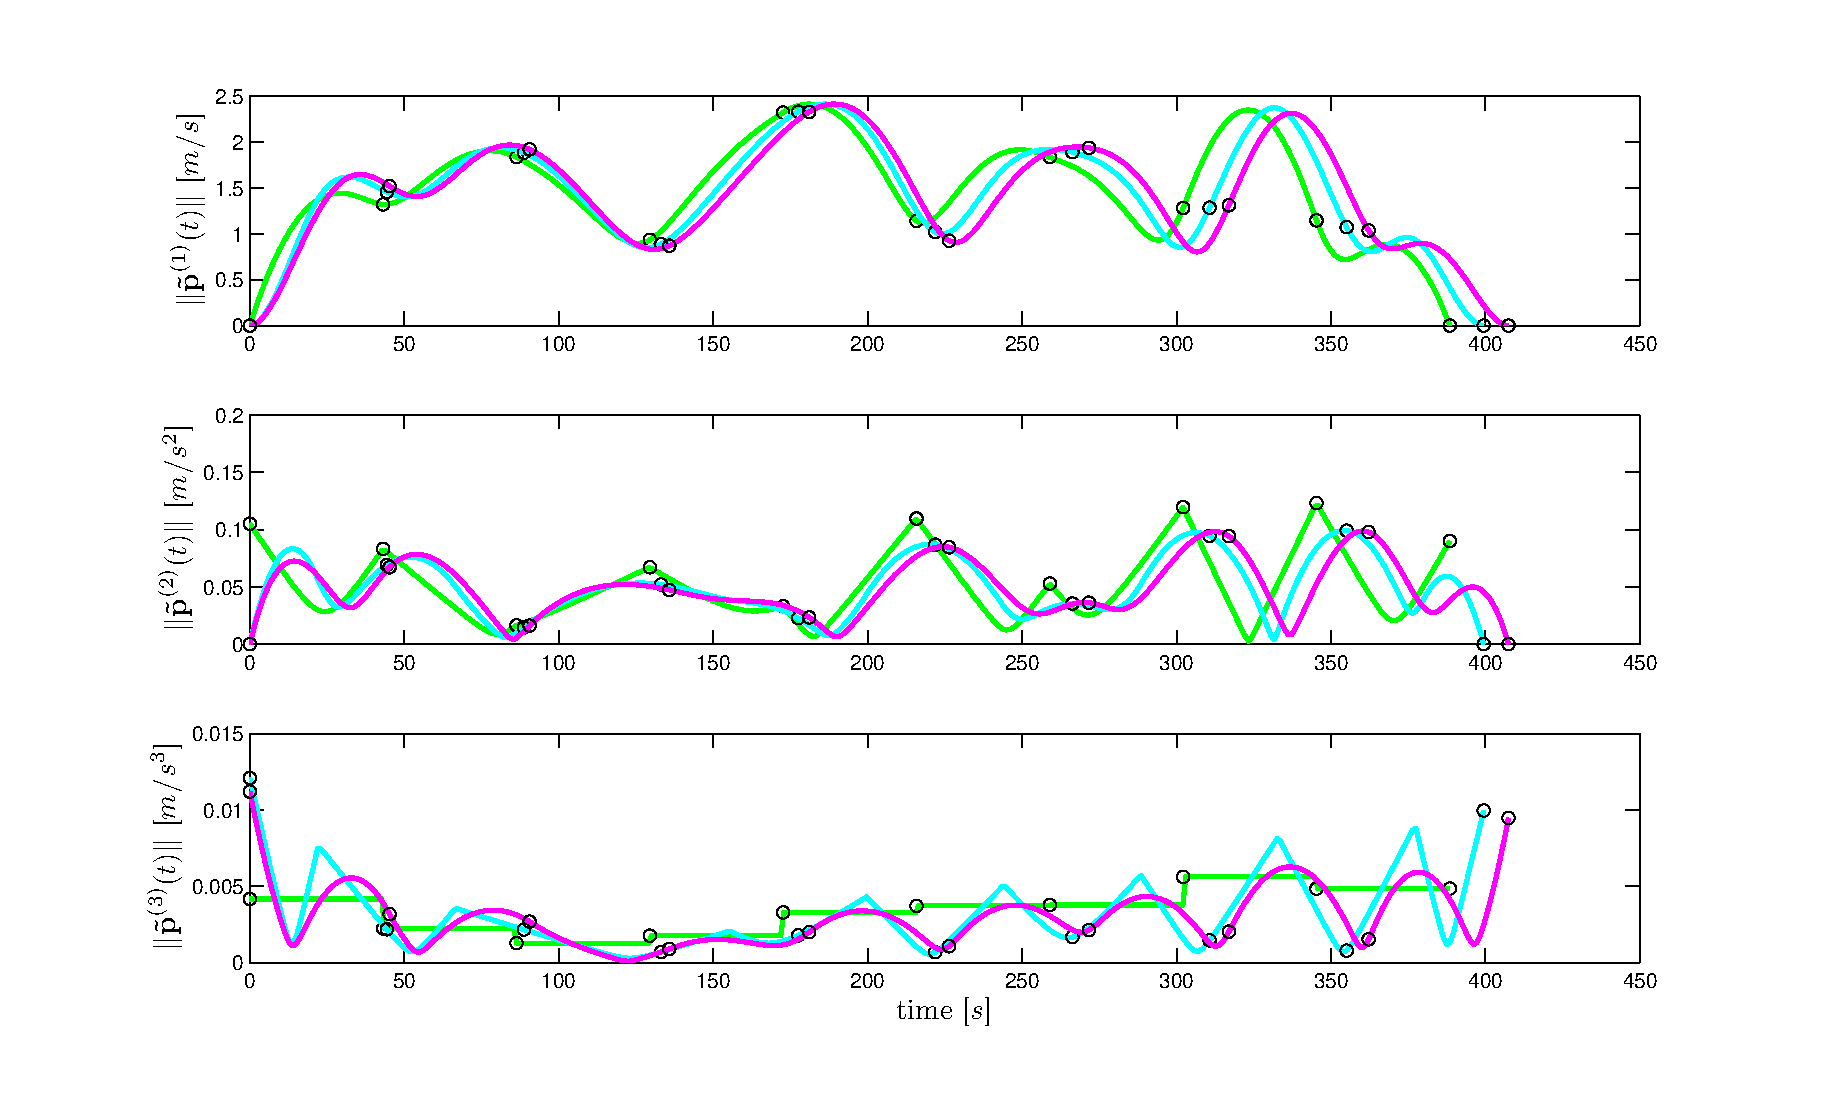
\includegraphics[width = \textwidth]{graphics/continuity.eps}
  \caption{The different degrees of continuity for cubic (green), quartic (cyan) and quintic (magenta) splines.}
  \label{fig:continuity}
\end{figure}

For \textsc{Skye} it was intuitively clear that at least cubic splines had to be used, i.e. a parametric continuity of $C^2$ was needed (continuity in acceleration). This is due to its propulsion system, which is briefly described in section \ref{sec:system overview} and in detail in \cite{schaffnervu}. The orientation of the thrusters cannot be changed immediately, i.e. the positioning motor needs time to turn the thruster to the requested direction. Therefore the trajectory should not ask for a step input for the orientation of the thrusters, which is respected by using cubic splines or splines of higher degree (see figure \ref{fig:qc_rpm}). However, in order to find out whether even the dynamics of the thrusters or further dynamics of the positioning motor have to be considered, the whole propulsion system was fed with forces calculated from the accelerations $F_x=m_{tot}a_x$. As it can be seen from figure \ref{fig:forces}, the propulsion system is able to handle all the resulting inputs of cubic, quartic and quintic splines.
 
\begin{figure}[H]
	\centering
    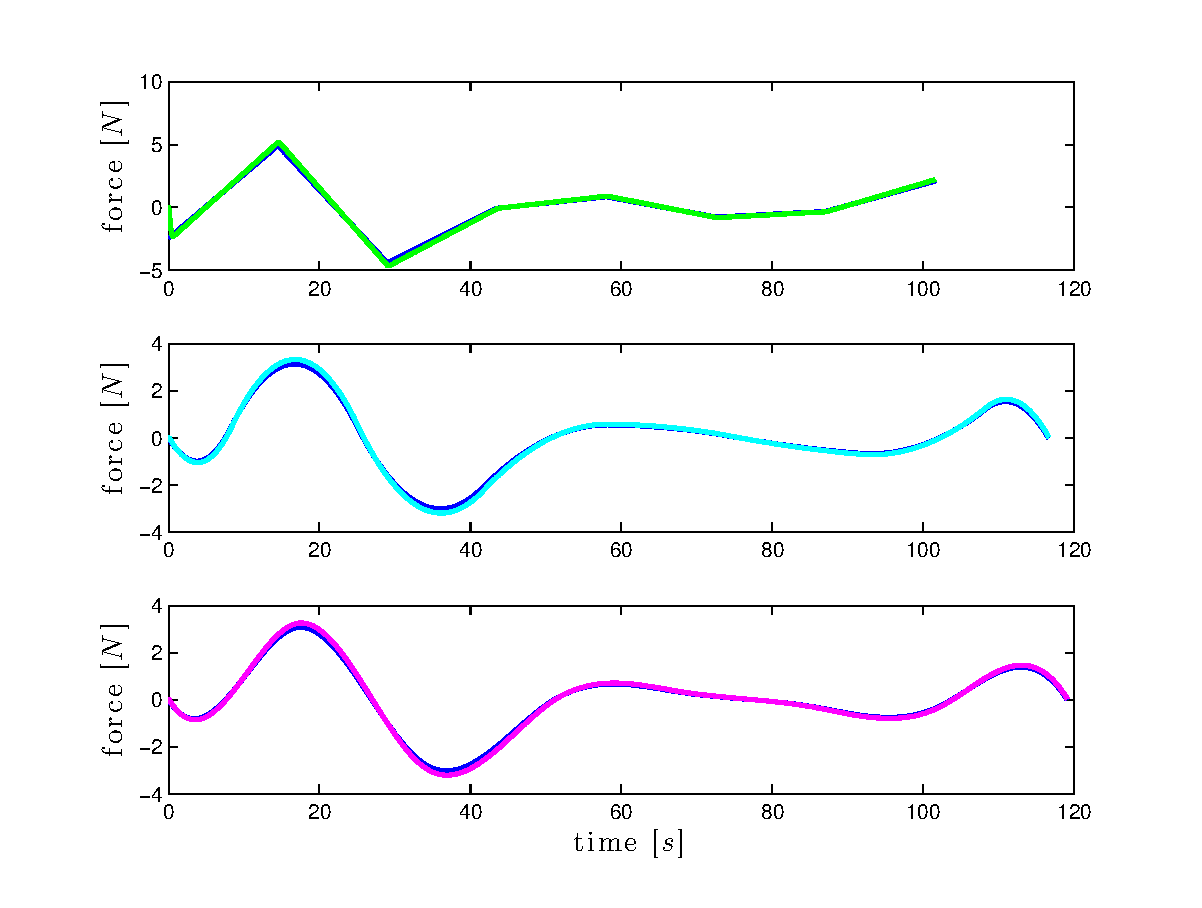
\includegraphics[width = \textwidth]{graphics/forces.eps}
  \caption{The comparison of the forces output of the propulsion system with the forces input resulting from the different degrees of splines; input (blue), output: cubic (green), quartic (cyan) and quintic (magenta) for the \textit{agile} waypoints.}
\label{fig:forces}
\end{figure} 

%The small deviations between the input and the output forces are a result of interpolation, done in the propulsion system \cite{schaffnervu}, and are not a result of an inadequate input. However, BLABLA.....see deviations, but much faster dynamics therefore neglectable.
%{\bf here static criteria?}

\subsubsection{Geometrical Appearance}
Beside the continuity and the dynamic properties again the geometrical appearance needs to be considered in order to choose the best degree of splines for \textsc{Skye}. As shown in figure \ref{fig:degreeCentripetal}, the cubic splines are most suitable to use with a not so dense set of waypoints. Quartic and qubic splines have higher overshoots, which would need to be omitted by setting waypoints more densely. As this would be cumbersome with the GUI described in chapter \ref{cha:findHardSoftSolution}, cubic splines are most suitable. 

\begin{figure}[H]
	\centering
    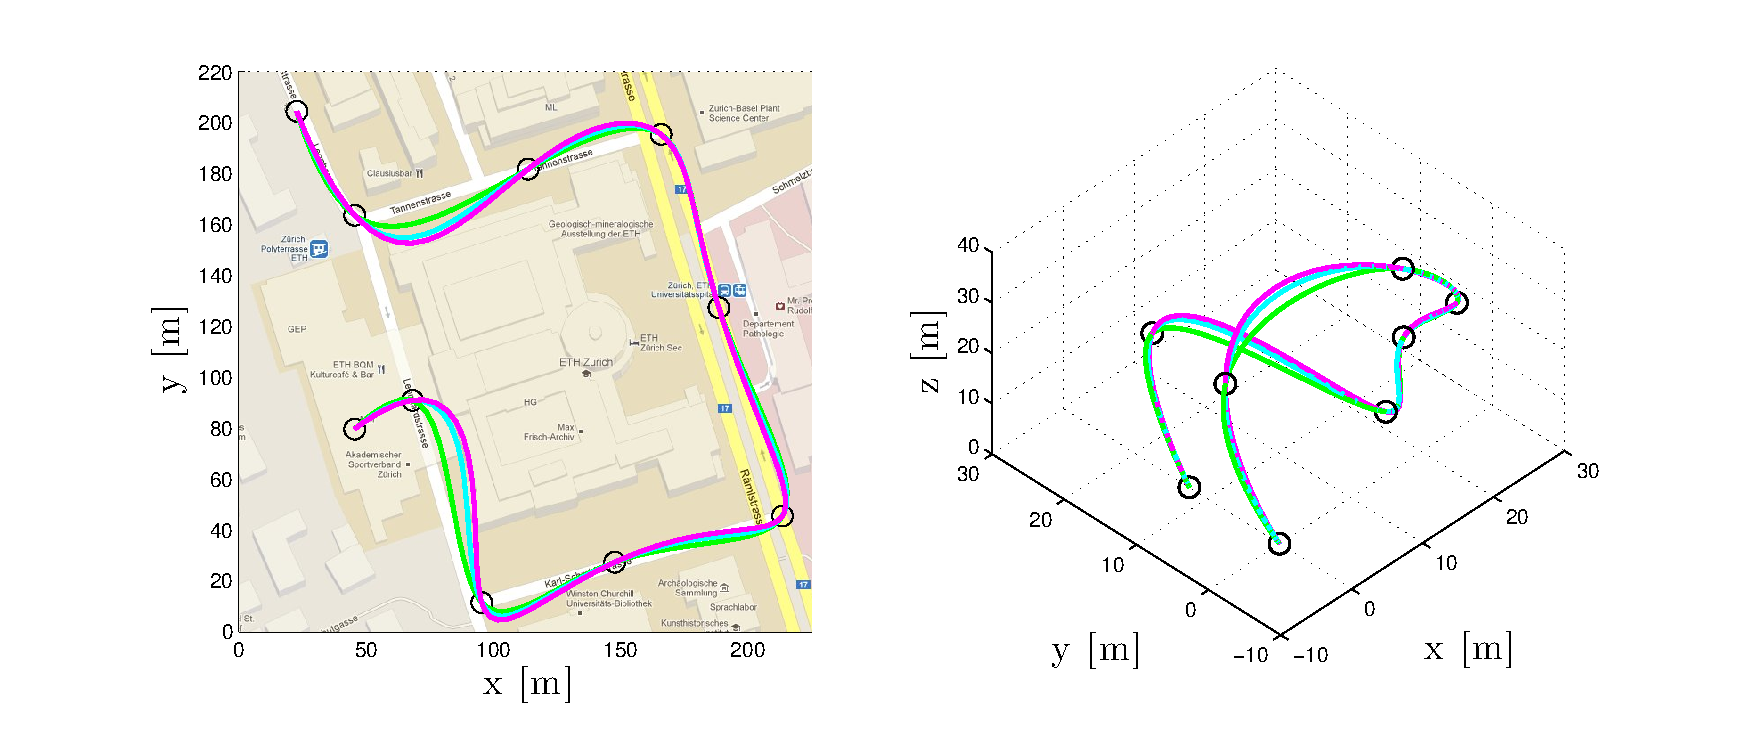
\includegraphics[width = \textwidth]{graphics/DegreeCentripetal_road_agile.eps}
  \caption{The comparison of the cubic (green), quartic (cyan) and quintic (magenta) splines with a centripetal parameterization of the waypoints}
  \label{fig:degreeCentripetal}
\end{figure} 






\subsection{Boundary Conditions}
\label{subsec:boundary conditions}

If $p_x(u)$ is a spline of degree $p$ and consists of $n_{knots+1}$ knots\footnote{Knots are the places where the polynomial pieces are connected.}, it has $p+n_{knots}$ degrees of freedom. The polynomial of the first interval $a_0^p(u)$ has $p+1$ degrees of freedom. The polynomial for the second interval $a_1^p(u)$ is given by
\begin{equation*}
a_0^{p(j)}(u_1)=a_1^{p(j)}(u_1),~j=0,...,p-1
\end{equation*}
Therefore $a_1^p(u)$ will only provide one additional degree of freedom. This is also true for all the following intervals. The spline $p_x(u)$ has finally $p+n_{knots}$ degrees of freedom\footnote{For a more mathematical proof refer to \cite{dahmen}.}. Using piecewise polynomials the number of the waypoints $n+1$ is also the number of knots $n_{knots}+1$. Given the parameter $u$ for all the $n+1$ waypoints yields $p+n_{knots}-(n_{knots}+1) = p-1$ constraints that still have to be imposed. As a constant time scaling is used\footnote{ See section \ref{subsec:motionLaw}. Also a non linear solution is described.} it is necessary to define:

\begin{equation*}
\frac{dp_x(u)}{du} \Bigm|_{u=u_0} = \frac{dp_x(u)}{du} \Bigm|_{u=u_n}=0
\end{equation*}

in order to have the velocity at the start and at the end of the trajectory to equal zero

\begin{equation*}
\dot{\tilde{p}}_x(t_{start}) = \dot{\tilde{p}}_x(t_{end})=0
\end{equation*}

For quintic splines two additional constraints can be set

\begin{equation*}
\frac{d^2p_x(u)}{du^2} \Bigm|_{u=u_0} = \frac{d^2p_x(u)}{du^2} \Bigm|_{u=u_n}=0
\end{equation*}

such that also the acceleration at the start and at the end of the trajectory is zero (compare with equation \eqref{vel_acc}). For quartic splines also two additional constraints can be set if B-splines are used and the knots are shifted as described in section \ref{subsec:implementation}. \\
These boundary conditions are set for all dimensions.



\subsection{Implementation}
\label{subsec:implementation}
As the implementation of the spline generation was not the goal of this bachelor thesis, it was decided to use \textsc{Matlab}'s Curve Fitting Toolbox.
Yet it soon became evident that in order to correctly set boundary conditions for quartic and quintic splines and to get a thorough understanding, it was best to program the algorithms and only use the toolbox to make calculations with the generated splines.\\

\subsubsection{Spline Basis}
The common known basis for a spline $p_x(u)$ of degree $p$ is the piecewise polynomial\footnote{A spline made of these piecewise polynomials is in \textsc{Matlab} named to be of pp-form.} basis.
For each knot span $[u_j, u_{k+j})$ a polynomial $a_j^p$ of degree $p$ is defined. 
\begin{equation}
p_x(u)=a_j^p(u),~u \in [u_j,u_{j+1})
\end{equation}
Using piecewise polynomials, the number of waypoints $n+1$ equals the number of knots $n_{knots+1}$.


\paragraph{Ex. 1:}
Given a data set of four waypoints, i.e. $n+1=4$, with values of the x-coordinate of ${\bf x} = [1,2,3,3]$ and a knot vector of ${\bf u}=[0,2,3,5]$ received through one of the methods described in section \ref{subsec:parameterization}. For a interpolation with a linear spline, $p=1$, three polynomial pieces $a_j^1(u)=d_j+e_j,~j=0,1,2$ need to be found, such that continuity is granted. For this example their coefficients are found to be: ${\bf d}=[\frac{1}{2},1,0]$ and ${\bf e}=[1,0,3]$. The resulting spline is shown in figure \ref{fig:ppSpline}.

\begin{figure}[H]
	\centering
    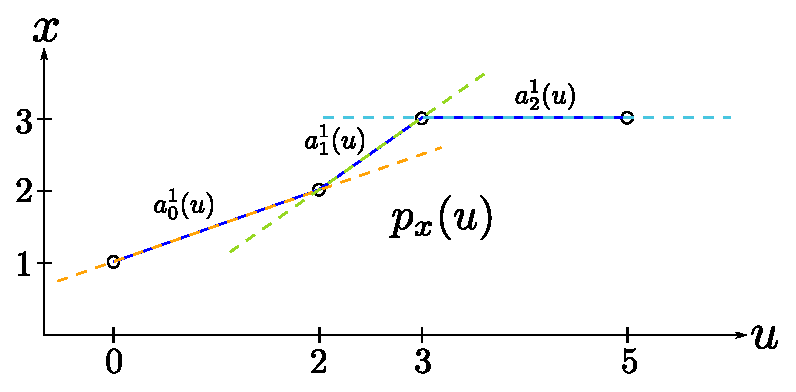
\includegraphics[width = 0.8\textwidth]{graphics/ppSpline.eps}
  \caption{Visualization of the common used piecewise polynomial basis to form the linearly interpolating spline of example Ex. 1}
  \label{fig:ppSpline}
\end{figure} 


Another often used basis for a spline is the one of the basic splines (B-splines\footnote{A spline made of these B-splines is in \textsc{Matlab} named to be of B-form.}). Instead of defining a polynomial of degree $p$ for each knot span, a linear combination of B-splines $B_j^p(u)$ of degree $p$ is taken to form $p_x(u)$.
\begin{equation}
p_x(u) = \sum_{j=0}^m {c_x}_jB_j^p(u), ~u_{min} \leq u \leq u_{max}
\end{equation}

Whereas these B-splines are defined recursively using the Cox-de Boor recursion formula:
 
 \begin{align}
B_j^0(u) &= \begin{cases} 1,&\text{if}~ u_j \leq u < u_{j+1}\\
					0,&\text{otherwise}
		\end{cases}\\
B_j^p(u) &= \frac{u-u_j}{u_{j+p}-u_j}B_j^{p-1}(u)+\frac{u_{j+p+1}-u}{u_{j+p+1}-u_{j+1}}B_{j+1}^{p-1}(u), ~p>0
\end{align}

The shapes of the first three degrees of B-splines with a not equally distributed knots are shown in figure \ref{fig:BSplines_definition}.

\begin{figure}[H]
	\centering
    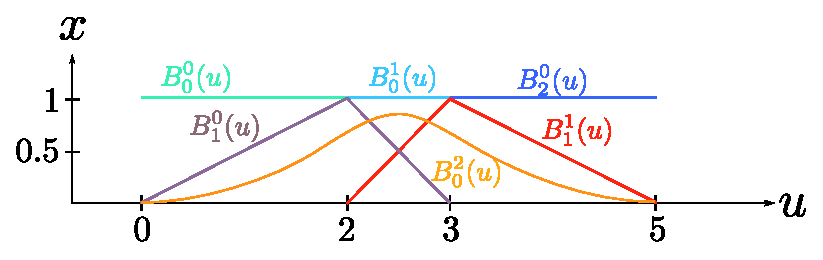
\includegraphics[width = 0.8\textwidth]{graphics/BSplineBasis.eps}
  \caption{B-splines bases up to degree $p=2$. The number of bases is reduced by increasing its order. The knot vector $u=[0,2,3,5]$ is the same as used in Ex. 1.}
  \label{fig:BSplines_definition}
\end{figure} 

With this definition of B-splines, the number $m+1$ of resulting B-splines is given by:
 
\begin{equation}
\label{n_knot-m-p-relation}
m+1=n_{knot}-p
\end{equation} 

If $n+1=n_{knot}+1$ still held true, only $m+1=n-p$ B-splines would result. They would not represent a basis to interpolate the $n+1$ waypoints with a spline of degree $p$. For intuition figure \ref{fig:BSpline} of example  Ex. 2 might help. There the same waypoints set as in figure \ref{fig:ppSpline} is used. Not extending the knot vector would result in only two B-splines of degree 1 ($B_1^1$ and $B_2^1$ in the visualization) as equation \eqref{n_knot-m-p-relation} would result in $m=1$. These two B-Splines would not form a basis to linearly interpolate all four waypoints. \\
In order to have a basis to interpolate $n+1$ waypoints with a spline of degree $p$, it is proposed in \cite{biagiotti} to extend the knot vector ${\bf u}$ in the following way:\\
\\
If the degree $p$ of the interpolating spline is odd:
\begin{equation}
{\bf u}_{extended}= \underbrace{ [u_0,\ldots,u_0}_{p+1},u_1, \ldots,u_{n-1},\underbrace{u_n,\ldots, u_n ]}_{p+1} 
\end{equation}
If the degree $p$ of the interpolating spline is even:
\begin{equation}
{\bf u}_{extended}= \underbrace{ [u_0,\ldots,u_0}_{p+1},(u_0+u_1)/2, \ldots, (u_{k-1}-u_k)/2, \ldots,(u_{n-1}+u_n)/2,\underbrace{u_n,\ldots, u_n ]}_{p+1} 
\end{equation} 
Latter shifting of the knots is used to reduce the oscillations that splines of even degree usually have\footnote{These oscillations can be seen in \cite{doessegger} as there no shifting is used.} and also enables to set symmetric boundary conditions as described in section \ref{subsec:boundary conditions}. The extended knots vector with the resulting B-splines finally will form a basis. For a prove \cite{dahmen} is recommended.

\paragraph{Ex. 2:}
Given the same waypoints as in example Ex. 1, ${\bf u}_{extended}$ is defined to be $[0,0,2,3,5,5]$. Over this knot vector the B-splines can be determined and and the coefficients\footnote{These coefficients are also said to span a control polygon.} ${c_x}_j$ are calculated to be ${\bf c}_x=[1,2,3,3]$ using equation \eqref{eq:linearSysofEq}.

\begin{figure}[H]
	\centering
    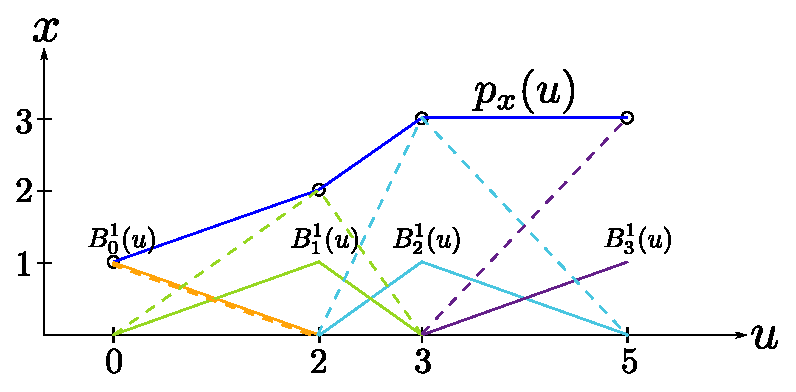
\includegraphics[width = 0.8\textwidth]{graphics/BSpline.eps}
  \caption{Visualization of B-splines forming a basis for the linearly interpolating spline of Ex. 2}
  \label{fig:BSpline}
\end{figure} 

\subsubsection{Realization}
While for cubic splines the piecewise polynomial approach from \cite{engeln} was chosen, B-splines were taken as a basis for the quartic and quintic splines and the proposed C-Code in \cite{biagiotti} was implemented in \textsc{Matlab} to get the B-splines.\\
\\

Once the extended knot vector ${\bf u}_{extended}$ is defined and the boundary conditions are set, the only thing left is to solve the following linear system of equations for all dimensions in order to get the coefficients ${\bf c}_j$,  here shown for $x$:
\begin{equation}
\label{eq:linearSysofEq}
{\bf A}_{[m+1\times m+1] }{{\bf c}_x}_{[m+1\times 1]}={{\bf b}_x}_{[m+1 \times 1]}
\end{equation}
where


\begin{equation*}
    {\bf c}_x = [ {c_x}_{0}, {c_x}_{1}, \ldots, {c_x}_{m-1}, {c_x}_{m}]
\end{equation*}

and

\begin{equation*}
{\bf A}=   \begin{bmatrix} % or pmatrix or bmatrix or Bmatrix or ...
      B_0^p(u_0)        & B_1^p(u_0)         & \ldots & B_m^p(u_0) \\
      B_0^{p(1)}(u_0) & B_1^{p(1)}(u_0) & \ldots & B_m^{p(1)}(u_0) \\
      B_0^{p(2)}(u_0) & B_1^{p(2)}(u_0) & \ldots & B_m^{p(2)}(u_0) \\
      B_0^p(u_1)         & B_1^p(u_1)         & \ldots & B_m^p(u_1) \\
      \vdots			&\vdots		     &            &\vdots \\
      B_0^p(u_{n-1})        & B_1^p(u_{n-1})         & \ldots & B_m^p(u_{n-1}) \\
      B_0^{p(2)}(u_n) & B_1^{p(2)}(u_n) & \ldots & B_m^{p(2)}(u_n) \\
      B_0^{p(1)}(u_n) & B_1^{p(1)}(u_n) & \ldots & B_m^{p(1)}(u_n) \\
      B_0^p(u_n)         & B_1^p(u_n)         & \ldots & B_m^p(u_n) \\
      
   \end{bmatrix},
   \quad 
   {\bf c_x} = \begin{bmatrix}
   {c_x}_0\\
   {c_x}_1\\
   \vdots \\
   {c_x}_{m-1}\\
   {c_x}_{m} 
    \end{bmatrix},
    \quad
   {\bf b_x} =  \begin{bmatrix}
   x_0\\
   {v_x}_0\\
   {a_x}_0\\
   x_1\\
   \vdots \\
   x_{n-1} \\
   {a_x}_n\\
   {v_x}_n\\
   x_n
    \end{bmatrix}
\end{equation*}





%old version--------------------------------------
%As the implementation of the spline generation was not the goal of this bachelor's thesis it was decided to use \textsc{Matlab}'s Curve Fitting Toolbox. Yet it soon became evident that in order to correctly set boundary conditions for quartic and quintic splines and to get a thorough understanding, it was best to program the algorithms and only use the toolbox to make calculations with the generated splines.\\

%While for the cubic splines the piecewise polynomial approach from \cite{engeln} was chosen, B-splines were chosen as a basis for the quartic and quintic splines and the proposed C-Code in \cite{biagiotti} was implemented in \textsc{Matlab} to get the B-splines.\\
%
%If ${\bf u}_B=\left[u_0,...u_{n_{knots}}\right]$ is the knot vector for the B-splines, the $m=n_{knots}-p-1$\footnote{For a derivation of this relationship, see \cite{biagiotti} or  \cite{haron}.}B-splines of degree $p$ for this knot vector are defined recursively using the Cox-de Boor recursion formula:
%
%\begin{align}
%B_j^0(u) &= \begin{cases} 1,&\text{if}~ u_j \leq u < u_{j+1}\\
%					0,&\text{otherwise}
%		\end{cases}\\
%B_j^p(u) &= \frac{u-u_j}{u_{j+p}-u_j}B_j^{p-1}(u)+\frac{u_{j+p+1}-u}{u_{j+p+1}-u_{j+1}}B_{j+1}^{p-1}(u), ~p>0
%\end{align}
%
%A linear combination of B-splines then finally forms the path, whereas ${\bf c_j}$ is also referred to as control polygon:
%
%\begin{equation}
%{\bf p}(u) = \sum_{j=0}^m {\bf c_j}B_j^p(u), ~u_{min} \leq u \leq u_{max}
%\end{equation}
% 
%First the knot vector ${\bf u}$ calculated in \ref{subsec:parameterization} needs to be extended for the use with B-splines. For the quintic splines the following extension is used:
%\begin{equation}
%{\bf u}_B= \underbrace{ [u_0,\ldots,u_0}_{6},u_1, \ldots,u_{n-1},\underbrace{u_n,\ldots, u_n ]}_{6} 
%\end{equation}
%So the total number of knots is $n_{knots}+1 = n+11$ and therefore the number of the control polygon's points to be defined is $m+1=n_{knots}+1-5-1=n+5$ Given $n+1$ waypoints the 4 additional constraint on velocity and acceleration, stated in \ref{subsec:boundary conditions} are left
%
%For the quartic splines the knot vector is shifted in order to get a better result as proposed in \cite{engeln}:
%\begin{equation}
%{\bf u}_B= \underbrace{ [u_0,\ldots,u_0}_{5},(u_0+u_1)/2, \ldots, (u_{k-1}-u_k)/2, \ldots,(u_{n-1}+u_n)/2,\underbrace{u_n,\ldots, u_n ]}_{5} 
%\end{equation} 
%Doing the same calculation as for the quintic splines here again results in $m+1=n+5$ as well. This is why the mentioned four boundary conditions in \ref{subsec:boundary conditions} hold true.
%
%Once the knot vector ${\bf u}_B$ is defined and the boundary conditions are set, the only thing left is to solve the following linear system of equation for all dimensions in order to get the control polygon\footnote{In fact, choosing the polygon spanned by the waypoints as a control polygon, an approximation like the one displayed in \ref{fig:ApproxInterpol} results.},  here shown for $x$:
%\begin{equation}
%{\bf A}_{[m+1\times m+1] }{{\bf c}_x}_{[m+1\times 1]}={{\bf b}_x}_{[m+1 \times 1]}
%\end{equation}
%where
%
%
%\begin{equation*}
%    {\bf c}_x = [ {c_x}_{0}, {c_x}_{1}, \ldots, {c_x}_{m-1}, {c_x}_{m}]
%\end{equation*}
%
%and
%
%\begin{equation*}
%{\bf A}=   \begin{bmatrix} % or pmatrix or bmatrix or Bmatrix or ...
%      B_0^p(u_0)        & B_1^p(u_0)         & \ldots & B_m^p(u_0) \\
%      B_0^{p(1)}(u_0) & B_1^{p(1)}(u_0) & \ldots & B_m^{p(1)}(u_0) \\
%      B_0^{p(2)}(u_0) & B_1^{p(2)}(u_0) & \ldots & B_m^{p(2)}(u_0) \\
%      B_0^p(u_1)         & B_1^p(u_1)         & \ldots & B_m^p(u_1) \\
%      \vdots			&\vdots		     &            &\vdots \\
%      B_0^p(u_{n-1})        & B_1^p(u_{n-1})         & \ldots & B_m^p(u_{n-1}) \\
%      B_0^{p(2)}(u_n) & B_1^{p(2)}(u_n) & \ldots & B_m^{p(2)}(u_n) \\
%      B_0^{p(1)}(u_n) & B_1^{p(1)}(u_n) & \ldots & B_m^{p(1)}(u_n) \\
%      B_0^p(u_n)         & B_1^p(u_n)         & \ldots & B_m^p(u_n) \\
%      
%   \end{bmatrix},
%   \quad 
%   {\bf c_x} = \begin{bmatrix}
%   {c_x}_0\\
%   {c_x}_1\\
%   \vdots \\
%   {c_x}_{m-1}\\
%   {c_x}_{m} 
%    \end{bmatrix},
%    \quad
%   {\bf b_x} =  \begin{bmatrix}
%   x_0\\
%   {v_x}_0\\
%   {a_x}_0\\
%   x_1\\
%   \vdots \\
%   x_{n-1} \\
%   {a_x}_n\\
%   {v_x}_n\\
%   x_n
%    \end{bmatrix}
%\end{equation*}
 






\section{Motion Law}
\label{sec:motionLaw}
\subsection{System Constraints}
\label{subsec:systemConstraints}
In order to plan a feasible trajectory one has to know the capabilities of the system. Here, just a basic derivation for the maximum velocity and the maximum accelerations is given, for more details refer to \cite{weichart}, \cite{schaffnervu}. \\

The maximum feasible acceleration in any direction is calculated to be:

\begin{equation}
  \left|a_{max} \right| =  \frac{\| {\bf F_{res, w}}\|}{m_{tot}} = \SI{0.96}{\meter\per\square\second}
\end{equation}

Whereas the $F_{res,w}$ is the force resulting from all four thrusters operated under full load in the worst direction and $m_{tot}$ is the sum of the mass of the helium, the virtual\footnote{I.e. the air that is moved along when \textsc{Skye} accelerates. For more details refer to \cite{weichart}.}  mass and the mass of the system itself.\\


The maximum feasible velocity in any direction is calculated to be:

\begin{equation}
\left|v_{max} \right| = \sqrt{\frac{\|{\bf F_{res,w}} \|}{\frac{1}{2}c_d \rho \pi r^2}}=\SI{2.9}{\meter\per\second}
\end{equation}

which is nothing but $ \|{\bf F}_{res,min} \| = \|{\bf F}_{drag} \| $.\\

For trajectories for position and orientation, the maximal feasible angular acceleration is also important. It is calculated to be:

\begin{equation}
\left|\Psi_{max} \right| =  \frac{\| {\bf M_{res,w}}\|}{\left| \lambda_{max, J_{B}} \right|} = \SI{2.06}{\radian\per\square\second}
\end{equation}

which is quite conservative because it is assumed that the worst axis for turning is also the principle axis of the inertia tensor with the highest inertia.\\

Since the system is almost undamped for rotations, the rotational velocities will never be the limiting factor.

\subsection{Motion Law}
\label{subsec:motionLaw}
Knowing the system constraints the motion law $u=u(t)$ can be defined. There are three constraints which have to be met:

\begin{itemize}
\item $u(t)$ must be monotonically increasing.
\item $u(t)$ must have a certain order of continuity such that the composition ${\bf \tilde{p}}(t)=({\bf p}\circ u)(t)$ has the requested parametric continuity.
\item $u(t)$ must be designed such that the trajectory ${\bf \tilde{p}}(t)$ meets the system constraints.
\end{itemize}

\begin{figure}[H]
	\centering
    \includegraphics[width = 0.6\textwidth]{graphics/constantTimeScaling.eps}
  \caption{Visualization of the constant time scaling}
  \label{fig:constantTimeScaling}
\end{figure}

\subsubsection{Constant Time Scaling}
The most obvious solution is the one of a constant time scaling in which a constant $\lambda$ is used to scale time\footnote{It must be noticed that this is nothing but a reparametrization of the path with parameter $t$.}.
\begin{equation}
u(t) = \lambda t
\end{equation}

In this case, $u(t)$ is monotonically increasing. And since $u(t)$ is continuous in the first derivative and for all higher derivative equal to zero, the continuity of ${\bf \tilde{p}}(t)$ only depends on the geometrical continuity of ${\bf p}(u)$ for the acceleration and higher derivatives of time.

\begin{align}
{\bf \dot{\tilde{p}}}(t) &= \frac{d {\bf p}}{du}\lambda \\
{\bf \ddot{\tilde{p}}}(t) &= \frac{d^{2} {\bf p}}{du^{2}}\lambda^2 \\
{\bf \dddot{\tilde{p}}}(t) &= \frac{d^{3} {\bf p}}{du^{3}}\lambda^3 \\
&\vdots			\nonumber
\end{align}

The last constraint on $u(t)$ is met by choosing $\lambda$ as follows:
\begin{equation}
\lambda = min \left\{ \frac{|v_{max}|}{\|{\bf p}^{(1)}(u)\|_{max}}, \quad \sqrt{\frac{|a_{max}|}{\|{\bf p}^{(2)}(u)\|_{max}}}  \right\}/S
\end{equation}

where $S$ is a security factor, e.g. for model uncertainties.\footnote{In our case $S$ would also to be used to consider additional manual angular velocities that are superpositioned.}  \\
\\
This approach of the constant time scaling is shown in figure \ref{fig:constantTimeScaling}, using an adopted visualization from \cite{doessegger}. The resulting velocity and acceleration for the \textit{road} trajectory generated with cubic splines is visible in figure \ref{fig:constantTimeScaling3cp_road}. It is clear that for this path, the maximum velocity will be the limiting factor as it has a lot of long straight lines.

\begin{figure}[H]
	\centering
    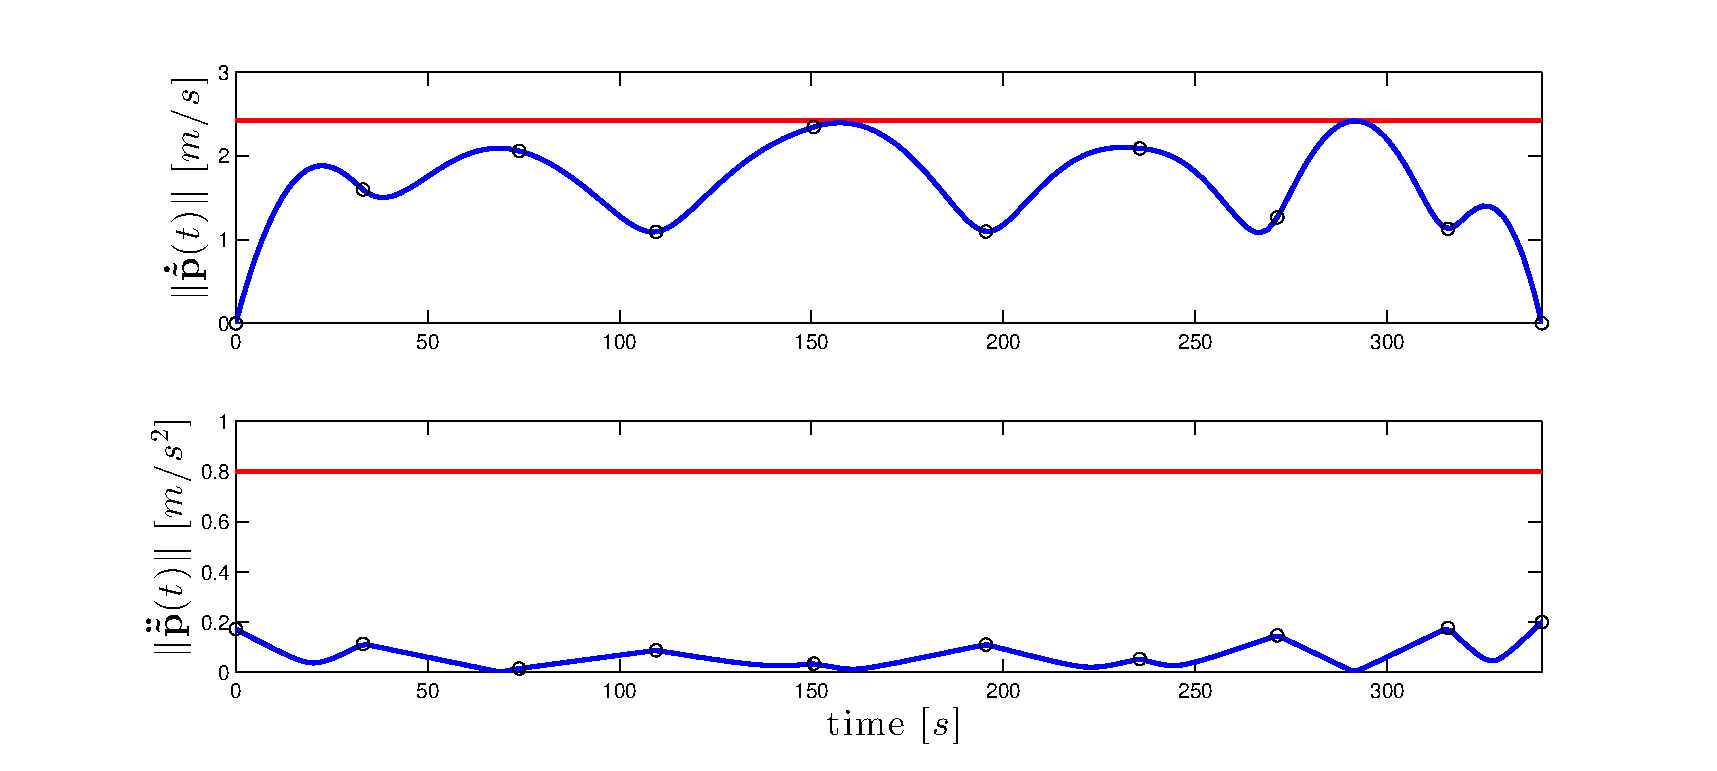
\includegraphics[width = 0.9\textwidth]{graphics/constantTimeScaling3cp_road.eps}
  \caption{From a constant time scaling resulting velocity and acceleration for the \textit{road} trajectory generated with cubic splines, in red the system constraints}
  \label{fig:constantTimeScaling3cp_road}
\end{figure}



\subsubsection{A Simple Non Linear Approach}
As described in \ref{subsec:boundary conditions}, polynomials of at least quartic degree would be necessary to set the boundary conditions of the second derivative ${\bf \ddot{\tilde{p}}}(t)$ when using constant time scaling. As an alternative (not only for cubic splines), non linear time parametrization can be used. A simple approach is to replace the beginning and ending of the linear time parametrization $u(t)=\lambda t$ by a polynomial of higher degree\footnote{See \cite{doessegger} and \cite{biagiotti} for more advanced approaches.}.

We use cubic time parametrizations for the intervals $u_0$ to $u_1$ and $u_{n-1}$ to $u_n$ as illustrated in figure \ref{fig:non_linear_time}.

\begin{figure}[h]
    \centering
    \includegraphics[width = 0.8\textwidth]{graphics/constantTimeScaling_adoptedBoundaries.eps}
    \caption{Visualization of the constant time scaling with adopted boundaries.}
    \label{fig:non_linear_time}
\end{figure}

Like that, $\ddot{\tilde{{\bf p}}}(t_0)$ and $\ddot{\tilde{{\bf p}}}(t_n)$ can be set to zero if 
\begin{equation*}
\dot{u}(t_0)=\dot{u}(t_n)=\frac{d{\bf p}}{du}\Bigm|_{u=u_0}=\frac{d{\bf p}}{du}\Bigm|_{u=u_n}=0
\end{equation*}

With these conditions, $u(t_0)=u_0$, $u(t_n)=u_n$ and the equations resulting from continuous boundary conditions, the following motion law is obtained by solving the nonlinear set of equations\footnote{E.g. using \textsc{Wolfram Mathematica}.}

\begin{equation}
u(t) =
\begin{cases}
a_0 t^3 + b_0 t^2 + c_0 t + d_0 & \quad 0 < t \leq t_1\\
\lambda t + \tilde{d} & \quad t_1 < t \leq t_{n-1}\\
a_{n-1} t^3 + b_{n-1} t^2 + c_{n-1} t + d_{n-1} & \quad t_{n-1} < t \leq t_n
\end{cases}
\end{equation}

whereas

\begin{align*}
a_0 &= \frac{\lambda}{9t_1^2} , \quad
b_0 = \frac{\lambda}{3t_1} , \quad
c_0 = 0 , \quad
d_0 = 0 , \quad
\tilde{d} = - \frac{5}{9}\lambda t_1 , \\
a_{n-1} &= -\frac{4 \lambda^3}{27 (\tilde{d} + \lambda t_{n-1} - u_n)^2} , \quad
b_{n-1} = \frac{4 \lambda^3 t_{n-1}}{9 (\tilde{d} + \lambda t_{n-1} - u_n)^2} , \\
c_{n-1} &= \frac{\lambda (9 \tilde{d}^2 + 18 \lambda \tilde{d} t_{n-1} + 5 \lambda^2 t_{n-1}^2 - 18 \tilde{d} u_n - 18 \lambda t_{n-1} u_n + 
   9 u_n^2)}{9 (\tilde{d} + \lambda t_{n-1} - u_n)^2} , \\
d_{n-1} &= \frac{27 \tilde{d}^3 + 54 \lambda \tilde{d}^2 t_{n-1} + 27 \lambda^2 \tilde{d} t_{n-1}^2 + 4 \lambda^3 t_{n-1}^3 - 
 54 \tilde{d}^2 u_n - 54 \lambda \tilde{d} t_{n-1} u_n + 27 \tilde{d} u_n^2}{27 (\tilde{d} + \lambda t_{n-1} - u_n)^2} , \\
t_n &= \frac{-3 \tilde{d} - \lambda t_{n-1} + 3 u_n}{2 \lambda}
\end{align*}

%\pagebreak
\section{Controller Implementation}
\label{sec:controllerImplementation}
A trajectory controller and two commonly used path tracking controllers\footnote{\cite{snider} provides a good overview over various approaches.} are tested to follow the defined trajectories. The \textit{trajectory following} controller supplies the system's position controller, described in \cite{meiermueri}, with a feed forward reference signal. Although it delivers good results for the ideal case, the tracking gets worse for the non perfect model case. The \textit{pure pursuit} controller, which is based on a lookahead point as well as the \textit{cross track error} controller dynamically react on model uncertainties and yield therefore more robust and accurate path tracking results.

\subsection{Trajectory Following}
Assuming a perfect model and a trajectory considering all system constraints\footnote{I.e. saturations of $\dot{r}(t)$ and its derivatives, see section \ref{subsec:systemConstraints}.} the position $r\left(t\right)$ of the system can be assumed to be equal to the trajectory $\tilde{p}(t)$ at any time. Therefore, a straight forward way of a trajectory controller is to follow the trajectory $\tilde{p}(t)$ for every time $t$. The idea is illustrated in figure \ref{fig:scene_trajectoryFollowing}. This trajectory controller yields accurate tracking in a safe environment \cite{doessegger}.
\\
A position PI controller with feed forward terms for velocity and acceleration can therefore be used with the reference input

\begin{equation}
  [{\bf{r}}_{ref}(t), \; {\bf\dot{r}}_{ref}(t), \; {\bf\ddot{r}}_{ref}(t)]^T = [{\bf\tilde{p}}(t), \; {\bf\dot{\tilde{p}}}(t), \; {\bf\ddot{\tilde{p}}}(t)]^T
\end{equation}

The controller scheme is shown in figure \ref{fig:trajectoryfollowing}. 

%$\left[ \begin{array}{c} {\bf r}(t) \\ {\bf \dot{r}}(t) \end{array} \right]$
\begin{figure}[H]
    \centering
    \def\svgwidth{0.4\columnwidth}
    \input{graphics/controller/scene_trajectoryFollowing.pdf_tex}
    \caption{Trajectory Following. The reference input $[{\bf\tilde{p}}(t), \; {\bf\dot{\tilde{p}}}(t), \; {\bf\ddot{\tilde{p}}}(t)]^T$ is predefined by the trajectory for every time $t$. The value of the parameter $t$ of the trajectory is equal to the current time.}
    \label{fig:scene_trajectoryFollowing}
\end{figure}

\begin{figure}[H]
    \centering
    \def\svgwidth{\columnwidth}
    \input{graphics/controller/controller_trajectoryFollowing.pdf_tex}
    \caption{Trajectory Following Controller Scheme. The reference input for the closed loop position controller is a function of the current time $t$ only.}
    \label{fig:trajectoryfollowing}
\end{figure}

%\begin{figure}[h]
%    \centering
%    \includegraphics[width = \textwidth]{trackings/figure_2D_road_SplineDegree3_trajectoryFollowing_Disturbance_0}
%  \hfill
%  \caption{BLA dynamics}
%  \label{fig:trajFoll_dynamics}
%\end{figure}

%\begin{figure}[h]
%    \centering
%    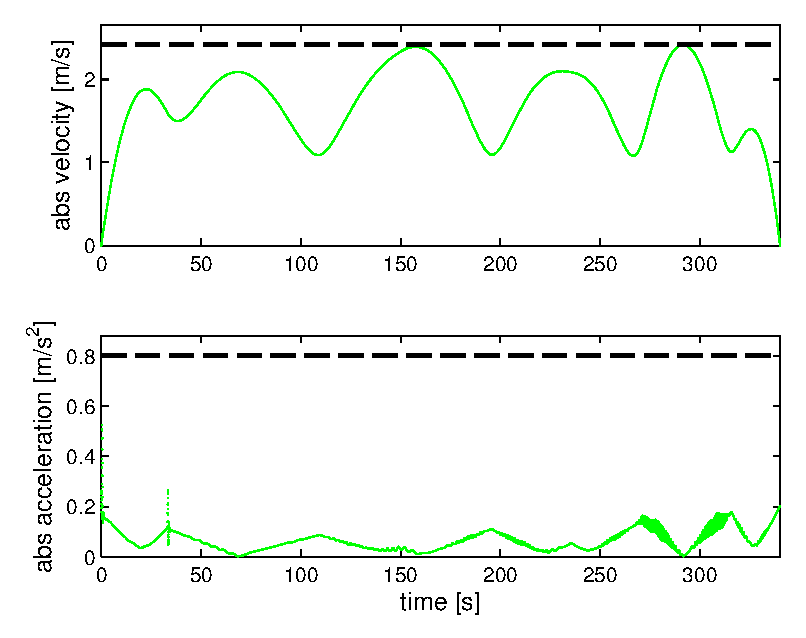
\includegraphics[width = 0.8\textwidth]{trackings/figure_1D_road_SplineDegree3_trajectoryFollowing_Disturbance_0}
%  \hfill
%  \caption{BLA dynamics}
%  \label{fig:trajFoll_dynamics}
%\end{figure}

\subsection{Pure Pursuit Controller}
\label{sub:pure_pursuit}
Another commonly used controller to track paths is \textit{pure pursuit} \cite{snider}. This technique is mainly used for path tracking while having a constant tangential velocity. The idea of using a lookahead point was adapted for trajectory control. To do that, the lookahead point ${\bf \tilde{p}}(t_{cl}+\Delta T)$ is set on the trajectory in front\footnote{$\Delta T = \SI{1}{second}$ proofed to be reasonable for all considered conditions.} of the current closest position ${\bf \tilde{p}}(t_{cl})$.
\begin{equation}
{\bf \tilde{p}}(t_{cl}+\Delta T) = {\bf \tilde{p}}(t_{cl}) + \Delta T \cdot {\bf\dot{ \tilde{p}}}(t_{cl}) + \frac{1}{2} \Delta T^2 \cdot {\bf\ddot{ \tilde{p}}}(t_{cl}) + \mathcal{O}(\Delta T^3)
\end{equation}
Therefore, the controller considers the full dynamics of the trajectory, i.e. ${\bf \tilde{p}}(t)$ and all its derivatives\footnote{This is a simple and robust alternative to any derivative controller.}.
Figure \ref{fig:scene_purePursuit} represents the controller's functionality. The control scheme can be seen in figure \ref{fig:purePursuit}. Actually, the inner control block is a velocity controller only. The reference velocity is given by
\begin{equation}
{\bf \dot{r}}_{ref}(t) = \frac{{\bf \tilde{p}}(t_{cl}+\Delta T)-{\bf r}(t)}{\Delta T}
\end{equation}


%$ {\bf \dot{r}}_{ref}(t) $
\begin{figure}[H]
    \centering
    \def\svgwidth{0.5\columnwidth}
    \input{graphics/controller/scene_purePursuit.pdf_tex}
    \caption{Pure Pursuit. The reference velocity is given by the difference between the actual position and a lookahead point defined by the trajectory's closest point shifted by $\Delta T$ ahead.}
    \label{fig:scene_purePursuit}
\end{figure}

\begin{figure}[H]
    \centering
    \def\svgwidth{\columnwidth}
    \input{graphics/controller/controller_purePursuit.pdf_tex}
    \caption{Pure Pursuit Controller Scheme. The position feedback is closed by defining the lookahead point depending on the closest point of the trajectory.}
    \label{fig:purePursuit}
\end{figure}

%\begin{figure}[H]
%  \begin{minipage}[t]{0.32\textwidth}
%    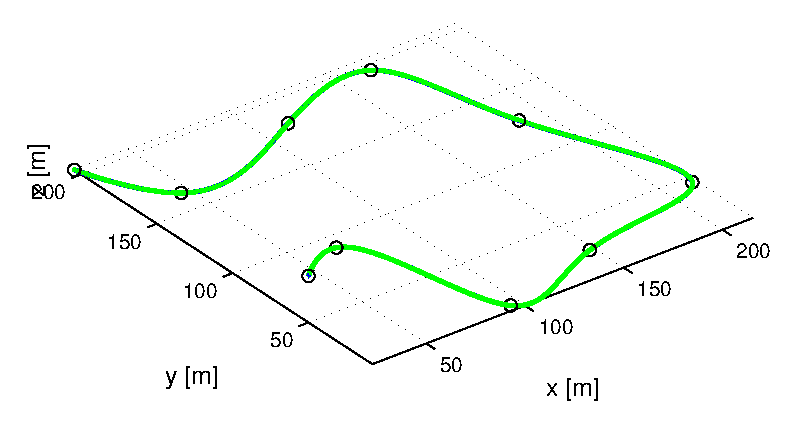
\includegraphics[width = \textwidth]{trackings/figure_3D_road_SplineDegree3_purePursuit_Disturbance_0}
%  \end{minipage}
%  \hfill
%  \begin{minipage}[t]{0.32\textwidth}
%    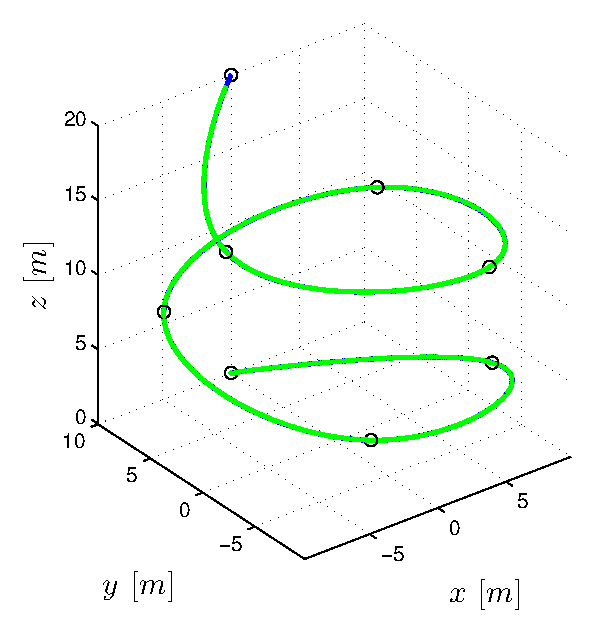
\includegraphics[width = \textwidth]{trackings/figure_3D_helix_SplineDegree3_purePursuit_Disturbance_0}
%  \end{minipage}
%  \hfill
%  \begin{minipage}[t]{0.32\textwidth}
%    \includegraphics[width = \textwidth]{trackings/figure_3D_agile_SplineDegree3_purePursuit_Disturbance_0}
%  \end{minipage}
%  \caption{BLA pure pursuit}
%  \label{fig:purePursuit_tracking}
%\end{figure}
%
%\begin{figure}[H]
%  \begin{minipage}[t]{0.32\textwidth}
%    \includegraphics[width = \textwidth]{trackings/figure_3D_road_SplineDegree3_purePursuit_Disturbance_1}
%  \end{minipage}
%  \hfill
%  \begin{minipage}[t]{0.32\textwidth}
%    \includegraphics[width = \textwidth]{trackings/figure_3D_helix_SplineDegree3_purePursuit_Disturbance_1}
%  \end{minipage}
%  \hfill
%  \begin{minipage}[t]{0.32\textwidth}
%    \includegraphics[width = \textwidth]{trackings/figure_3D_agile_SplineDegree3_purePursuit_Disturbance_1}
%  \end{minipage}
%  \caption{BLA pure pursuit and here with wind}
%  \label{fig:purePursuit_tracking}
%\end{figure}

\subsection{Cross Track Error Controller}
The idea of the \textit{cross track error} controller is to directly reduce the cross track error distance\footnote{The distance normal to the path. Compare figure \ref{fig:scene_crossTrack}.}. This practise is also used in navy \cite{williams} or for wheeled robots \cite{deluca}. The actual operation is very similar to the one in \textit{trajectory following}, but instead of considering the trajectory's current time, here, the reference input time is defined by the closest point of the trajectory. Afterwards, the same position controller as mentioned above is used to track the reference state. Figure \ref{fig:scene_crossTrack} illustrates the choise of the reference input for the controller. The control scheme is shown in figure \ref{fig:crossTrack}.

%$\left[ \begin{array}{c} {\bf \tilde{p}}(t) \\ {\bf \dot{\tilde{p}}}(t) \\ {\bf \ddot{\tilde{p}}}(t) \end{array} \right]$
\begin{figure}[H]
    \centering
    \def\svgwidth{0.5\columnwidth}
    \input{graphics/controller/scene_crossTrack.pdf_tex}
    \caption{Cross Track Error. The reference point is the nearest point on the trajectory.}
    \label{fig:scene_crossTrack}
\end{figure}


\begin{figure}[H]
    \centering
    \def\svgwidth{\columnwidth}
    \input{graphics/controller/controller_crossTrack.pdf_tex}
    \caption{Cross Track Error Controller Scheme. The value of the trajectories time stamp $t_{cl}$ of the closest point is generally not equal the current time $t$.}
    \label{fig:crossTrack}
\end{figure}


%\begin{figure}[H]
%  \begin{minipage}[t]{0.32\textwidth}
%    \includegraphics[width = \textwidth]{trackings/figure_3D_road_SplineDegree3_crossTrack_Disturbance_0}
%  \end{minipage}
%  \hfill
%  \begin{minipage}[t]{0.32\textwidth}
%    \includegraphics[width = \textwidth]{trackings/figure_3D_helix_SplineDegree3_crossTrack_Disturbance_0}
%  \end{minipage}
%  \hfill
%  \begin{minipage}[t]{0.32\textwidth}
%    \includegraphics[width = \textwidth]{trackings/figure_3D_agile_SplineDegree3_crossTrack_Disturbance_0}
%  \end{minipage}
%  \caption{BLA cross track}
%  \label{fig:crossTrack_tracking}
%\end{figure}
%
%\begin{figure}[H]
%  \begin{minipage}[t]{0.32\textwidth}
%    \includegraphics[width = \textwidth]{trackings/figure_3D_road_SplineDegree3_crossTrack_Disturbance_1}
%  \end{minipage}
%  \hfill
%  \begin{minipage}[t]{0.32\textwidth}
%    \includegraphics[width = \textwidth]{trackings/figure_3D_helix_SplineDegree3_crossTrack_Disturbance_1}
%  \end{minipage}
%  \hfill
%  \begin{minipage}[t]{0.32\textwidth}
%    \includegraphics[width = \textwidth]{trackings/figure_3D_agile_SplineDegree3_crossTrack_Disturbance_1}
%  \end{minipage}
%  \caption{BLA cross track with wind}
%  \label{fig:crossTrackWind_tracking}
%\end{figure}

\section{Results}
\label{sec:results}

A model of system \textsc{Skye} has been elaborated in \cite{weichart} and was available as \textsc{Matlab Simulink} model to test the controller performance. The controllers described above were tested within the experimental design notified in section \ref{sec:experimental design}. If not mentioned explicitly, the shown trajectories are designed using cubic splines and centripetal parametrization. The results are presented for perfect model estimation as well as for the case of wind disturbances and model uncertainties\footnote{Note, that for all cases perfect measurement feedback was used, i.e. the simulation does not include measurement noise.}. Furthermore the correlation between different parameters is shown. Further results can be found in the appendix (\ref{cha:appendix}). 
The occurring accelerations ($J_5$) as well as the percentage of reached trajectory ($J_6$) remain nearly the same for all shown results.

\subsection{Perfect Model Estimation}
\label{sub:results_perfect_model}

The three trajectory controllers were tested with the given waypoint samples. Figure \ref{fig:results_perfect_model} shows their tracking. The performance difference between them is minimal as it can be seen from the results listed in table \ref{tab:results_perfect_model}. In comparison to the systems characteristic size (diameter \SI{2.7}{\meter}) the deviations between trajectory and trace are extremely small, i.e. less than 1\% of the characteristic size. The average acceleration is nearly the same for all controllers. It is given by the shape of the trajectory.

\begin{table}[h]
\begin{center}
 \begin{tabular}{lll|rrr}
 \hline
 Controller & Criterion & Unit & \textit{Road} & \textit{Helix} & \textit{Agile} \\ \hline \hline
 Trajectory Following & Av. Dev. & $[\si{\meter}]$ & 0.007 & 0.017 & 0.014 \\
 Pure Pursuit         & Av. Dev. & $[\si{\meter}]$ & 0.007 & 0.009 & 0.017 \\
 Cross Track          & Av. Dev. & $[\si{\meter}]$ &  0.007 & 0.007 & 0.006 \\
    
 Trajectory Following & Av. Acc. & $[\si{\meter\per\square\second}]$ & 0.029 & 0.174 & 0.137 \\
 Pure Pursuit         & Av. Acc. & $[\si{\meter\per\square\second}]$ & 0.031 & 0.159 & 0.128 \\
 Cross Track          & Av. Acc. & $[\si{\meter\per\square\second}]$ & 0.029 & 0.159 & 0.126 \\
 
 Trajectory Following & Reached & $[\si{\percent}]$ & 100 & 100 & 100 \\
 Pure Pursuit         & Reached & $[\si{\percent}]$ &  99 &  97 &  98 \\
 Cross Track          & Reached & $[\si{\percent}]$ &  97 &  97 &  97 \\
 \hline
 \end{tabular}
 \caption{Results of the three controllers using perfect model estimation}\vspace{1ex}
 \label{tab:results_perfect_model}
\end{center}
\end{table}


\subsection{Wind Disturbance}
\label{sub:results_wind_disturbance}

The same simulations have been conducted with wind disturbance. Wind forces based on a constant wind velocity of \SI{1}{\meter\per\second} in positive x-direction have been added to the scenes\footnote{The maximum possible relative velocity of the simulated system is about \SI{2.4}{\meter\per\second}.}. To enable to eventually see the effect of the upcoming wind, the disturbance is added 10 seconds after the simulation's start\footnote{The simulation lengths are about \SI{340}{\second} (\textit{road}), \SI{65}{\second} (\textit{helix}) and \SI{80}{\second} (\textit{road}) respectively.}. \\
Figure \ref{fig:results_wind_disturbance} shows the tracking reached by the three controllers. The resulting performance values are listed in table \ref{tab:results_wind_disturbance}. While \textit{pure pursuit} and \textit{cross track error} control still result in small deviation\footnote{They are still about factor 20 smaller than the characteristic size of \textsc{Skye}.} the deviation has grown to a considerable big scale for \textit{trajectory following} as it can be seen in figure \ref{fig:result_wind_trajfoll}.

\begin{figure}[H]
  \centering
  \begin{minipage}[t]{0.48\textwidth}
	\includegraphics[width=\textwidth]{graphics/trackings/figure_3D_helix_SplineDegree3_trajectoryFollowing_Disturbance_0.eps}
  \end{minipage}
  \hfill
  \begin{minipage}[t]{0.48\textwidth}
	\includegraphics[width=\textwidth]{graphics/trackings/figure_3D_helix_SplineDegree3_trajectoryFollowing_Disturbance_1.eps}
  \end{minipage}
	\caption{Result of tracking \textit{agile} waypoints using \textit{trajectory following}; \textbf{Left}: Perfect model estimation; \textbf{Right}: Wind disturbance}
	\label{fig:result_wind_trajfoll}
\end{figure}



\textit{Cross track error} control slightly scores better than \textit{pure pursuit}. Again, the accelerations are similar for all controllers. While \textit{trajectory following} reaches the end of the trajectory almost exact within the given time $T_p$, the path tracking based trajectory controllers are slower and will remain at \SIrange{86}{96}{\percent} of the trajectories length $L_p$ at the time $T_p$. \\
Compared to the results of perfect modelling (section \ref{sub:results_perfect_model}), the deviations when using \textit{trajectory following} get worse by factor \numrange{10}{200} and by the two accurate controllers \numrange{5}{10} times. The accelerations are comparable to the ideal case.

\begin{table}[h]
\begin{center}
 \begin{tabular}{lll|rrr}
 \hline
 Controller & Criterion & Unit & \textit{Road} & \textit{Helix} & \textit{Agile} \\ \hline \hline
 Trajectory Following & Av. Dev. & $[\si{\meter}]$ & 1.783 & 0.606 & 0.111 \\
 Pure Pursuit         & Av. Dev. & $[\si{\meter}]$ & 0.079 & 0.098 & 0.037 \\
 Cross Track          & Av. Dev. & $[\si{\meter}]$ & 0.034 & 0.061 & 0.023 \\

 Trajectory Following & Av. Acc. & $[\si{\meter\per\square\second}]$ & 0.031 & 0.191 & 0.138 \\
 Pure Pursuit         & Av. Acc. & $[\si{\meter\per\square\second}]$ & 0.031 & 0.136 & 0.121 \\
 Cross Track          & Av. Acc. & $[\si{\meter\per\square\second}]$ & 0.028 & 0.140 & 0.120 \\
 
 Trajectory Following & Reached & $[\si{\percent}]$ & \ktilde100 & \ktilde100 & \ktilde100 \\
 Pure Pursuit         & Reached & $[\si{\percent}]$ &  96 &  86 &  96 \\
 Cross Track          & Reached & $[\si{\percent}]$ &  94 &  89 &  95 \\
 \hline
 \end{tabular}
 \caption{Results of the three controllers with wind disturbance}\vspace{1px}
 \label{tab:results_wind_disturbance}
\end{center}
\end{table}


\subsection{Model Uncertainties}
\label{sub:results_model_uncertainties}

The simulations were repeated by designing the trajectories by using system constraints with a safety factor reduced to less than one, i.e. to \num{0.8}. Therefore, the trajectory overestimates the system's actuation possibilities. \\
The tracking of all controllers is shown in figure \ref{fig:results_model_uncertainties}. The numerical results are listed in table \ref{tab:results_model_uncertainties}. The deviation of \textit{trajectory following} control is considerable larger than of the two other ones. \textit{Pure pursuit} even tops the \textit{cross track error} results in this case. The average accelerations are slightly higher when using \textit{trajectory following}.
%Contrary to the \textit{trajectory following} which heads to the actual end of the trajectory by $T_p$, \textit{pure pursuit} and \textit{cross track error} will lead to \SIrange{86}{93}{\percent} of the circuit's length.
\\
In comparison to the ideal case, the deviations of the accurate controllers get worse \numrange{2}{10} times. \textit{Trajectory following} leads to deviations \numrange{50}{400} times larger than for perfect modelling. Average accelerations grew by factors less than \num{2}.

\begin{table}[H]
\begin{center}
 \begin{tabular}{lll|rrr}
 \hline
 Controller & Criterion & Unit & \textit{Road} & \textit{Helix} & \textit{Agile} \\ \hline \hline
 Trajectory Following & Av. Dev. & $[\si{\meter}]$ & 3.228 & 1.628 & 0.838 \\
 Pure Pursuit         & Av. Dev. & $[\si{\meter}]$ & 0.049 & 0.026 & 0.036 \\
 Cross Track          & Av. Dev & $[\si{\meter}]$ &  0.092 & 0.044 & 0.058 \\
    
 Trajectory Following & Av. Acc. & $[\si{\meter\per\square\second}]$ & 0.066 & 0.234 & 0.234 \\
 Pure Pursuit         & Av. Acc. & $[\si{\meter\per\square\second}]$ & 0.045 & 0.210 & 0.182 \\
 Cross Track          & Av. Acc. & $[\si{\meter\per\square\second}]$ & 0.047 & 0.220 & 0.192 \\
 
 Trajectory Following & Reached & $[\si{\percent}]$ & \ktilde100 & \ktilde90 & \ktilde100 \\
 Pure Pursuit         & Reached & $[\si{\percent}]$ &  86 &  90 &  86 \\
 Cross Track          & Reached & $[\si{\percent}]$ &  87 &  93 &  89 \\
 \hline
 \end{tabular}
 \caption{Results of the three controllers with underestimated trajectory constraints}\vspace{1px}
 \label{tab:results_model_uncertainties}
\end{center}
\end{table}

\subsection{Data Correlation}
Within the gathered data of the tracking with ideal conditions (section \ref{sub:results_perfect_model}) and considering all introduced parametrizations and spline degrees from section \ref{sec:splines} a data set of 108 items was analyzed for correlation\footnote{The additional cases with non perfect modelling ($3\cdot 108$ items with wind and/or model uncertainties) will not be shown. Indeed, the correlations cannot be seen there explicitly.}. Some correlating results could be observed. \\
Figure \ref{fig:correlation_time_acc} shows the relation between the given time $T_p$ for the trajectory and the average acceleration $J_5$ occurring on the system. The result is trivial, as the less time is given to follow the waypoints, the higher gets the acceleration. The dependence on the used parametrization is different for the different waypoints, whereas higher spline degrees (quartic and quintic) yield to slightly smaller time $T_p$ and acceleration $J_5$ than lower degree (cubic) consequently. Although, these differences are very small. \\
In figure \ref{fig:correlation_invdev_acc} the correlation between the average deviation $J_4$ and the average acceleration $J_5$ occurring on the system are shown for the \textit{road} waypoints\footnote{Figure \ref{fig:correlation_invdev_acc_all_circuits} includes all waypoint samples. The correlations are similar but much more disturbed.}. As expected, higher accelerations correlates with higher deviations. Cubic splines yield to worse performance than quartic and quintic, which are nearly the same.
\\ Note that cubic splines are restricted to \num{4} boundary conditions and therefore start and end with accelerations unequal zero. 

\begin{figure}[H]
  \begin{minipage}[t]{0.48\textwidth}
    \includegraphics[width = \textwidth]{correlation/Control_Correlation_Time_Acc_Parametrization}
  \end{minipage}
  \hfill
  \begin{minipage}[t]{0.48\textwidth}
    \includegraphics[width = \textwidth]{correlation/Control_Correlation_Time_Acc_SplineDegree}
  \end{minipage}
  \caption{Correlation between trajectory time length $T_p$ and average accelerations on trace on a double logarithmic plot. Although the overall correlation can be seen clear, the dependency of the trajectory's degree or parametrization is minimal. {\bf Left}: Different waypoint parametrizations uniform (black), chord length (blue), arc length (green) and centripetal (red). {\bf Right}: Different spline degrees cubic (green), quartic (cyan) and quintic (magenta).}
  \label{fig:correlation_time_acc}
\end{figure}

\begin{figure}[H]
  \begin{minipage}[t]{0.48\textwidth}
    \includegraphics[width = \textwidth]{correlation/Control_Correlation_InvDev_Acc_Parametrization}
  \end{minipage}
  \hfill
  \begin{minipage}[t]{0.48\textwidth}
    \includegraphics[width = \textwidth]{correlation/Control_Correlation_InvDev_Acc_SplineDegree}
  \end{minipage}
  \caption{Correlation between average path deviation and average accelerations. Data points from \textit{road} waypoints. {\bf Left}: Different waypoint parametrizations uniform (black), chord length (blue), arc length (green) and centripetal (red). {\bf Right}: Different spline degrees cubic (green), quartic (cyan) and quintic (magenta).}
  \label{fig:correlation_invdev_acc}
\end{figure}

\pagebreak
\section{Discussion}
\label{sec:discussion}

%\textit{The almost endless field of trajectories represents the individual needs for for trajectories within different situations. Before considering steering by waypoints, the criteria for a good fitting trajectory have to be elaborated. This can be very case-specific, as it depends not only on available system's actuation, but also on the way one sets the waypoints. The holonomic design of the system has to be considered as well as environmental obstacles at the scene. Suitable trajectory controllers will handle aaaaaaaaaaa\\ Therefore, geometrical design of the path has mainly to be considered. Dynamical aspect of the trajectory depends largely on the used controller..} HELLO?

The almost endless field of trajectory control represents the manifold needs for trajectories in different application fields. 
%While the underlying spline theories have theirs roots in automobile industry XXXX \cite{deboor}, they can be adopted for any use.
Even to control UAVs no throughout good or bad trajectory algorithms can be named. Their quality rather has to be rethought for any specific use. Therefore, as for every optimization problem, it is fundamental to properly define rating criteria before thinking of any trajectories. \\
For \textsc{Skye} tight waypoint tracking was considered more important than for instance time minimization or smoothness. Therefore cubic splines based on centripetal parametrized waypoints result in good performance for most considerable waypoint samples.
For sake of simplicity, even a linear time parametrization considering the system's actuation saturations can be used to yield sufficient results. \\
Independent on the choice how to generate the trajectories, proper controllers influence the actual performance of the system in case of non perfect modelling. As the presented trajectory algorithms cannot consider e.g. current environmental conditions as wind, it is recommended to use time-variant trajectory controllers\footnote{We do not use the name \textit{path tracking} as using time parametrized trajectories allow to strictly obtain system constraints. Path tracking is mainly restricted to nonholonomic vehicles cruising at constant speed as boats \cite{williams}, planes or wheeled systems \cite{deluca}, \cite{snider}.} to maintain best possible trajectory tracking.

 \cleardoublepage
 %!TEX root = Bericht.tex
\chapter{Conclusion}
%\textit{
%What is the strongest and most important statement that you can make from your observations? 
%If you met the reader at a meeting six months from now, what do you want them to remember about your paper? 
%Refer back to problem posed, and describe the conclusions that you reached from carrying out this investigation, summarize new observations, new interpretations, and new insights that have resulted from the present work.
%Include the broader implications of your results. 
%Do not repeat word for word the abstract, introduction or discussion.}\\
%\textit{To summarize
%� What you researched� Nature of your main arguments� How you researched it� What you discovered� What pre-existing views were challenged
%2. To provide an overview of 
%The new knowledge or information discovered� The significance of your research (where is it new?)� The limitations of your thesis (concepts, data)� Speculation on the implications of these limitations� Areas for further development and research(alternative data sets; links with other fields; differentmethod applied to same data)
%The �1 Must� and the �3 Ideals�
%You
%must 1. Make a clear and concise statement of theoriginal contribution to knowledge found in your thesis.Ideally 
%you should aspire to1. Show links between the key ideas spread acrosschapters2. Show your commitment to and enthusiasm for academic research3. Leave a positive impression with the examiner .\\
%Avoid claiming findings that you have not proventhroughout your thesis� Avoid introducing new data� Avoid hiding weaknesses or limitations in your thesis(make a virtue of showing strong analytical skills and self-critique by discussing the limitations--but don�t gooverboard on this!)�  Avoid making practical recommendations (e.g. for policy).If you must include them put them in an appendix.� Avoid being too long (repetitive) or too short (sayingnothing of importance)
%Sample Conclusion Structure (1)
%One paragraph stating what you researched and what your original contribution to the field is�then break into sections� One section on what you researched and how you did it� One section on what are the main findings were� showinglinks across chapters (this explains why you chose thestructure you did)� One section on possible areas for future research� Final section reminding readers of the original contributionand significance of your research to your field.
%Sample Conclusion Structure (2)
%One paragraph stating what you researched and what your original contribution to the field is�then break into sections� Main finding 1 (subsections on how you arrived at thisfinding and how it challenges previous research)� Main finding 2 (subsections on how you arrived at thisfinding and how it challenges previous research)� Main finding 3 (subsections on how you arrived at thisfinding and how it challenges previous research)� One section on potential leads to openings for further research resulting from your research� Final section reminding readers of the original contributionand significance of your research to your field.
%Concluding Conclusion
%Be enthused by the prospect of writing your conclusion� �It�s downhill from here�!�To avoid the concluding chapter shock�
%� Start writing notes of content for potentialsections of your conclusion as you write other chapters�add bits in as you think of them� If you find a succinct quote that encapsulatescommon misunderstandings about your fieldthen use it at the start to bounce off.
%}
%


%old---------------------------------
%In this Thesis, a HMI, tailored to the needs of \textsc{Skye} has been developed. This ranges from defining control modes for six DOF, planing feasible trajectories to implementing these ideas to form a complete HMI. As for the trajectory planning existing solutions were adopted, the combination of touchscreen with a 3D mouse to control \textsc{Skye} is a new, so far unseen approach.  However, in order to realize all ideas for an intuitive HMI, a lot of challenges had to be met.
%
%\paragraph{Challenges}
%Working on a real project as a team means also finding interfaces for the different domains of the project as well as finding interfaces for the workload the different team members are taking. For the HMI which is almost connected to everything of the project,  this meant that the options for choosing the hardware and software were quite limited. Nevertheless a compact and convenient solution was found in discussions with the control and communication section of team \textsc{Skye}.\\
%Taking existing solution brings with it, that these solutions also have to be understood thoroughly. Otherwise it is impossible to adopt it reasonably. E.g. the source code of \textsc{QGroundControl} had to be analyzed and this proved to be not that easy as it is a far developed code contributed by many different programmers.
%%it was someone else's code. However, as time passes by, you get used to it.\\
%Developing a HMI for a system which itself is not yet fully developed was also a challenge. Numerous days were invested in other domains of the project, in order the make the whole system run and especially to make the HMI working properly with it. Especially the integration of an alpha version FMU required thousand of tests till it was a stable running system. 
%
%
%\paragraph{Maturity of the Solutions} Due to a not completely mature prototype and due to lack of time, not all ideas could be tested on the real system.
%While the finished \textit{test phase}, \textit{direct} and \textit{assisted control} modes proved their functionality on the real system, the \textit{half} and \textit{full automatic} control modes still need to be tested.
%However, there is already a simulation of the \textit{half automatic} control mode running on the GUI and it is assumed that only the controller and the state estimation would have to be adopted to make it work.
%This is not like the situation of the \textit{full automatic} control mode.
%It is still far from maturity as only a \textsc{Matlab} simulation of it exists.
%
%
%\paragraph{Open Ideas} As mentioned above is the \textit{full automatic} control not yet elaborated in detail. However, it is supposed that a complete automatic mode would boost the application field of \textsc{Skye} and therefore it is suggested to realize this mode in a further step of project \textsc{Skye}.\\
%Right now the generated trajectories are only optimized to not exceed the system abilities. In a further step they could be optimized for time or energy consumption.\\
%Although a widget for the control of the onboard cameras was developed, it was never put in action. The same applies to a battery widget which would constantly display the battery level of all three accumulators. Having these widgets work would extend the pilot's control over \textsc{Skye}.
%
%\paragraph{} Looking back on the developed HMI and the source code of the software, a lot of things would be done in a more effective and easier way. Yet this is not surprising as a lot of learning experience was gained. Even Lorenz Meier, the skilled programmer who developed \textsc{QGroundControl}, told us: "You know what I did once I had finished the source code of \textsc{QGroundControl}? - I wrote it all again."  %However, the general concept of the HMI with tablet, 3D mouse and trajectory planning would not be changed, which might be surprising.
%However, the general concept of the HMI with tablet, 3D mouse and trajectory planning proved to be the right choice.






%new---------------------------------
In this Thesis, a HMI, tailored to the needs of \textsc{Skye} has been developed. This ranges from defining control modes for six DOF, planing feasible trajectories to implementing these ideas to form a complete HMI. As for the trajectory planning existing solutions were adopted, the combination of touchscreen with a 3D mouse to control \textsc{Skye} is a new, so far unseen approach.  However, in order to realize all ideas for an intuitive HMI, a lot of challenges had to be met.

\paragraph{Challenges}
Working on a real project as a team means also finding interfaces for the different domains of the project as well as finding interfaces for the workload the different team members are taking. For the HMI which is almost connected to everything of the project,  this meant that the options for choosing the hardware and software were quite limited. Nevertheless a compact and convenient solution was found in discussions with the control and communication section of team \textsc{Skye}. Developing a HMI for a system which itself is not yet fully developed was also a challenge. Numerous days were invested in other domains of the project, in order the make the whole system run and especially to make the HMI working properly with it. Especially the integration of an alpha version FMU required thousand of tests till it was a stable running system. 


\paragraph{HMI's Maturity and Open Ideas} 
Due to a not completely mature prototype and due to lack of time, not all ideas and implementations could be tested on the real system. While the finished \textit{test phase}, \textit{direct} and \textit{assisted control} modes proved their functionality on the real system, the \textit{half} and \textit{full automatic} control modes still need to be tested. However, there is already a simulation of the \textit{half automatic} control mode running on the GUI and it is assumed that only the controller and the state estimation would have to be adopted to make it work. For the \textit{full automatic} control mode only a \textsc{Matlab} simulation of it exists and it still would need to be tested properly. Yet it is supposed that a complete \textit{full automatic} mode  would boost the application field of \textsc{Skye} and therefore it is suggested to realize this mode in a further development step.
Although a widget for the control of the onboard cameras was developed, it was never put in action. The same applies to a battery widget which would constantly display the battery level of all three accumulators. Both could finally not be realized due to unfinished onboard electronics and software. While for the battery widget the transmission of the voltage metering from the motor units to the low lever \textit{Cortex M4} processor was missing, the readout of the camera command mavlink messages was missing in order to have camera  widget work.


\paragraph{Trajectory Tracking} Interpolating the waypoints with a cubic splines based on a centripetal parameterization results in a trajectory suitable for \textsc{Skye}'s applications in built up areas. The linear time scaling used grants feasible trajectories. However, using a more advanced motion law, time or energy consumption could be minimized. For the trajectory tracking it is proposed to use a time-variant trajectory controller, i.e. the elaborated \textit{Pure Pursuit} or the \textit{cross track error} controller. They might not lead to the best time synchrony but for flying in built up areas with environmental disturbances, it is the exact tracking which is most valuable and they yield good results for that.\\

Looking back on the developed HMI and especially on the source code of the software, a lot of things would be done in a more effective and easier way. Yet this is not surprising as a lot of learning experience was gained. However, the general concept and the elaborated solutions for the HMI with tablet, 3D mouse and trajectory planning proved to be the right choice as \textsc{Skye} actually flies with the elaborated HMI.





% ...
%
%---------------------------------------------------------------------------
% Appendix

 \begin{appendix}
 %!TEX root = Bericht.tex

\chapter{Human Machine Interface}
\label{cha:appendix_HMI}
\begin{figure}[H]
    \includegraphics[width = \textwidth]{graphics/HMI/qgc_manual_control_widget.png}
  \caption{\textit{Direct} and \textit{assisted control} widget. For system tests, the engineer can set the system input values directly to the desired value.}
  \label{fig:qgc_manual_control_widget}
\end{figure}

\chapter{Trajectories}
\label{cha:appendix}

\begin{figure}[H]
  \begin{minipage}[t]{0.9\textwidth}
    \includegraphics[width = \textwidth]{graphics/Parameterization345_road_agile.eps}
  \end{minipage}
  \caption{The geometrical appearance of the different parameterizations shown with cubic (top), quartic (middle) and quintic (bottom) splines; uniform (black), chord length (blue), arc length (green), centripetal (red)}
  \label{fig:parameterization_cqq}
\end{figure}

\begin{figure}[H]
  \begin{minipage}[t]{0.9\textwidth}
    \includegraphics[width = \textwidth]{graphics/Parameterization3_road_vel_acc.eps}
  \end{minipage}
  \vfill
    \begin{minipage}[t]{0.9\textwidth}
    \includegraphics[width = \textwidth]{graphics/Parameterization4_road_vel_acc.eps}
  \end{minipage}
  \vfill
    \begin{minipage}[t]{0.9\textwidth}
    \includegraphics[width = \textwidth]{graphics/Parameterization5_road_vel_acc.eps}
  \end{minipage}

  \caption{The dynamic of the different parameterizations in combination with a constant time scaling shown with cubic (top), quartic (middle) and quintic (bottom) splines for the \textit{road} path; uniform (black), chord length (blue), arc length (green), Centripetal (red)}
  \label{fig:parameterization_cqq_dynamic}
\end{figure}

\begin{table}
\begin{center}
 \begin{tabular}{lll|rrrr}
 \hline
 Cubic \textit{Road} & & Unit & Uniform & Chord Length & Arc Length & Centripetal \\ \hline \hline
 Av. Deviation  & $J_1$ & $[\si{\meter}]$    & 3.859 & 4.477 & 4.903 & 3.650 \\
 Av. Curvature & $J_2$ & $[\si{\per\meter}]$ & 0.025 & 0.022 & 0.020 & 0.024 \\
 Av. Acceleration  & $J_3$ & $[\si{\meter\per\square\second}]$ &  0.042 & 0.164 & 0.176 & 0.071 \\
 % CAN IT BE THAT MAXIMUM ACCELERATION IS ABOVE 0.96 ???
 %Max. Acceleration &   & $[\si{\meter\per\square\second}]$ &  0.141 & 1.351 & 1.586 & 0.411 \\
 Time      &   & $[\si{\second}]$ & 388.5 & 322.2 & 334.4 & 340.3 \\
 \hline
 \end{tabular}
 \caption{Comparison of the parametrizations. Static criteria are listed for cubic trajectories using the \textit{road} waypoints.}\vspace{1ex}
 \label{tab:app_results_parameterization_road_cubic}
\end{center}
\end{table}

\begin{table}
\begin{center}
 \begin{tabular}{lll|rrrr}
 \hline
 Cubic \textit{Road} & & Unit & Uniform & Chord Length & Arc Length & Centripetal \\ \hline \hline
 Av. Deviation  & $J_1$ & $[\si{\meter}]$    & 4.043 & 8.452 & 10.963 & 4.774 \\
 Av. Curvature & $J_2$ & $[\si{\per\meter}]$ & 0.050 & 0.036 & 0.032 & 0.047 \\
 Av. Acceleration  & $J_3$ & $[\si{\meter\per\square\second}]$ &  0.062 & 0.449 & 0.506 & 0.139 \\
 Time      &   & $[\si{\second}]$ &  399.5 & 417.3 & 470.6 & 376.4 \\
 \hline
 \end{tabular}
 \caption{Comparison of the parametrizations. Static criteria are listed for quartic trajectories using the \textit{road} waypoints. \textit{Same table than table \ref{tab:results_parameterization_road_quartic}, placed here for completeness.}}\vspace{1ex}
 \label{tab:app_results_parameterization_road_quartic}
\end{center}
\end{table}

\begin{table}
\begin{center}
 \begin{tabular}{lll|rrrr}
 \hline
 Cubic \textit{Road} & & Unit & Uniform & Chord Length & Arc Length & Centripetal \\ \hline \hline
 Av. Deviation  & $J_1$ & $[\si{\meter}]$    & 4.612 & 11.067 & 14.415 & 5.926 \\
 Av. Curvature & $J_2$ & $[\si{\per\meter}]$ & 0.036 & 0.035 & 0.033 & 0.035 \\
 Av. Acceleration  & $J_3$ & $[\si{\meter\per\square\second}]$ &  0.041 & 0.337 & 0.441 & 0.077 \\
 Time      &   & $[\si{\second}]$ & 407.5 & 448.4 & 526.5 & 377.5 \\
 \hline
 \end{tabular}
 \caption{Comparison of the parametrizations. Static criteria are listed for quintic trajectories using the \textit{road} waypoints.}\vspace{1ex}
 \label{tab:app_results_parameterization_road_quintic}
\end{center}
\end{table}

\begin{figure}
    \includegraphics[width = \textwidth]{graphics/qc_rpm_third_agile2.eps}
  \caption{The resulting controller output of the angles (solid) and revolutions (dashed) for each motor unit during the first third of the \textit{agile} trajectory;  cubic (green), quartic (cyan) and quintic (magenta) splines - It shows that also the cubic spline does not ask for a step input for none of the angles. Furthermore it is apparent that the angles only change quickly if the revolutions of the thrusters are low, i.e. for a number of revolutions per minute equal to zero step inputs for the angles might occur for cubic, quartic and quintic and any higher order splines. For more details of the propulsion dynamics, see \cite{schaffnervu}.}
  \label{fig:qc_rpm}
\end{figure}

\begin{figure}
  \begin{minipage}[t]{0.32\textwidth}
    \includegraphics[width = \textwidth]{trackings/figure_3D_road_SplineDegree3_trajectoryFollowing_Disturbance_0.eps}
  \end{minipage}
  \hfill
  \begin{minipage}[t]{0.32\textwidth}
    \includegraphics[width = \textwidth]{trackings/figure_3D_helix_SplineDegree3_trajectoryFollowing_Disturbance_0.eps}
  \end{minipage}
  \hfill
  \begin{minipage}[t]{0.32\textwidth}
    \includegraphics[width = \textwidth]{trackings/figure_3D_agile_SplineDegree3_trajectoryFollowing_Disturbance_0.eps}
  \end{minipage}
  %\caption{BLA tracking }
  \vspace{5pt}
  \begin{minipage}[t]{0.32\textwidth}
    \includegraphics[width = \textwidth]{trackings/figure_3D_road_SplineDegree3_purePursuit_Disturbance_0.eps}
  \end{minipage}
  \hfill
  \begin{minipage}[t]{0.32\textwidth}
    \includegraphics[width = \textwidth]{trackings/figure_3D_helix_SplineDegree3_purePursuit_Disturbance_0.eps}
  \end{minipage}
  \hfill
  \begin{minipage}[t]{0.32\textwidth}
    \includegraphics[width = \textwidth]{trackings/figure_3D_agile_SplineDegree3_purePursuit_Disturbance_0.eps}
  \end{minipage}
  %\caption{BLA tracking }
  \vspace{5pt}
  \begin{minipage}[t]{0.32\textwidth}
    \includegraphics[width = \textwidth]{trackings/figure_3D_road_SplineDegree3_crossTrack_Disturbance_0.eps}
  \end{minipage}
  \hfill
  \begin{minipage}[t]{0.32\textwidth}
    \includegraphics[width = \textwidth]{trackings/figure_3D_helix_SplineDegree3_crossTrack_Disturbance_0.eps}
  \end{minipage}
  \hfill
  \begin{minipage}[t]{0.32\textwidth}
    \includegraphics[width = \textwidth]{trackings/figure_3D_agile_SplineDegree3_crossTrack_Disturbance_0.eps}
  \end{minipage}
  \caption{Trajectory tracking with perfect model estimation. {\bf Top}: \textit{Trajectory following} control {\bf Center}: \textit{Pure pursuit} control {\bf Bottom}: \textit{Cross track error} control}
  \label{fig:results_perfect_model}
\end{figure}

\begin{figure}
  \begin{minipage}[t]{0.32\textwidth}
    \includegraphics[width = \textwidth]{trackings/figure_3D_road_SplineDegree3_trajectoryFollowing_Disturbance_1.eps}
  \end{minipage}
  \hfill
  \begin{minipage}[t]{0.32\textwidth}
    \includegraphics[width = \textwidth]{trackings/figure_3D_helix_SplineDegree3_trajectoryFollowing_Disturbance_1.eps}
  \end{minipage}
  \hfill
  \begin{minipage}[t]{0.32\textwidth}
    \includegraphics[width = \textwidth]{trackings/figure_3D_agile_SplineDegree3_trajectoryFollowing_Disturbance_1.eps}
  \end{minipage}
  %\caption{BLA tracking }
  \vspace{5pt}
  \begin{minipage}[t]{0.32\textwidth}
    \includegraphics[width = \textwidth]{trackings/figure_3D_road_SplineDegree3_purePursuit_Disturbance_1.eps}
  \end{minipage}
  \hfill
  \begin{minipage}[t]{0.32\textwidth}
    \includegraphics[width = \textwidth]{trackings/figure_3D_helix_SplineDegree3_purePursuit_Disturbance_1.eps}
  \end{minipage}
  \hfill
  \begin{minipage}[t]{0.32\textwidth}
    \includegraphics[width = \textwidth]{trackings/figure_3D_agile_SplineDegree3_purePursuit_Disturbance_1.eps}
  \end{minipage}
  %\caption{BLA tracking }
  \vspace{5pt}
  \begin{minipage}[t]{0.32\textwidth}
    \includegraphics[width = \textwidth]{trackings/figure_3D_road_SplineDegree3_crossTrack_Disturbance_1.eps}
  \end{minipage}
  \hfill
  \begin{minipage}[t]{0.32\textwidth}
    \includegraphics[width = \textwidth]{trackings/figure_3D_helix_SplineDegree3_crossTrack_Disturbance_1.eps}
  \end{minipage}
  \hfill
  \begin{minipage}[t]{0.32\textwidth}
    \includegraphics[width = \textwidth]{trackings/figure_3D_agile_SplineDegree3_crossTrack_Disturbance_1.eps}
  \end{minipage}
  \caption{Trajectory tracking with wind disturbance (1~m/s x-direction). {\bf Top}: \textit{Trajectory following} control forces the system to reach the end within the given constraints. As trajectory constraints do not consider wind, tracking errors are high. {\bf Center}: \textit{Pure pursuit} control is more robust to wind and the tracking still accurate. In comparison to the ideal case it only makes 85-95\% of the track within $T_p$. {\bf Bottom}: \textit{Cross track error} control is accurate and makes 89-95\% of the track within $T_p$.}
  \label{fig:results_wind_disturbance}
\end{figure}

\begin{figure}
  \begin{minipage}[t]{0.32\textwidth}
    \includegraphics[width = \textwidth]{trackings_wc/figure_3D_road_SplineDegree3_trajectoryFollowing_Disturbance_0_wc.png}
  \end{minipage}
  \hfill
  \begin{minipage}[t]{0.32\textwidth}
    \includegraphics[width = \textwidth]{trackings_wc/figure_3D_helix_SplineDegree3_trajectoryFollowing_Disturbance_0_wc.png}
  \end{minipage}
  \hfill
  \begin{minipage}[t]{0.32\textwidth}
    \includegraphics[width = \textwidth]{trackings_wc/figure_3D_agile_SplineDegree3_trajectoryFollowing_Disturbance_0_wc.png}
  \end{minipage}
  %\caption{BLA tracking }
  \vspace{5pt}
  \begin{minipage}[t]{0.32\textwidth}
    \includegraphics[width = \textwidth]{trackings_wc/figure_3D_road_SplineDegree3_purePursuit_Disturbance_0_wc.png}
  \end{minipage}
  \hfill
  \begin{minipage}[t]{0.32\textwidth}
    \includegraphics[width = \textwidth]{trackings_wc/figure_3D_helix_SplineDegree3_purePursuit_Disturbance_0_wc.png}
  \end{minipage}
  \hfill
  \begin{minipage}[t]{0.32\textwidth}
    \includegraphics[width = \textwidth]{trackings_wc/figure_3D_agile_SplineDegree3_purePursuit_Disturbance_0_wc.png}
  \end{minipage}
  %\caption{BLA tracking }
  \vspace{5pt}
  \begin{minipage}[t]{0.32\textwidth}
    \includegraphics[width = \textwidth]{trackings_wc/figure_3D_road_SplineDegree3_crossTrack_Disturbance_0_wc.png}
  \end{minipage}
  \hfill
  \begin{minipage}[t]{0.32\textwidth}
    \includegraphics[width = \textwidth]{trackings_wc/figure_3D_helix_SplineDegree3_crossTrack_Disturbance_0_wc.png}
  \end{minipage}
  \hfill
  \begin{minipage}[t]{0.32\textwidth}
    \includegraphics[width = \textwidth]{trackings_wc/figure_3D_agile_SplineDegree3_crossTrack_Disturbance_0_wc.png}
  \end{minipage}
  \caption{Trajectory tracking with wrong system constraints ($S=0.8$). {\bf Top}: \textit{Trajectory following} control forces the system to reach the end within the given constraints. As trajectory demands too high performance, tracking gets bad. {\bf Center}: \textit{Pure pursuit} control is more robust to the wrong conditioned trajectory and tracking is quite accurate. In comparison to the ideal case it only makes 86-90\% of the track within $T_p$. {\bf Bottom}: \textit{Cross track error} control is accurate and makes 87-93\% of the track within $T_p$.}
  \label{fig:results_model_uncertainties}
\end{figure}

\begin{figure}
  \begin{minipage}[t]{0.48\textwidth}
    \includegraphics[width = \textwidth]{correlation/Control_Correlation_InvDev_Acc_Parametrization_AllCircuits}
  \end{minipage}
  \hfill
  \begin{minipage}[t]{0.48\textwidth}
    \includegraphics[width = \textwidth]{correlation/Control_Correlation_InvDev_Acc_SplineDegree_AllCircuits}
  \end{minipage}
  \caption{Correlation between average deviation and average acceleration for all waypoints (see figure \ref{fig:correlation_invdev_acc} for \textit{road} only). {\bf Left}: Different waypoint parametrizations uniform (black), chord length (blue), arc length (green) and centripetal (red). {\bf Right}: Different spline degrees cubic (green), quartic (cyan) and quintic (magenta).}
  \label{fig:correlation_invdev_acc_all_circuits}
\end{figure}

\begin{figure}
  \centering
  \begin{minipage}[t]{0.48\textwidth}
    \centering
    \includegraphics[width = 0.8\textwidth]{sys_constr/figure_1D_agile_SplineDegree3_crossTrack_Disturbance_0_S_80.eps}
  \\ $S=0.8$
  \end{minipage}
  \begin{minipage}[t]{0.48\textwidth}
    \centering
    \includegraphics[width = 0.8\textwidth]{sys_constr/figure_1D_agile_SplineDegree3_crossTrack_Disturbance_0_S_90.eps}
  \\ $S=0.9$
  \end{minipage} \\ \hspace{5pt}
  \begin{minipage}[t]{0.48\textwidth}
    \centering
    \includegraphics[width = 0.8\textwidth]{sys_constr/figure_1D_agile_SplineDegree3_crossTrack_Disturbance_0_S_100.eps}
  \\ $S=1.0$
  \end{minipage}
  \begin{minipage}[t]{0.48\textwidth}
    \centering
    \includegraphics[width = 0.8\textwidth]{sys_constr/figure_1D_agile_SplineDegree3_crossTrack_Disturbance_0_S_110.eps}
  \\ $S=1.1$
  \end{minipage}\\ \hspace{5pt}
  \begin{minipage}[t]{0.48\textwidth}
    \centering
    \includegraphics[width = 0.8\textwidth]{sys_constr/figure_1D_agile_SplineDegree3_crossTrack_Disturbance_0_S_120.eps}
  \\ $S=1.2$
  \end{minipage}
  \begin{minipage}[t]{0.48\textwidth}
    \centering
    \includegraphics[width = 0.8\textwidth]{sys_constr/figure_1D_agile_SplineDegree3_crossTrack_Disturbance_0_S_125.eps}
  \\ $S=1.25$
  \end{minipage}\\ \hspace{5pt}
  \begin{minipage}[t]{0.48\textwidth}
    \centering
    \includegraphics[width = 0.8\textwidth]{sys_constr/figure_1D_agile_SplineDegree3_crossTrack_Disturbance_0_S_130.eps}
  \\ $S=1.3$
  \end{minipage}
  \begin{minipage}[t]{0.48\textwidth}
    \centering
    \includegraphics[width = 0.8\textwidth]{sys_constr/figure_1D_agile_SplineDegree3_crossTrack_Disturbance_0_S_140.eps}
  \\ $S=1.4$
  \end{minipage}\\ \hspace{5pt}
  \begin{minipage}[t]{0.48\textwidth}
    \centering
    \includegraphics[width = 0.8\textwidth]{sys_constr/figure_1D_agile_SplineDegree3_crossTrack_Disturbance_0_S_150.eps}
  \\ $S=1.5$
  \end{minipage}
  \begin{minipage}[t]{0.48\textwidth}
    \centering
    \includegraphics[width = 0.8\textwidth]{sys_constr/figure_1D_agile_SplineDegree3_crossTrack_Disturbance_0_S_160.eps}
  \\ $S=1.6$
  \end{minipage} \\
  \label{fig:app_sys_constr}
  \caption{Influence of model accuracy on trajectory controller dynamics. Example using \textit{cross track error} controller on \textit{agile} trajectory. For high safety factors ($S=1.6$) the system follows the requested dynamic of the trajectory. For safety factors $S\leq 1$ the maximum dynamics given by the system constraints in \cite{weichart} cannot be reached. Trajectory (blue), trace (green), $(\cdot)_{lim}=(\cdot)_{max}/S$ (dashed red) and $(\cdot)_{max}$ (dashed black)}
\end{figure}


\begin{figure}
  \begin{minipage}[t]{0.48\textwidth}
    \includegraphics[width = \textwidth]{trackings_lin/figure_3D_helix_SplineDegree1_trajectoryFollowing_Disturbance_0.eps}
  \end{minipage}
  \hfill
  \begin{minipage}[t]{0.48\textwidth}
    \includegraphics[width = \textwidth]{trackings_lin/figure_3D_agile_SplineDegree1_trajectoryFollowing_Disturbance_0.eps}
  \end{minipage}
  \vspace{5pt}
  \begin{minipage}[t]{0.48\textwidth}
    \includegraphics[width = \textwidth]{trackings_lin/figure_3D_helix_SplineDegree1_purePursuit_Disturbance_0.eps}
  \end{minipage}
  \hfill
  \begin{minipage}[t]{0.48\textwidth}
    \includegraphics[width = \textwidth]{trackings_lin/figure_3D_agile_SplineDegree1_purePursuit_Disturbance_0.eps}
  \end{minipage}
  \vspace{5pt}
  \begin{minipage}[t]{0.48\textwidth}
    \includegraphics[width = \textwidth]{trackings_lin/figure_3D_helix_SplineDegree1_crossTrack_Disturbance_0.eps}
  \end{minipage}
  \hfill
  \begin{minipage}[t]{0.48\textwidth}
    \includegraphics[width = \textwidth]{trackings_lin/figure_3D_agile_SplineDegree1_crossTrack_Disturbance_0.eps}
  \end{minipage}
  \caption{{\bf Top}: \textit{Trajectory following}; {\bf Center}: \textit{Pure pursuit}; {\bf Bottom}: \textit{Cross track error}; Tracking results of trajectories with $C^0$ continuity. The system is not able to follow the velocity discontinuities that occur at the waypoints. Note that the motion law described in \ref{sec:motionLaw} would not allow this trajectory because of the acceleration constraint.}
  \label{fig:app_linear}
\end{figure}


\begin{figure}
  \centering
  \begin{minipage}[t]{\textwidth}
  \centering
  	\begin{minipage}[t]{0.40\textwidth}
    	\centering
    	\includegraphics[width = \textwidth]{trackings_noise/figure_3D_sim_34_agile_splineDegree3_trajectoryFollowing_disturbance_0_noise_0.eps}
  	\end{minipage}
  	\begin{minipage}[t]{0.56\textwidth}
    	\centering
    	\includegraphics[width = \textwidth]{trackings_noise/figure_1D_sim_34_agile_splineDegree3_trajectoryFollowing_disturbance_0_noise_0.eps}
  	\end{minipage} \\
  	Additive measurement noise $\sigma^2_{vel}=\SI{0}{\meter\per\second}$ and $\sigma^2_{pos}=\SI{0}{\meter}$ 
  \end{minipage}\\ \hspace{5pt}
  
  \begin{minipage}[t]{\textwidth}
  \centering
  	\begin{minipage}[t]{0.40\textwidth}
    	\centering
    	\includegraphics[width = \textwidth]{trackings_noise/figure_3D_sim_34_agile_splineDegree3_trajectoryFollowing_disturbance_0_noise_0_2.eps}
  	\end{minipage}
  	\begin{minipage}[t]{0.56\textwidth}
    	\centering
    	\includegraphics[width = \textwidth]{trackings_noise/figure_1D_sim_34_agile_splineDegree3_trajectoryFollowing_disturbance_0_noise_0_2.eps}
  	\end{minipage} \\
  	Additive measurement noise $\sigma^2_{vel}=\SI{0.1}{\meter\per\second}$ and $\sigma^2_{pos}=\SI{0.2}{\meter}$ 
  \end{minipage}\\ \hspace{5pt}
  
  \begin{minipage}[t]{\textwidth}
  \centering
  	\begin{minipage}[t]{0.40\textwidth}
    	\centering
    	\includegraphics[width = \textwidth]{trackings_noise/figure_3D_sim_34_agile_splineDegree3_trajectoryFollowing_disturbance_0_noise_0_8.eps}
  	\end{minipage}
  	\begin{minipage}[t]{0.56\textwidth}
    	\centering
    	\includegraphics[width = \textwidth]{trackings_noise/figure_1D_sim_34_agile_splineDegree3_trajectoryFollowing_disturbance_0_noise_0_8.eps}
  	\end{minipage} \\
  	Additive measurement noise $\sigma^2_{vel}=\SI{0.4}{\meter\per\second}$ and $\sigma^2_{pos}=\SI{0.8}{\meter}$ 
  \end{minipage}\\ \hspace{5pt}
  \label{fig:app_noise_trajfoll}
  \caption{Tracking results with additive white Gaussian noise using \textit{trajectory following} control. Both tracking (left) and dynamic, i.e. absolute velocity and acceleration (right) of the system behaviour are shown. Red line indicates system constraints (see fig \ref{fig:app_sys_constr}). Considerable deviations only occur when applying very strong noise.}
\end{figure}

\begin{figure}
  \centering
  \begin{minipage}[t]{\textwidth}
  \centering
  	\begin{minipage}[t]{0.40\textwidth}
    	\centering
    	\includegraphics[width = \textwidth]{trackings_noise/figure_3D_sim_178_agile_splineDegree3_crossTrack_disturbance_0_noise_0.eps}
  	\end{minipage}
  	\begin{minipage}[t]{0.56\textwidth}
    	\centering
    	\includegraphics[width = \textwidth]{trackings_noise/figure_1D_sim_178_agile_splineDegree3_crossTrack_disturbance_0_noise_0.eps}
  	\end{minipage} \\
  	Additive measurement noise $\sigma^2_{vel}=\SI{0}{\meter\per\second}$ and $\sigma^2_{pos}=\SI{0}{\meter}$ 
  \end{minipage}\\ \hspace{5pt}
  
  \begin{minipage}[t]{\textwidth}
  \centering
  	\begin{minipage}[t]{0.40\textwidth}
    	\centering
    	\includegraphics[width = \textwidth]{trackings_noise/figure_3D_sim_178_agile_splineDegree3_crossTrack_disturbance_0_noise_0_2.eps}
  	\end{minipage}
  	\begin{minipage}[t]{0.56\textwidth}
    	\centering
    	\includegraphics[width = \textwidth]{trackings_noise/figure_1D_sim_178_agile_splineDegree3_crossTrack_disturbance_0_noise_0_2.eps}
  	\end{minipage} \\
  	Additive measurement noise $\sigma^2_{vel}=\SI{0.1}{\meter\per\second}$ and $\sigma^2_{pos}=\SI{0.2}{\meter}$ 
  \end{minipage}\\ \hspace{5pt}
  
  \begin{minipage}[t]{\textwidth}
  \centering
  	\begin{minipage}[t]{0.40\textwidth}
    	\centering
    	\includegraphics[width = \textwidth]{trackings_noise/figure_3D_sim_178_agile_splineDegree3_crossTrack_disturbance_0_noise_0_8.eps}
  	\end{minipage}
  	\begin{minipage}[t]{0.56\textwidth}
    	\centering
    	\includegraphics[width = \textwidth]{trackings_noise/figure_1D_sim_178_agile_splineDegree3_crossTrack_disturbance_0_noise_0_8.eps}
  	\end{minipage} \\
  	Additive measurement noise $\sigma^2_{vel}=\SI{0.4}{\meter\per\second}$ and $\sigma^2_{pos}=\SI{0.8}{\meter}$ 
  \end{minipage}\\ \hspace{5pt}
  \label{fig:app_noise_crossTrack}
  \caption{Same situations as in \ref{fig:app_noise_trajfoll} using \textit{cross track error} control. To keep deviation low, temporal synchrony is neglected.}
\end{figure}


%\chapter{Mavlink Protocol}
%\label{cha:app_mavlink_protocol}
%
%\begin{lstlisting}[captionpos=b, caption="Definition of \textsc{Skye} specific Mavlink messages", label=app_xml]
%<?xml version='1.0'?>
%<mavlink>
%     <include>common.xml</include>
%     <enums>
%          <enum name="MAV_SKYE_MODE">
%               <description>These defines are predefined OR-combined mode flags used for project skye. There is no need to use values from this enum, but it simplifies the use of the mode flags. Note that manual input is enabled in all modes as a safety override.</description>
%               <entry value="67" name="MAV_MODE_TESTPHASE_DISARMED">
%                    <description>System is ready to test the motors.</description>
%               </entry>
%               <entry value="195" name="MAV_MODE_TESTPHASE_ARMED">
%                    <description>System is ready to test the motors.</description>
%               </entry>
%               <entry value="65" name="MAV_MODE_DIRECT_CONTROL_DISARMED">
%                    <description>System is under Direct Control, no stabilization.</description>
%               </entry>
%               <entry value="193" name="MAV_MODE_DIRECT_CONTROL_ARMED">
%                    <description>System is under Direct Control, no stabilization.</description>
%               </entry>
%               <entry value="81" name="MAV_MODE_ASSISTED_CONTROL_DISARMED">
%                    <description>System is under Assisted Control, stabalized.</description>
%               </entry>
%               <entry value="209" name="MAV_MODE_ASSISTED_CONTROL_ARMED">
%                    <description>System is under Assisted Control, stabalized.</description>
%               </entry>
%               <entry value="89" name="MAV_MODE_HALF_AUTOMATIC_DISARMED">
%                    <description>System is under Half Automatic Control, translation by waypoints, rotation by manual input. Stabalized.</description>
%               </entry>
%               <entry value="217" name="MAV_MODE_HALF_AUTOMATIC_ARMED">
%                    <description>System is under Half Automatic Control, translation by waypoints, rotation by manual input. Stabalized.</description>
%               </entry>
%               <entry value="93" name="MAV_MODE_FULL_AUTOMATIC_DISARMED">
%                    <description>System is under Full Automatic Control, steering by waypoints only. Stabalized.</description>
%               </entry>
%               <entry value="221" name="MAV_MODE_FULL_AUTOMATIC_ARMED">
%                    <description>System is under Full Automatic Control, steering by waypoints only. Stabalized.</description>
%               </entry>
%          </enum>
%          <enum name="MAV_CAM_RECONFIG_PIXEL_CLOCK">
%               <description>Camera Reconfigure parameter "color_coding"</description>
%               <entry value="6" name="MAV_CAM_RECONFIG_PIXEL_CLOCK_6M">
%                    <description/>
%               </entry>
%               <entry value="8" name="MAV_CAM_RECONFIG_PIXEL_CLOCK_8M">
%                    <description/>
%               </entry>
%               <entry value="10" name="MAV_CAM_RECONFIG_PIXEL_CLOCK_10M">
%                    <description/>
%               </entry>
%               <entry value="13" name="MAV_CAM_RECONFIG_PIXEL_CLOCK_13M5">
%                    <description/>
%               </entry>
%               <entry value="20" name="MAV_CAM_RECONFIG_PIXEL_CLOCK_20M">
%                    <description/>
%               </entry>
%               <entry value="24" name="MAV_CAM_RECONFIG_PIXEL_CLOCK_24M">
%                    <description/>
%               </entry>
%               <entry value="27" name="MAV_CAM_RECONFIG_PIXEL_CLOCK_27M6">
%                    <description/>
%               </entry>
%               <entry value="32" name="MAV_CAM_RECONFIG_PIXEL_CLOCK_32M">
%                    <description/>
%               </entry>
%               <entry value="37" name="MAV_CAM_RECONFIG_PIXEL_CLOCK_37M">
%                    <description/>
%               </entry>
%               <entry value="40" name="MAV_CAM_RECONFIG_PIXEL_CLOCK_40M">
%                    <description/>
%               </entry>
%               <entry value="50" name="MAV_CAM_RECONFIG_PIXEL_CLOCK_50M">
%                    <description/>
%               </entry>
%               <entry value="57" name="MAV_CAM_RECONFIG_PIXEL_CLOCK_57M6">
%                    <description/>
%               </entry>
%          </enum>
%          <enum name="MAV_CAM_RECONFIG_COLOR_CODING">
%               <description>Camera Reconfigure parameter "color_coding"</description>
%               <entry value="0" name="MAV_CAM_RECONFIG_COLOR_CODING_AUTO">
%                    <description/>
%               </entry>
%               <entry value="1" name="MAV_CAM_RECONFIG_COLOR_CODING_MONO8">
%                    <description/>
%               </entry>
%               <entry value="2" name="MAV_CAM_RECONFIG_COLOR_CODING_MONO16">
%                    <description/>
%               </entry>
%               <entry value="3" name="MAV_CAM_RECONFIG_COLOR_CODING_RAW8">
%                    <description/>
%               </entry>
%               <entry value="4" name="MAV_CAM_RECONFIG_COLOR_CODING_BGR8">
%                    <description/>
%               </entry>
%               <entry value="5" name="MAV_CAM_RECONFIG_COLOR_CODING_BGRA8">
%                    <description/>
%               </entry>
%               <entry value="6" name="MAV_CAM_RECONFIG_COLOR_CODING_BGR16">
%                    <description/>
%               </entry>
%          </enum>
%          <enum name="MAV_CAM_RECONFIG_BAYER_METHOD">
%               <description>Camera Reconfigure parameter "bayer_method"</description>
%               <entry value="0" name="MAV_CAM_RECONFIG_BAYER_METHOD_IMAGE_PROC">
%                    <description/>Decode via ROS image_proc</entry>
%               <entry value="1" name="MAV_CAM_RECONFIG_BAYER_METHOD_DOWNSAMPLE">
%                    <description/>DownSample</entry>
%               <entry value="2" name="MAV_CAM_RECONFIG_BAYER_METHOD_SIMPLE">
%                    <description/>Simple</entry>
%               <entry value="3" name="MAV_CAM_RECONFIG_BAYER_METHOD_BILINEAR">
%                    <description/>Bilinear</entry>
%               <entry value="4" name="MAV_CAM_RECONFIG_BAYER_METHOD_HQ">
%                    <description/>HQ</entry>
%               <entry value="5" name="MAV_CAM_RECONFIG_BAYER_METHOD_VNG">
%                    <description/>VNG</entry>
%               <entry value="6" name="MAV_CAM_RECONFIG_BAYER_METHOD_AHD">
%                    <description/>AHD</entry>
%          </enum>
%          <enum name="MAV_CAM_RECONFIG_AUTO_CONTROL_SPEED">
%               <description>Camera Reconfigure parameter "auto_control_speed"</description>
%               <entry value="0" name="MAV_CAM_RECONFIG_AUTO_CONTROL_SPEED_ACS_MEDIUM">
%                    <description>Medium</description>
%               </entry>
%               <entry value="1" name="MAV_CAM_RECONFIG_AUTO_CONTROL_SPEED_ACS_SLOW">
%                    <description>Slow</description>
%               </entry>
%               <entry value="2" name="MAV_CAM_RECONFIG_AUTO_CONTROL_SPEED_ACS_FAST">
%                    <description>Fast</description>
%               </entry>
%          </enum>
%          <enum name="MAV_CAM_RECONFIG_HDR_MODE">
%               <description>Camera Reconfigure parameter "hdr_mode"</description>
%               <entry value="0" name="MAV_CAM_RECONFIG_AUTO_CONTROL_HDR_MODE_HDR_OFF">
%                    <description>Off</description>
%               </entry>
%               <entry value="1" name="MAV_CAM_RECONFIG_AUTO_CONTROL_HDR_MODE_HDR_FIXED0">
%                    <description>Fixed0</description>
%               </entry>
%               <entry value="2" name="MAV_CAM_RECONFIG_AUTO_CONTROL_HDR_MODE_HDR_FIXED1">
%                    <description>Fixed1</description>
%               </entry>
%               <entry value="3" name="MAV_CAM_RECONFIG_AUTO_CONTROL_HDR_MODE_HDR_FIXED2">
%                    <description>Fixed2</description>
%               </entry>
%               <entry value="4" name="MAV_CAM_RECONFIG_AUTO_CONTROL_HDR_MODE_HDR_FIXED3">
%                    <description>Fixed3</description>
%               </entry>
%               <entry value="5" name="MAV_CAM_RECONFIG_AUTO_CONTROL_HDR_MODE_HDR_FIXED4">
%                    <description>Fixed4</description>
%               </entry>
%               <entry value="6" name="MAV_CAM_RECONFIG_AUTO_CONTROL_HDR_MODE_HDR_FIXED5">
%                    <description>Fixed5</description>
%               </entry>
%               <entry value="7" name="MAV_CAM_RECONFIG_AUTO_CONTROL_HDR_MODE_HDR_FIXED6">
%                    <description>Fixed6</description>
%               </entry>
%               <entry value="8" name="MAV_CAM_RECONFIG_AUTO_CONTROL_HDR_MODE_HDR_USER">
%                    <description>User</description>
%               </entry>
%          </enum>
%          <enum name="MAV_CAM_ID">
%               <description>Camera ID</description>
%               <entry value="0" name="MAV_CAM_ID_ALL">
%                    <description>Off</description>
%               </entry>
%               <entry value="1" name="MAV_CAM_ID_PROSILICA">
%                    <description>High resolution AVT prosilica camera</description>
%               </entry>
%               <entry value="2" name="MAV_CAM_ID_BLUEFOX_LEFT">
%                    <description>Low resolution matrix-vision bluefox camera, position left</description>
%               </entry>
%               <entry value="3" name="MAV_CAM_ID_BLUEFOX_RIGHT">
%                    <description>Low resolution matrix-vision bluefox camera, position right</description>
%               </entry>
%          </enum>
%          <enum name="MAV_CAM_IMAGE_FORMAT">
%               <description>Image Format</description>
%               <entry value="0" name="MAV_CAM_IMAGE_FORMAT_RAW">
%                    <description>RAW format</description>
%               </entry>
%               <entry value="1" name="MAV_CAM_IMAGE_FORMAT_JPEG">
%                    <description>JPEG format</description>
%               </entry>
%               <entry value="2" name="MAV_CAM_IMAGE_FORMAT_PNG">
%                    <description>PNG format</description>
%               </entry>
%	        </enum>
%<!-- Copied DATA_TYPES from pixhawk.xml -->
%          <enum name="DATA_TYPES">
%               <description>Content Types for data transmission handshake</description>
%               <entry value="1" name="DATA_TYPE_JPEG_IMAGE"/>
%               <entry value="2" name="DATA_TYPE_RAW_IMAGE"/>
%               <entry value="3" name="DATA_TYPE_KINECT"/>
%          </enum>
%          <enum name="MAV_SKYE_BATTERY_PACK_ID">
%               <description>ID for each accu pack for detailed battery information</description>
%               <entry value="0" name="MAV_SKYE_BATTERY_PACK_ID_NONE">
%                    <description>no accu</description>
%               </entry>
%               <entry value="1" name="MAV_SKYE_BATTERY_PACK_ID_1">
%                    <description>Accu pack 1</description>
%               </entry>
%               <entry value="2" name="MAV_SKYE_BATTERY_PACK_ID_2">
%                    <description>Accu pack 1</description>
%               </entry>
%               <entry value="3" name="MAV_SKYE_BATTERY_PACK_ID_3">
%                    <description>Accu pack 1</description>
%               </entry>
%          </enum>
%     </enums>
%     <messages>
%          <message id="152" name="SKYE_BATTERY_STATUS">
%               <description>Transmit battery informations for a accu pack.</description>
%               <field type="uint8_t" name="accu_id">Accupack ID, see ENUM MAV_SKYE_BATTERY_PACK_ID</field>
%               <field type="uint16_t" name="voltage_cell_1">Battery voltage of cell 1, in millivolts (1 = 1 millivolt)</field>
%               <field type="uint16_t" name="voltage_cell_2">Battery voltage of cell 2, in millivolts (1 = 1 millivolt)</field>
%               <field type="uint16_t" name="voltage_cell_3">Battery voltage of cell 3, in millivolts (1 = 1 millivolt)</field>
%               <field type="uint16_t" name="voltage_cell_4">Battery voltage of cell 4, in millivolts (1 = 1 millivolt)</field>
%               <field type="int16_t" name="current_battery">Battery current, in 10*milliamperes (1 = 10 milliampere), -1: autopilot does not measure the current</field>
%               <field type="int8_t" name="battery_remaining">Remaining battery energy: (0%: 0, 100%: 100), -1: autopilot estimate the remaining battery</field>
%          </message>
%          <message id="153" name="SKYE_TEST_MOTORS">
%               <description>Message type for project SKYE configuration with four thrusters and four direction actuations. Requested mode: "MAV_MODE_TESTPHASE_ARMED"</description>
%               <field type="uint8_t" name="target_system">System ID</field>
%               <field type="uint8_t" name="thrust_1">Thrust of motor 1, range [0,200]</field>
%               <field type="uint8_t" name="thrust_2">Thrust of motor 2, range [0,200]</field>
%               <field type="uint8_t" name="thrust_3">Thrust of motor 3, range [0,200]</field>
%               <field type="uint8_t" name="thrust_4">Thrust of motor 4, range [0,200]</field>
%               <field type="int16_t" name="direct_1">Direction of direction motor 1, in 0.1 degrees [-360deg: -3600, 360deg: 3600] </field>
%               <field type="int16_t" name="direct_2">Direction of direction motor 2, in 0.1 degrees [-360deg: -3600, 360deg: 3600] </field>
%               <field type="int16_t" name="direct_3">Direction of direction motor 3, in 0.1 degrees [-360deg: -3600, 360deg: 3600] </field>
%               <field type="int16_t" name="direct_4">Direction of direction motor 4, in 0.1 degrees [-360deg: -3600, 360deg: 3600] </field>
%          </message>
%          <message id="154" name="SKYE_DIRECT_CONTROL">
%               <description>Control six degrees of freedom in Body Frame. This type of control is intended to use if there is no attitude feedback in the control. Requested mode: "MAV_MODE_DIRECT_CONTROL_ARMED"</description>
%               <field type="uint8_t" name="target_system">System ID</field>
%               <field type="float" name="thrust_x">Resulting thrust in Body Frame x, in Newton</field>
%               <field type="float" name="thrust_y">Resulting thrust in Body Frame y, in Newton</field>
%               <field type="float" name="thrust_z">Resulting thrust in Body Frame z, in Newton</field>
%               <field type="float" name="moment_x">Resulting moment in Body Frame x (roll), in Newtonmeter</field>
%               <field type="float" name="moment_y">Resulting moment in Body Frame y (pitch), in Newtonmeter</field>
%               <field type="float" name="moment_z">Resulting moment in Body Frame z (yaw), in Newtonmeter</field>
%          </message>
%          <message id="155" name="SKYE_ASSISTED_CONTROL">
%               <description>Control six degrees of freedom. Translational velocity in Inertial (earth) Frame. Use this manual control mode with the requested mode: "MAV_MODE_ASSISTED_CONTROL_ARMED"</description>
%               <field type="uint8_t" name="target_system">System ID</field>
%               <field type="float" name="translation_lat">Translation (velocity) in Inertial Frame latitude, in m/sec</field>
%               <field type="float" name="translation_long">Translation (velocity) in Inertial Frame longitude, in m/sec</field>
%               <field type="float" name="translation_alt">Translation (velocity) in Inertial Frame altitude, in m/sec</field>
%               <field type="float" name="rotation_x">Roll (angular velocity), in rad/sec</field>
%               <field type="float" name="rotation_y">Pitch (angular velocity), in rad/sec</field>
%               <field type="float" name="rotation_z">Yaw (angular velocity), in rad/sec</field>
%          </message>
%          <message id="157" name="SKYE_SCALED_PRESSURE">
%               <description>The pressure readings for the typical setup of one absolute and differential pressure sensor. The units are as specified in each field. For accurate analysis needed by at least 6Hz.</description>
%               <field type="uint32_t" name="time_boot_ms">Timestamp (microseconds since UNIX epoch or microseconds since system boot)</field>
%               <field type="float" name="press_abs1">Absolute pressure (hectopascal)</field>
%               <field type="float" name="press_diff11">Differential pressure 1 (hectopascal)</field>
%               <field type="float" name="press_diff12">Differential pressure 1 (hectopascal)</field>
%               <field type="float" name="press_diff13">Differential pressure 1 (hectopascal)</field>
%               <field type="float" name="press_abs2">Absolute pressure (hectopascal)</field>
%               <field type="float" name="press_diff21">Differential pressure 1 (hectopascal)</field>
%               <field type="float" name="press_diff22">Differential pressure 1 (hectopascal)</field>
%               <field type="float" name="press_diff23">Differential pressure 1 (hectopascal)</field>
%               <field type="float" name="press_abs3">Absolute pressure (hectopascal)</field>
%               <field type="float" name="press_diff31">Differential pressure 1 (hectopascal)</field>
%               <field type="float" name="press_diff32">Differential pressure 1 (hectopascal)</field>
%               <field type="float" name="press_diff33">Differential pressure 1 (hectopascal)</field>
%               <field type="float" name="press_abs4">Absolute pressure (hectopascal)</field>
%               <field type="float" name="press_diff41">Differential pressure 1 (hectopascal)</field>
%               <field type="float" name="press_diff42">Differential pressure 1 (hectopascal)</field>
%               <field type="float" name="press_diff43">Differential pressure 1 (hectopascal)</field>
%               <field type="int16_t" name="temperature">Temperature measurement (0.01 degrees celsius)</field>
%          </message>
%          <message id="158" name="SKYE_MOTOR_SIGNAL">
%               <description>The values transmitted to the motor nodes.</description>
%               <field type="uint32_t" name="time_usec">Timestamp (since UNIX epoch or microseconds since system boot)</field>
%               <field type="uint8_t" name="thrust1_raw">Thrust output thruster 1, range [0,200]</field>
%               <field type="uint8_t" name="thrust2_raw">Thrust output thruster 2, range [0,200]</field>
%               <field type="uint8_t" name="thrust3_raw">Thrust output thruster 3, range [0,200]</field>
%               <field type="uint8_t" name="thrust4_raw">Thrust output thruster 4, range [0,200]</field>
%               <field type="int16_t" name="position1_raw">Orientation output position motor 1, in 0.1 degrees [-360deg: -3600, 360deg: 3600]</field>
%               <field type="int16_t" name="position2_raw">Orientation output position motor 2, in 0.1 degrees [-360deg: -3600, 360deg: 3600]</field>
%               <field type="int16_t" name="position3_raw">Orientation output position motor 3, in 0.1 degrees [-360deg: -3600, 360deg: 3600]]</field>
%               <field type="int16_t" name="position4_raw">Orientation output position motor 4, in 0.1 degrees [-360deg: -3600, 360deg: 3600]</field>
%          </message>
%          <message id="159" name="SKYE_MOTOR_MEASSURED_POSITION">
%               <description>The meassured orientation of the motors</description>
%               <field type="uint32_t" name="time_usec">Timestamp (since UNIX epoch or microseconds since system boot)</field>
%               <field type="int16_t" name="pos1_raw">Meassureed orientation motor 1, in 10qc [360deg: 17614]</field>
%               <field type="int16_t" name="pos2_raw">Meassureed orientation motor 1, in 10qc [360deg: 17614]</field>
%               <field type="int16_t" name="pos3_raw">Meassureed orientation motor 1, in 10qc [360deg: 17614]</field>
%               <field type="int16_t" name="pos4_raw">Meassureed orientation motor 1, in 10qc [360deg: 17614]</field>
%          </message>
%          <message id="160" name="SKYE_CONTROLLER_OUTPUT">
%               <description>Output of controller (Input for actuation chain)</description>
%               <field type="uint32_t" name="time_usec">Timestamp (since UNIX epoch or microseconds since system boot)</field>
%               <field type="float" name="force_x">Signal given from controller to actuation chain, 1 Newton</field>
%               <field type="float" name="force_y">Signal given from controller to actuation chain, 1 Newton</field>
%               <field type="float" name="force_z">Signal given from controller to actuation chain, 1 Newton</field>
%               <field type="float" name="moment_x">Signal given from controller to actuation chain, 1 Newtonmeter</field>
%               <field type="float" name="moment_y">Signal given from controller to actuation chain, 1 Newtonmeter</field>
%               <field type="float" name="moment_z">Signal given from controller to actuation chain, 1 Newtonmeter</field>
%          </message>
%          <message id="161" name="SKYE_CAM_RECONFIGURE_BLUEFOX_SETTINGS">
%               <description>Message to change all the parameters present in ROS Reconfigure GUI bluefox node</description>
%               <field type="uint8_t" name="target_system">System ID</field>
%               <!--               <field type="char[32]" name="guid">Serial number of camera, suffix BLUEFOX_ + 8 dec digits (use first camera if null)</field> -->
%               <field type="uint8_t" name="cam_id">ID of camera, see ENUM MAV_CAM_ID</field>
%               <field type="char[32]" name="frame_id">ROS tf frame of reference, resolved with tf_prefix unless absolute.</field>
%               <field type="uint8_t" name="pixel_clock">Pixel clock of image sensor [MHz]. See enum MAV_CAM_RECONFIG_PIXEL_CLOCK</field>
%               <field type="float" name="frame_rate">Camera speed (frames per second). Range: 1.0 to 240.0</field>
%               <field type="char[32]" name="camera_info_url">Camera calibration URL for this video_mode (uncalibrated if null). </field>
%               <field type="uint8_t" name="binning_x">Number of pixels combined for horizontal binning, use device hints if zero. Range: 0 to 4</field>
%               <field type="uint8_t" name="binning_y">Number of pixels combined for vertical binning, use device hints if zero. Range: 0 to 4</field>
%               <field type="uint16_t" name="roi_width">Width of Region of Interest in unbinned pixels, full width if zero. Range: 0 to 5000</field>
%               <field type="uint16_t" name="roi_height">Height of Region of Interest in unbinned pixels, full height if zero. Range: 0 to 5000</field>
%               <field type="uint16_t" name="x_offset">Horizontal offset for left side of ROI in unbinned pixels. Range: 0 to 5000</field>
%               <field type="uint16_t" name="y_offset">Vertical offset for top of ROI in unbinned pixels. Range: 0 to 5000</field>
%               <field type="uint8_t" name="color_coding">Color coding. See enum MAV_CAM_RECONFIG_COLOR_CODING</field>
%               <field type="uint8_t" name="bayer_method">Bayer decoding method (default: ROS image_proc). See enum MAV_CAM_RECONFIG_BAYER_METHOD</field>
%               <field type="uint8_t" name="exposure">Auto exposure value . Range: 0 to 255</field>
%               <field type="uint8_t" name="shutter_auto">boolean. Shutter control state. </field>
%               <field type="float" name="shutter_auto_min">Min shutter time [s] in auto mode. Range: 0.0 to 0.1</field>
%               <field type="float" name="shutter_auto_max">Max shutter time [s] in auto mode Range: 0.0 to 0.1</field>
%               <field type="float" name="shutter">Shutter time [s]. Range: 0.0 to 0.1</field>
%               <field type="uint8_t" name="gain_auto">boolean. Gain control state. </field>
%               <field type="uint8_t" name="gain_auto_min">Min relative circuit gain [dB] in auto mode. Range: 0.0 to 12.0</field>
%               <field type="uint8_t" name="gain_auto_max">Max relative circuit gain [dB] in auto mode. Range: 0.0 to 12.0</field>
%               <field type="uint8_t" name="gain">Relative circuit gain [dB]  Range: 0.0 to 12.0</field>
%               <field type="uint8_t" name="auto_control_speed">Control speed for automatic features. See enum MAV_CAM_RECONFIG_AUTO_CONTROL_SPEED</field>
%               <field type="uint8_t" name="auto_query_values">boolean. Queries settings that are auto controlled. </field>
%               <field type="uint8_t" name="hdr_mode">HDR mode. See enum MAV_CAM_RECONFIG_HDR_MODE</field>
%               <field type="uint8_t" name="use_ros_time">boolean. Timestamp Image and CameraInfo using ros::Time::now() </field>
%          </message>
%          <message id="162" name="SKYE_CAM_RECONFIGURE_PROSILICA_SETTINGS">
%               <description>Message to change all the parameters present in ROS Reconfigure GUI prosilica node. FIXME: MESSAGE NOT DEFINED YET</description>
%               <field type="uint8_t" name="target_system">System ID</field>
%               <field type="uint8_t" name="cam_id">ID of camera, see ENUM MAV_CAM_ID (MAV_CAM_ID_PROSILICA)</field>
%          </message>
%          <message id="163" name="SKYE_CAM_RECONFIGURE_IMAGE_HANDLER">
%               <description>Set parameters of image handler which stores images on HDD and steams them via wifi</description>
%               <field type="uint8_t" name="target_system">System ID</field>
%               <field type="uint8_t" name="cam_id">ID of camera, see ENUM MAV_CAM_ID</field>
%               <field type="uint8_t" name="save_image">Boolean, true: image stream is saved as specified in fields below</field>
%               <field type="uint8_t" name="save_percent">Percentage of shot images that are stored</field>
%               <field type="uint8_t" name="format">Format of saved image, see ENUM MAV_CAM_IMAGE_FORMAT</field>
%               <field type="uint8_t" name="png_level">Compression level for png save format (no compr:1, full compr:9)</field>
%               <field type="uint8_t" name="jpeg_quality">Compression quality for jpeg save format (lowest quality: 0, highest quality: 100)</field>
%               <field type="char[8]" name="frame_name">Frame name, max. 8 characters</field>
%               <field type="char[32]" name="path">Path, where images on SKYE should saved to, max. 32 characters</field>
%               <field type="uint8_t" name="send_image">Boolean, true: image stream is sent to GS as specified in fields below</field>
%               <field type="uint8_t" name="send_percent">Percentage of shot images that are sent</field>
%               <field type="uint8_t" name="format2">Format of sent image, see ENUM MAV_CAM_IMAGE_FORMAT</field>
%               <field type="uint8_t" name="png_level2">Compression level for png send format (no compr:1, full compr:9)</field>
%               <field type="uint8_t" name="jpeg_quality2">Compression quality for jpeg send format (lowest quality: 0, highest quality: 100)</field>
%               <field type="uint8_t" name="keep_old_modus">Boolean, true: new image handle modus is added to previous (image is saved/sent more than once), false: only 
%save/send with new configuration</field>
%          </message>
%          <message id="164" name="SKYE_CAM_TAKE_SHOT">
%               <description>Take a single shot and store the image via ROS on groundstation</description>
%               <field type="uint8_t" name="target_system">System ID</field>
%               <field type="uint8_t" name="cam_id">ID of camera, see ENUM MAV_CAM_ID</field>
%               <field type="uint8_t" name="take_shot">Boolean, true: send recent image (save settings) to GS</field>
%          </message>
%          <message id="165" name="SKYE_CAM_IMAGE_TRIGGERED">
%               <description>This message indicates that there is a new image in default local path that can be displayed in QGC. Use this message only if you do NOT transmit the image via the mavlink protocol (ENCAPSULED_DATA)</description>
%               <field type="uint64_t" name="timestamp">Timestamp</field>
%               <field type="uint8_t" name="cam_id">ID of camera, see ENUM MAV_CAM_ID</field>
%               <!--               <field type="uint32_t" name="seq">IMU seq</field>      -->
%               <field type="float" name="roll">Roll angle in rad</field>
%               <field type="float" name="pitch">Pitch angle in rad</field>
%               <field type="float" name="yaw">Yaw angle in rad</field>
%               <!--               <field type="float" name="local_z">Local frame Z coordinate (height over ground)</field>   -->
%               <field type="int32_t" name="lat">Latitude, expressed as * 1E7</field>
%               <field type="int32_t" name="lon">Longitude, expressed as * 1E7</field>
%               <field type="int32_t" name="alt">Altitude in meters, expressed as * 1000 (millimeters), above MSL</field>
%               <!--               <field type="float" name="ground_x">Ground truth X</field>			
%               <field type="float" name="ground_y">Ground truth Y</field>
%               <field type="float" name="ground_z">Ground truth Z</field>		-->
%          </message>
%          <message id="166" name="SKYE_HOME_MAXON">
%              <description/>
%              <field type="uint8_t" name="target_system">System ID</field>
%              <field type="uint8_t" name="homing">Boolean, true: home maxon motors</field>
%         </message>
%         <message id="167" name="SKYE_THREAD_COUNTS">
%               <description>Info about running threads on autopilot</description>
%               <field type="uint32_t" name="time_usec">Timestamp (since UNIX epoch or microseconds since system boot)</field>
%               <field type="uint8_t" name="running_threads">Number of running threads</field>
%               <field type="uint64_t" name="heartbeatloop_count">Counter of heartbeatloop</field>
%               <field type="uint64_t" name="receiveloop_count">Counter of receiveloop</field>
%               <field type="uint64_t" name="telemetryloop_count">Counter of telemetryloop</field>
%               <field type="uint64_t" name="gyroaccloop_count">Counter of gyroaccloop</field>
%               <field type="uint64_t" name="controlloop_count">Counter of controlloop</field>
%               <field type="uint64_t" name="stateestimation_count">Counter of stateestimation</field>
%          </message>
%         <message id="168" name="SKYE_THREAD_USLEEP">
%               <description>Info about running threads on autopilot</description>
%               <field type="uint32_t" name="time_usec">Timestamp (since UNIX epoch or microseconds since system boot)</field>
%               <field type="int64_t" name="heartbeatloop_usleep">Microseconds heartbeatloop is sleeping</field>
%               <field type="int64_t" name="receiveloop_timestamp">Microseconds receiveloop is sleeping</field>
%               <field type="int64_t" name="telemetryloop_usleep">Microseconds telemetryloop is sleeping</field>
%               <field type="int64_t" name="gyroaccloop_usleep">Microseconds gyroaccloop is sleeping</field>
%               <field type="int64_t" name="controlloop_usleep">Microseconds controlloop is sleeping</field>
%               <field type="int64_t" name="stateestimation_usleep">Microseconds stateestimation loop is sleeping</field>
%          </message>
%          <message id="169" name="SKYE_REQUEST_CAM_RECONFIGURE_SETTINGS">
%               <description>Request to transmit the current camera reconfigure settings of camera specified by cam_id</description>
%               <field type="uint8_t" name="target_system">System ID</field>
%               <field type="uint8_t" name="cam_id">ID of camera, see ENUM MAV_CAM_ID</field>
%          </message>
%          <message id="170" name="SKYE_REQUEST_CAM_RECONFIGURE_HANDLER">
%               <description>Request to transmit the current image handler settings of camera specified by cam_id</description>
%               <field type="uint8_t" name="target_system">System ID</field>
%               <field type="uint8_t" name="cam_id">ID of camera, see ENUM MAV_CAM_ID</field>
%          </message>
%<!-- DATA_TRANSMISSION_HANDSHAKE and ENCAPSULATED_DATA copied from pixhawk.xml -->
%          <message id="193" name="DATA_TRANSMISSION_HANDSHAKE">
%               <description>Tell QGC that a new image will be transmitted as ENCAPSULATED_DATA</description>
%               <field type="uint8_t" name="type">type of requested/acknowledged data (as defined in ENUM DATA_TYPES in mavlink/include/mavlink_types.h)</field>
%               <field type="uint32_t" name="size">total data size in bytes (set on ACK only)</field>
%               <field type="uint16_t" name="width">Width of a matrix or image</field>
%               <field type="uint16_t" name="height">Height of a matrix or image</field>
%               <field type="uint8_t" name="packets">number of packets beeing sent (set on ACK only) </field>
%               <field type="uint8_t" name="payload">payload size per packet (normally 253 byte, see DATA field size in message ENCAPSULATED_DATA) (set on ACK only) </field>
%               <field type="uint8_t" name="jpg_quality">JPEG quality out of [1,100]</field>
%          </message>
%          <message id="194" name="ENCAPSULATED_DATA">
%               <description>Split image into mavlink packages to send it in the data array</description>
%               <field type="uint16_t" name="seqnr">sequence number (starting with 0 on every transmission)</field>
%               <field type="uint8_t[253]" name="data">image data bytes</field>
%          </message>
%     </messages>
%</mavlink>
%\end{lstlisting}
\chapter{Six-Dimensional Path}
\label{cha:appendix_orientation}

Generally, ${\bf p}(u)$ is a six-dimensional function which not only describes the position of \textsc{Skye}, but also its attitude.

\begin{equation}
{\bf p}(u) =[x,y,z,\phi, \theta, \psi] ^T
\end{equation}

$\phi, \theta, \psi$ are the Roll-Pitch-Yaw angles which describe the rotation from the inertial frame to the camera frame.
As \textsc{Skye} has the unique property of six decoupled DOF, its position and its attitude can be defined independently\footnote{The word independently must be used with caution in this context, as for the motion law the attitude and the position must be analyzed together in order to obtain a feasible trajectory.}.
In the \textit{full automatic} control mode, described in section \ref{sec:automaticControlModes}, it is proposed to define \textsc{Skye}'s orientation with the camera target point $[x_t y_t z_t]^T$ as illustrated in figure \ref{fig:theta_psi}.

\begin{figure}[H]
  \begin{minipage}{0.48\textwidth}
    \includegraphics[width = \textwidth]{Orientation/Orientation_theta}
  \end{minipage}
  \hfill
  \begin{minipage}{0.48\textwidth}
    \includegraphics[width = \textwidth]{Orientation/Orientation_psi}
  \end{minipage}
  \caption{Visualization of the $\theta$ and $\psi$}
  \label{fig:theta_psi}
\end{figure}


\begin{align}
\theta &= \arctan{\frac{p_z(u)-z_t}{\sqrt{(p_x(u)-x_t)^2+(p_y(u)-y_t)^2}}} \label{eq:theta} \\
\psi &= \arctan{\frac{y_t-p_y(u)}{x_t-p_x(u)}} \label{eq:psi}
\end{align}

Having only one constant camera target point, the orientation along the path could be described by the infinite times differentiable functions \eqref{eq:theta} and \eqref{eq:psi}. However, as a further development would be to have multiple camera target points along the path, again a spline approach is chosen. The pitch angle $\theta$ and the yaw angle $\psi$ were calculated for several discrete points of the path. Then these discrete points were interpolated using a spline. As this was neither analyzed further nor simulated with the system model, no recommendation for the spline degree can be made.
%However, it is assumed that cubic splines would suffice.
In figure \ref{fig:fac} two of the analyzed tracks with possible target points (x) are shown using cubic spline for the orientation.



As only two angles are defined by aiming at a point in the 3D-space, the roll angle $\phi$ was set to zero in this   \textsc{Matlab} simulation\footnote{This is insofar reasonable as most picture \textsc{Skye} shoots, e.g. for a 3D reconstruction, are not taken from straight above, but rather from the side. Therefore, a roll angle of $\phi=0$ ensures a horizontal horizon in the picture.}.

\begin{figure}[H]
  \begin{minipage}{0.49\textwidth}
    \includegraphics[width = \textwidth]{Orientation/fac_agile_large_cut}
  \end{minipage}
  \hfill
  \begin{minipage}{0.49\textwidth}
    \includegraphics[width = \textwidth]{Orientation/fac_helix_large_cut}
  \end{minipage}
  \caption{Two 6-dimensional paths with visible camera frame; (x) represents the target point.}
  \label{fig:fac}
\end{figure}






 \end{appendix}
%
%---------------------------------------------------------------------------
% Literature

 %!TEX root = Bericht.tex
\begin{thebibliography}{99}
%\addcontentsline{toc}{chapter}{Literaturverzeichnis}
\addcontentsline{toc}{chapter}{Bibliography}



%\bibitem {comfilt} {\sc R.~Mahony, T.~Hamel, J.-M.~Pflimlin}:
%{\it Complementary filter design on the special orthogonal group SO(3)}. In 45th Conference
%on Decision and Control CDC'05, Seville, Spain, 2005.
\bibitem {engeln} {\sc G.~Engeln-M{\"u}llges, K.~Niederdrenk, R.~Wodicka}:
{\it Numerik-Algorithmen : Verfahren, Beispiele, Anwendungen}. Springer Verlag, 2011.
\bibitem {biagiotti} {\sc L.~Biagiotti, C.~Melchiorri}:
{\it Trajectory Planning for Automatic Machines and Robots}. Springer Verlag, 2008.
\bibitem {snider} {\sc J. M.~Snider}:
{\it Automatic Steering Methods for Autonomous Automobile Path Tracking}. Research Report CMU-RI-TR-09-08, Robotics Institute Carnegie Mellon University Pittsburgh, Pennsylvania, 2009.
\bibitem {deluca} {\sc A.~De Luca, G.~Oriolo, C.~Samson}:
{\it Feedback Control of a Nonholonomic Car-Like Robot}. In Robot Motion Planning and Control, pages 171-249, 1998.
\bibitem {williams} {\sc D. L.~Williams}:
{\it Loitering Behaviors of Autonomous Underwater Vehicles}. MSc thesis, Naval Postgraduate School, Monterey, California, 2002.
\bibitem {kammermann} {\sc T.~Kammermann}:
{\it Evaluation and implementation of a control device for a ballbot}. BSc thesis, ETH Zurich, 2010.
\bibitem {doessegger} {\sc S.~D{\"o}ssegger}:
{\it Time-optimal trajectories for a Ballbot}. BSc thesis, ETH Zurich, 2010.
\bibitem {weichart} {\sc J.~Weichart}:
{\it Agile Blimp Modeling and Simulation Environment}. BSc thesis, ETH Zurich, 2012.
\bibitem {meiermueri} {\sc D.~Meier, L.~M{\"u}ri}:
{\it Agile Blimp Controller Design}. BSc thesis, ETH Zurich, 2012.
\bibitem{schaffnervu}{\sc A.~Schaffner, N.~Vuilliomenet}:
{\it Blimp Actuation Chain Modeling and Optimization}. BSc thesis, ETH Zurich, 2012.
\bibitem{burri}{\sc M.~Burri}:
{\it Communication Software for a Blimp}. BSc thesis, ETH Zurich, 2012.
\bibitem{won}{\sc Won Y.~Yang,  [et al.]}:
{\it Applied Numerical Methods Using MATLAB} . Wiley-Interscience, Hoboken, 2005.
\bibitem{blanchette}{\sc J.~Blanchette, M~Summerfield}:
{\it C++ GUI Programming with Qt 4}. Prentice Hall, Upper Saddle River, N.J., 2010.
\bibitem{lee}{\sc E.T.Y.~Lee}:
{\it Choosing nodes in parametric curve interpolation, Computer-Aided Design}. pages 363-370, (http://www.sciencedirect.com/science/article\-/pii/0010448589900031), 1989
\bibitem{stammbach}{\sc U.~Stammbach}:
{\it Analysis I/II, Teil A}. ETH Zurich, 2005
\bibitem{dahmen}{\sc W.~Dahmen, A.~Reusken}:
{\it Numerik f{\"u}r Ingenieure und Naturwissenschaftler}. Springer Verlag, Berlin, 2006.
\bibitem{haron}{\sc H. Haron, [et al.]}:
{\it Parameterization Method on B-Spline Curve}. Mathematical Problems in Engineering, vol. 2012.

\end{thebibliography}


%---------------------------------------------------------------------------

\end{document}
%===========================================================================
